%%===========================================================%%
%%                                                           %%
%%                    PHYSICS RESULTS                        %%
%%                                                           %%
%%===========================================================%%


\chapter{Physics results}\label{chap:physicsResults}

\section{Differential cross sections}

\begin{figure}[h]
\centering
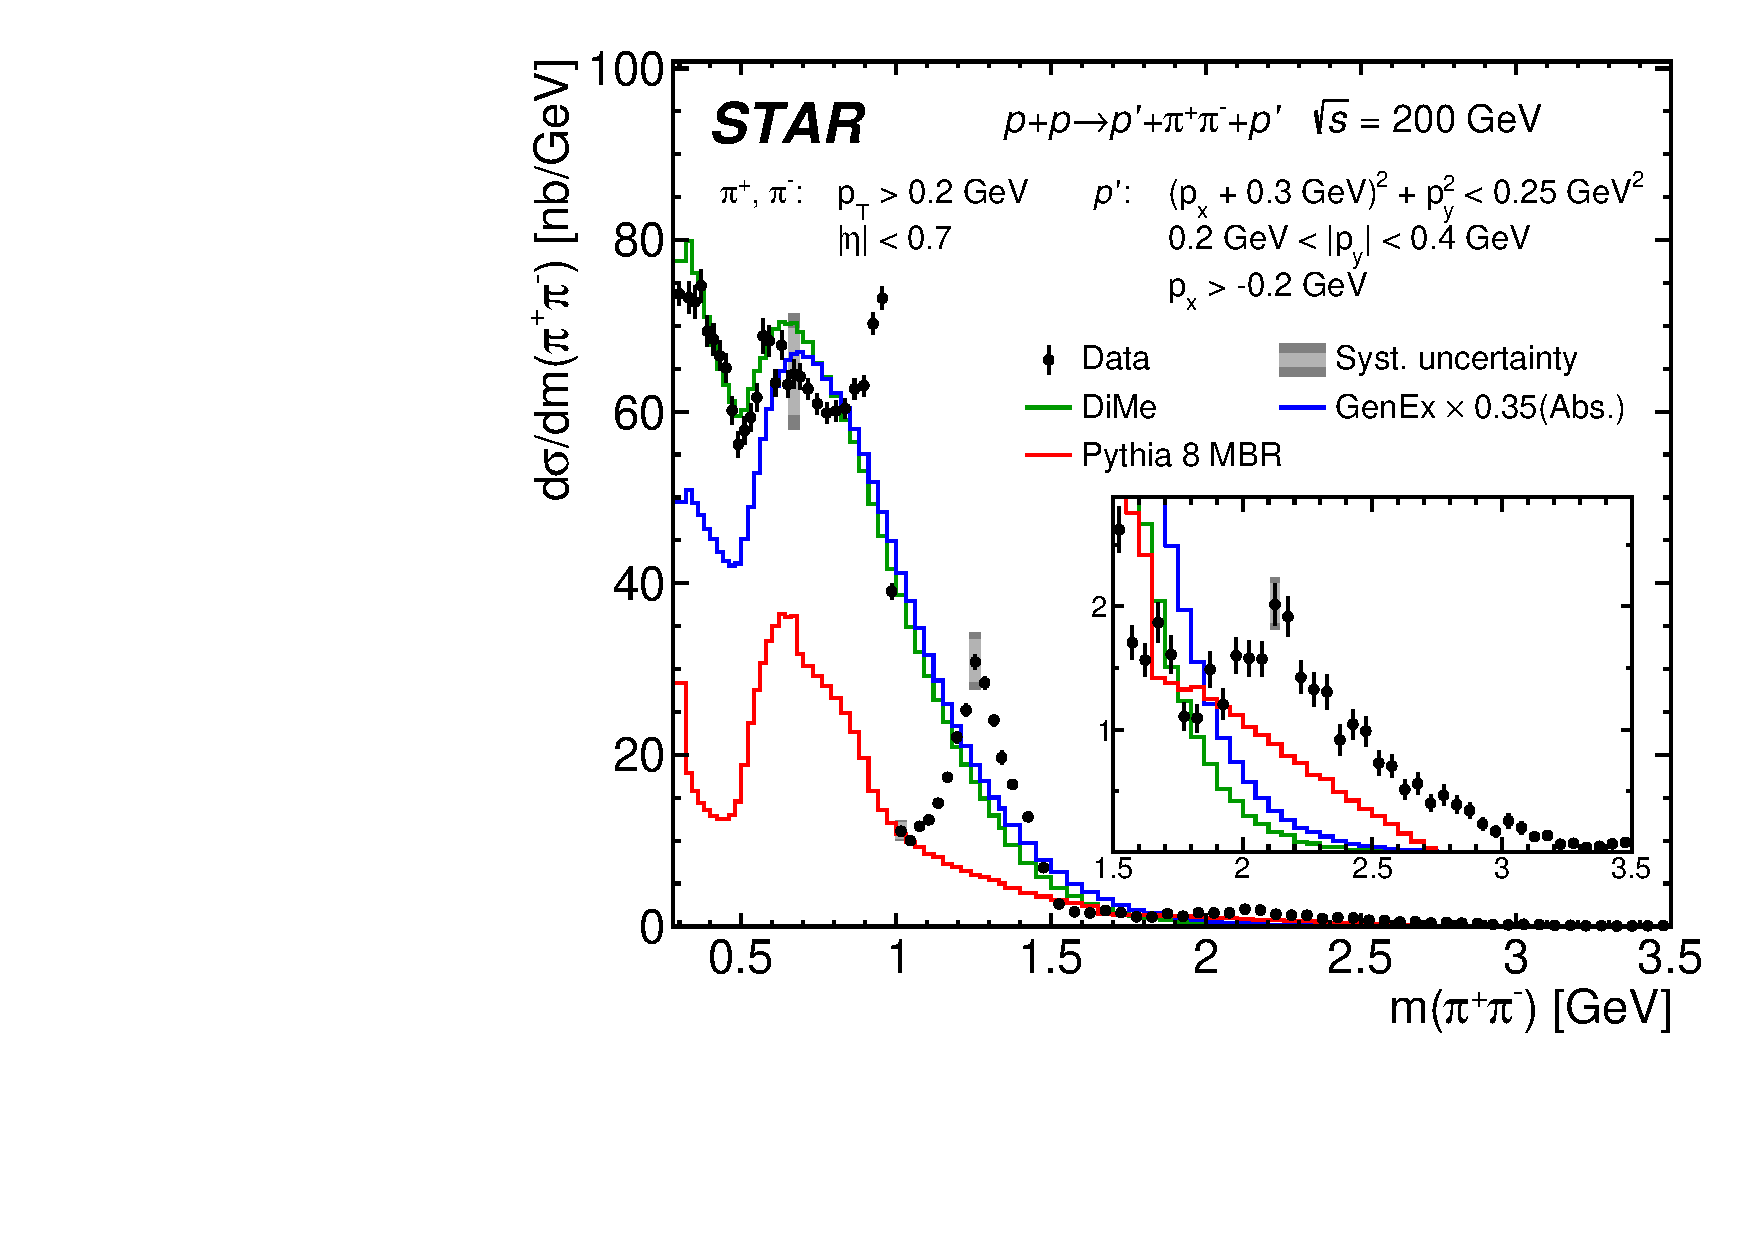
\includegraphics[width=.7\textwidth,page=1]{graphics/physicsResults/FinalResult_InvMass_pion.pdf}
%
\caption{Differential cross sections for CEP of charged particle pairs $\pi^+\pi^-$ as a function of the invariant mass of the pair in the fiducial region explained on the plots. Data are shown as solid points with error bars representing the statistical uncertainties. The typical systematic uncertainties are shown as gray boxes for only few data points as they are almost fully correlated between neighboring bins. Predictions from MC models GenEx, DiMe and MBR are shown as histograms. In the lower panels in the bottom plots the ratios of the MC predictions scaled to data and the data are shown.}
\label{results_01}
\end{figure}
%
\begin{figure}[h]
\centering
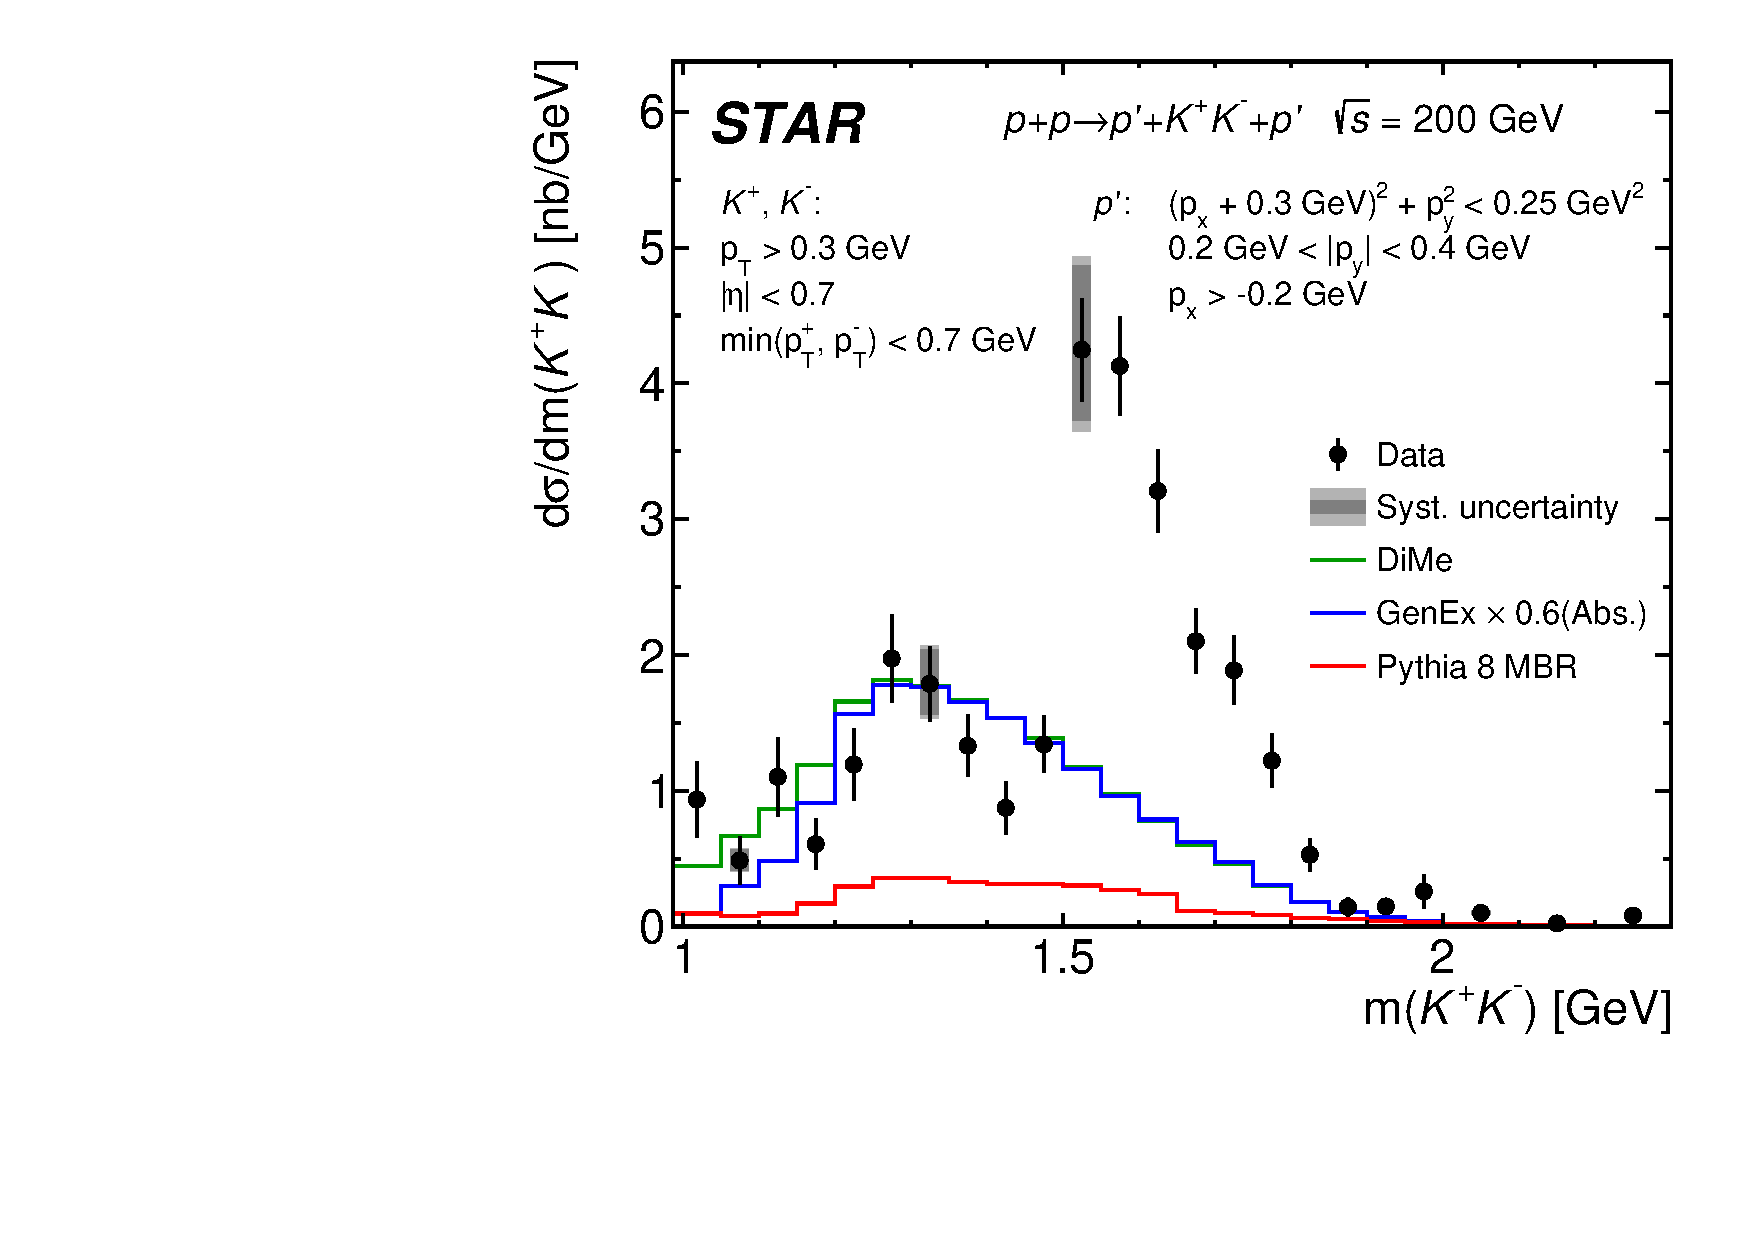
\includegraphics[width=.48\textwidth,page=1]{graphics/physicsResults/FinalResult_InvMass_kaon.pdf}
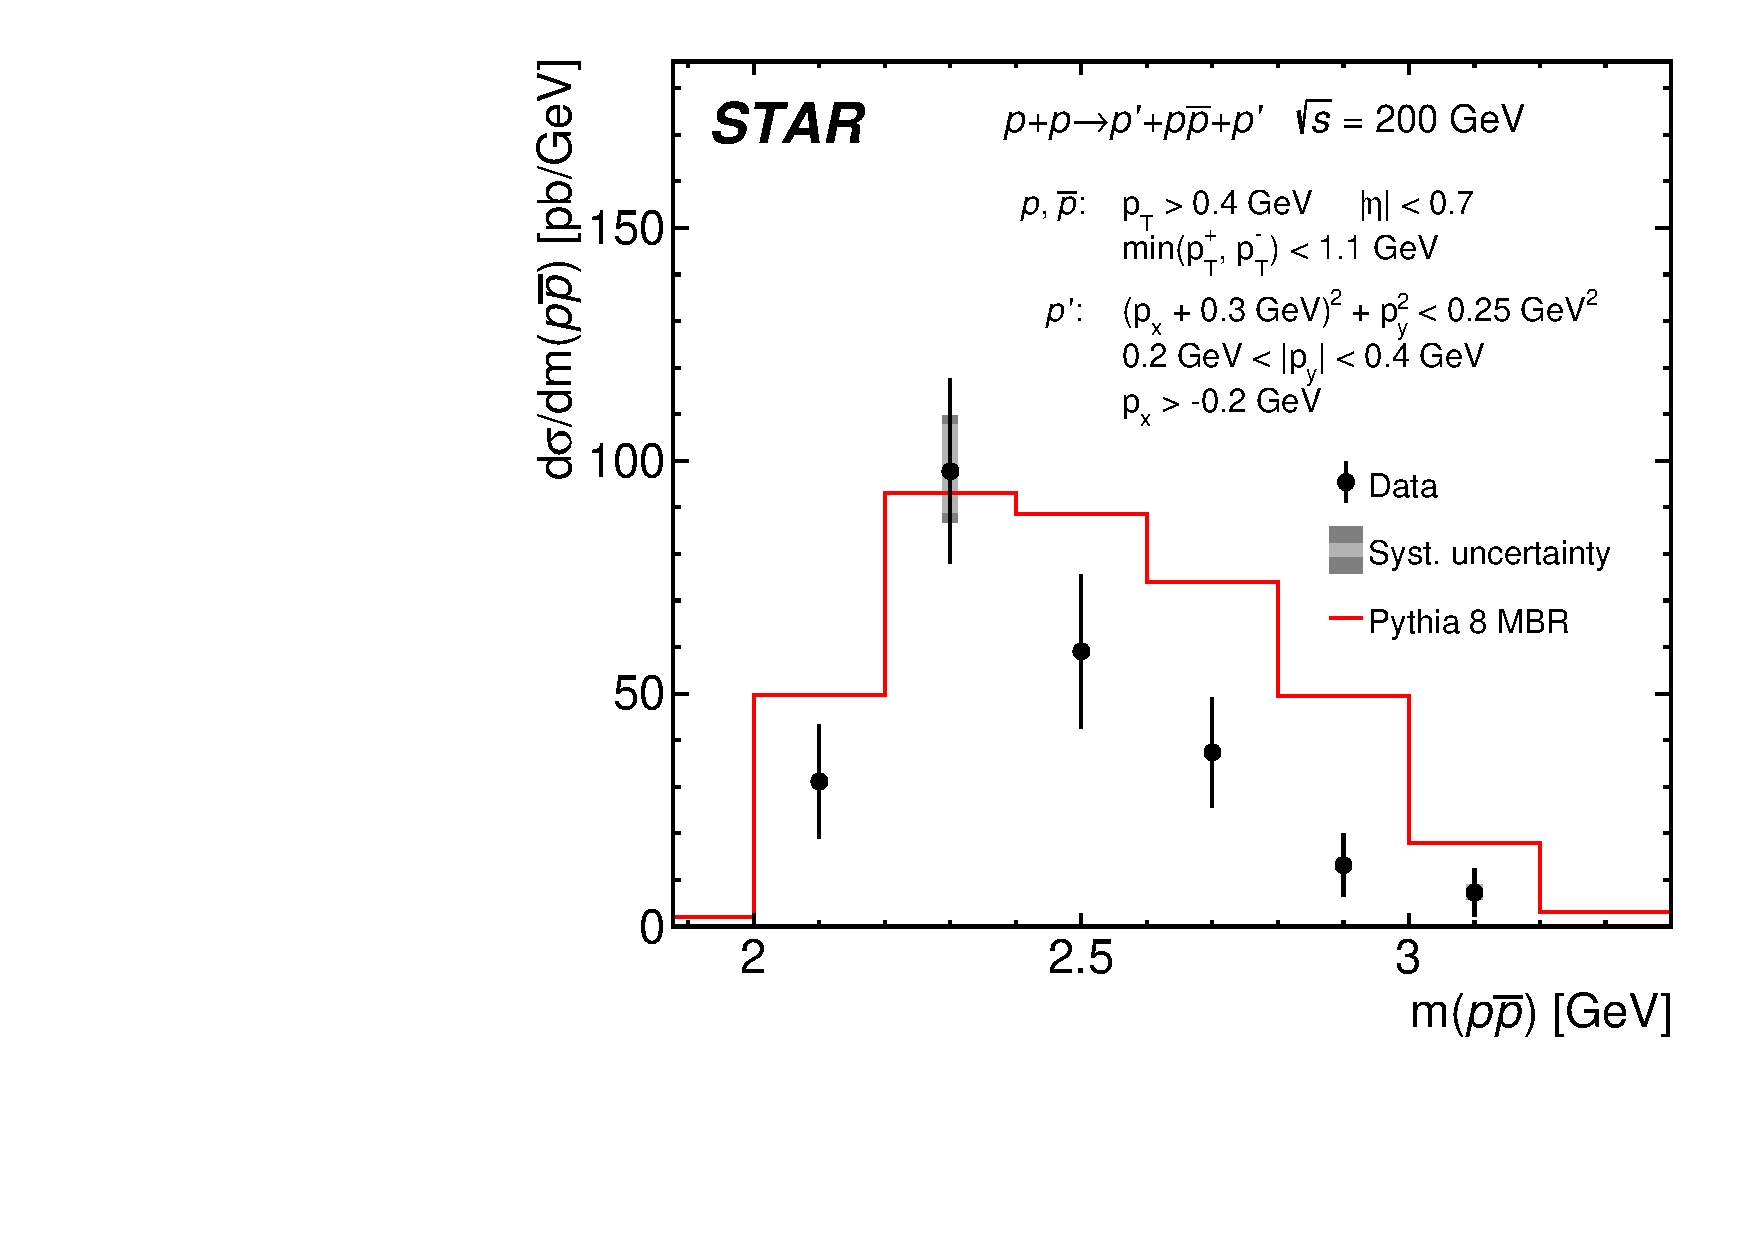
\includegraphics[width=.48\textwidth,page=1]{graphics/physicsResults/FinalResult_InvMass_proton.pdf}
%
\caption{Differential cross sections for CEP of charged particle pairs $K^+K^-$ (left) and $p\bar{p}$ (right) as a function of the invariant mass of the pair in the fiducial region explained on the plots. Data are shown as solid points with error bars representing the statistical uncertainties. The typical systematic uncertainties are shown as gray boxes for only few data points as they are almost fully correlated between neighboring bins. Predictions from MC models GenEx, DiMe and MBR are shown as histograms. In the lower panels in the bottom plots the ratios of the MC predictions scaled to data and the data are shown.}
\label{results_02}
\end{figure}
% 
\begin{figure}[h]
\centering
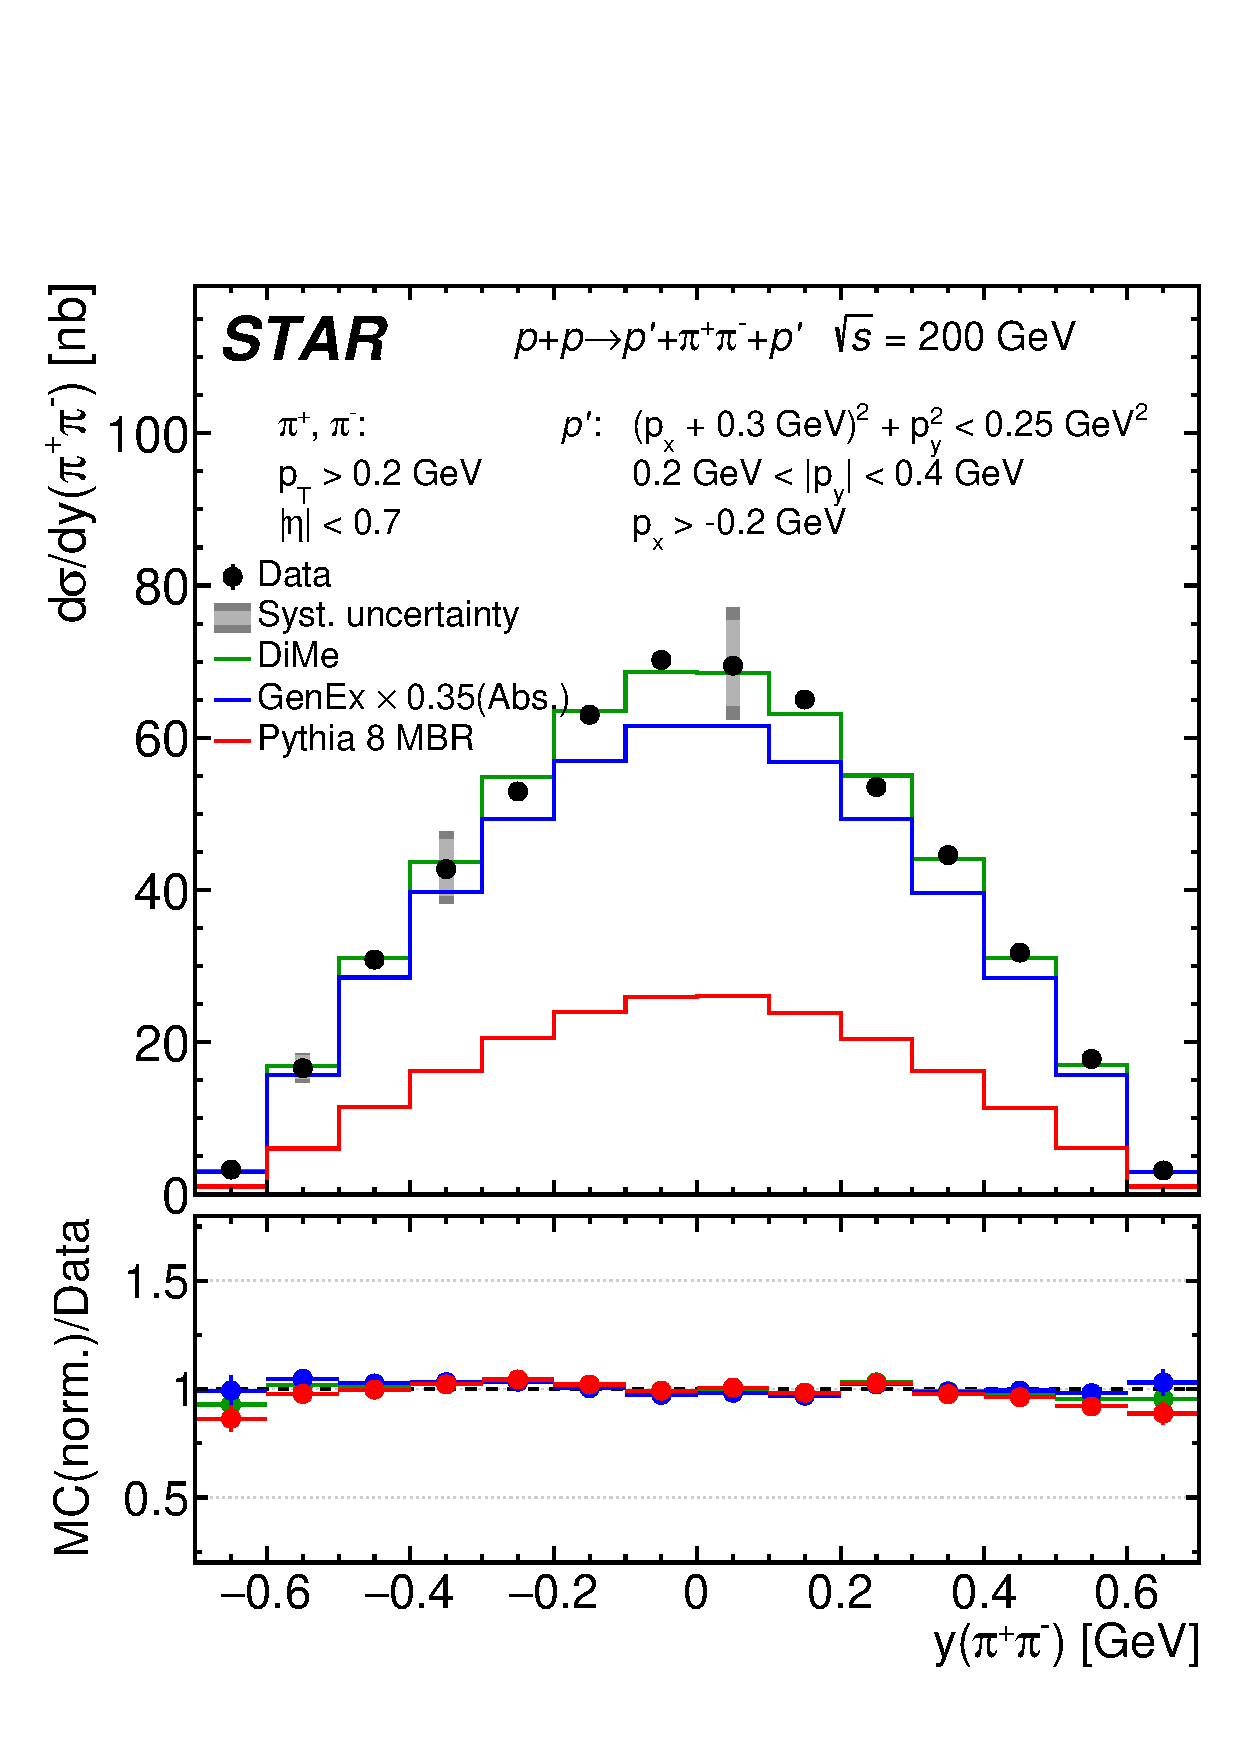
\includegraphics[width=.31\textwidth,page=1]{graphics/physicsResults/Ratio_FinalResult_Rapidity_pion.pdf}
\hfill
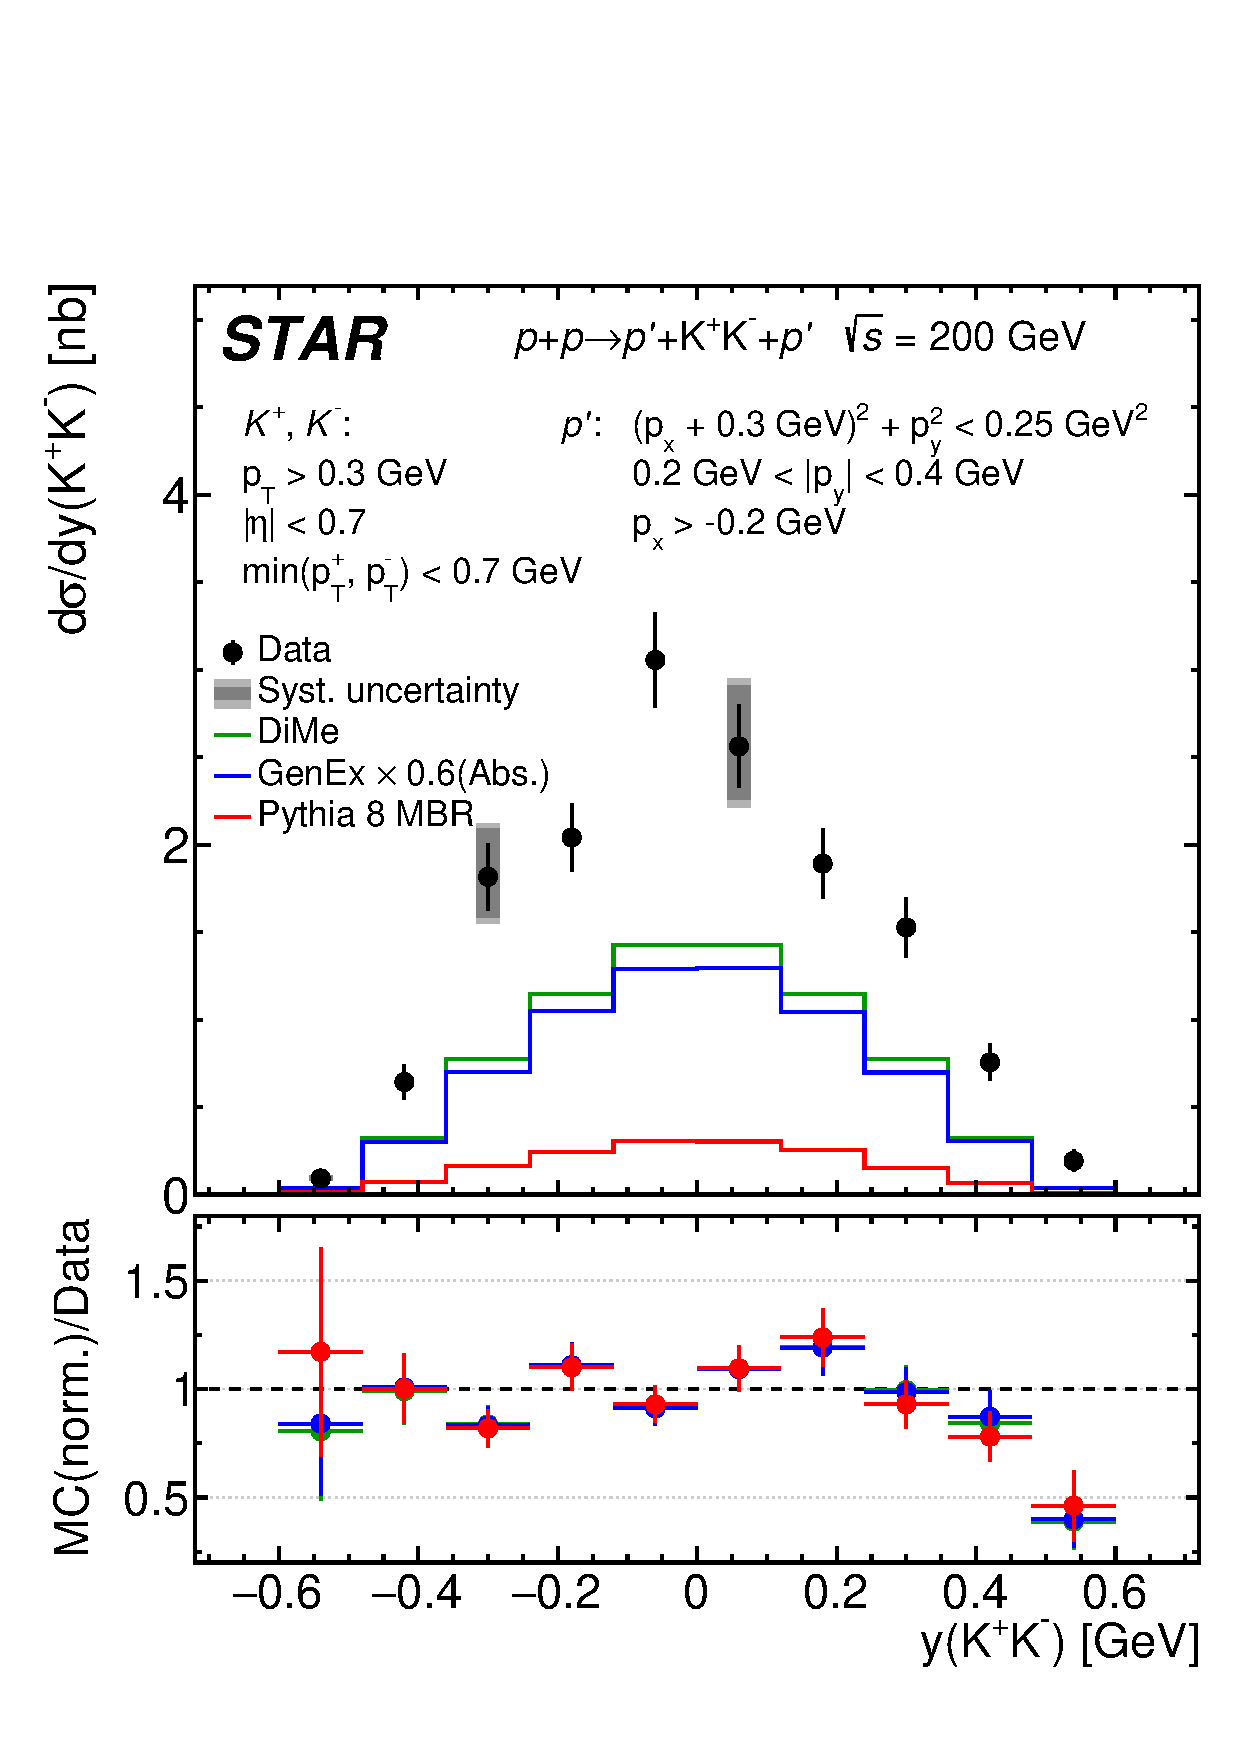
\includegraphics[width=.31\textwidth,page=1]{graphics/physicsResults/Ratio_FinalResult_Rapidity_kaon.pdf}
\hfill
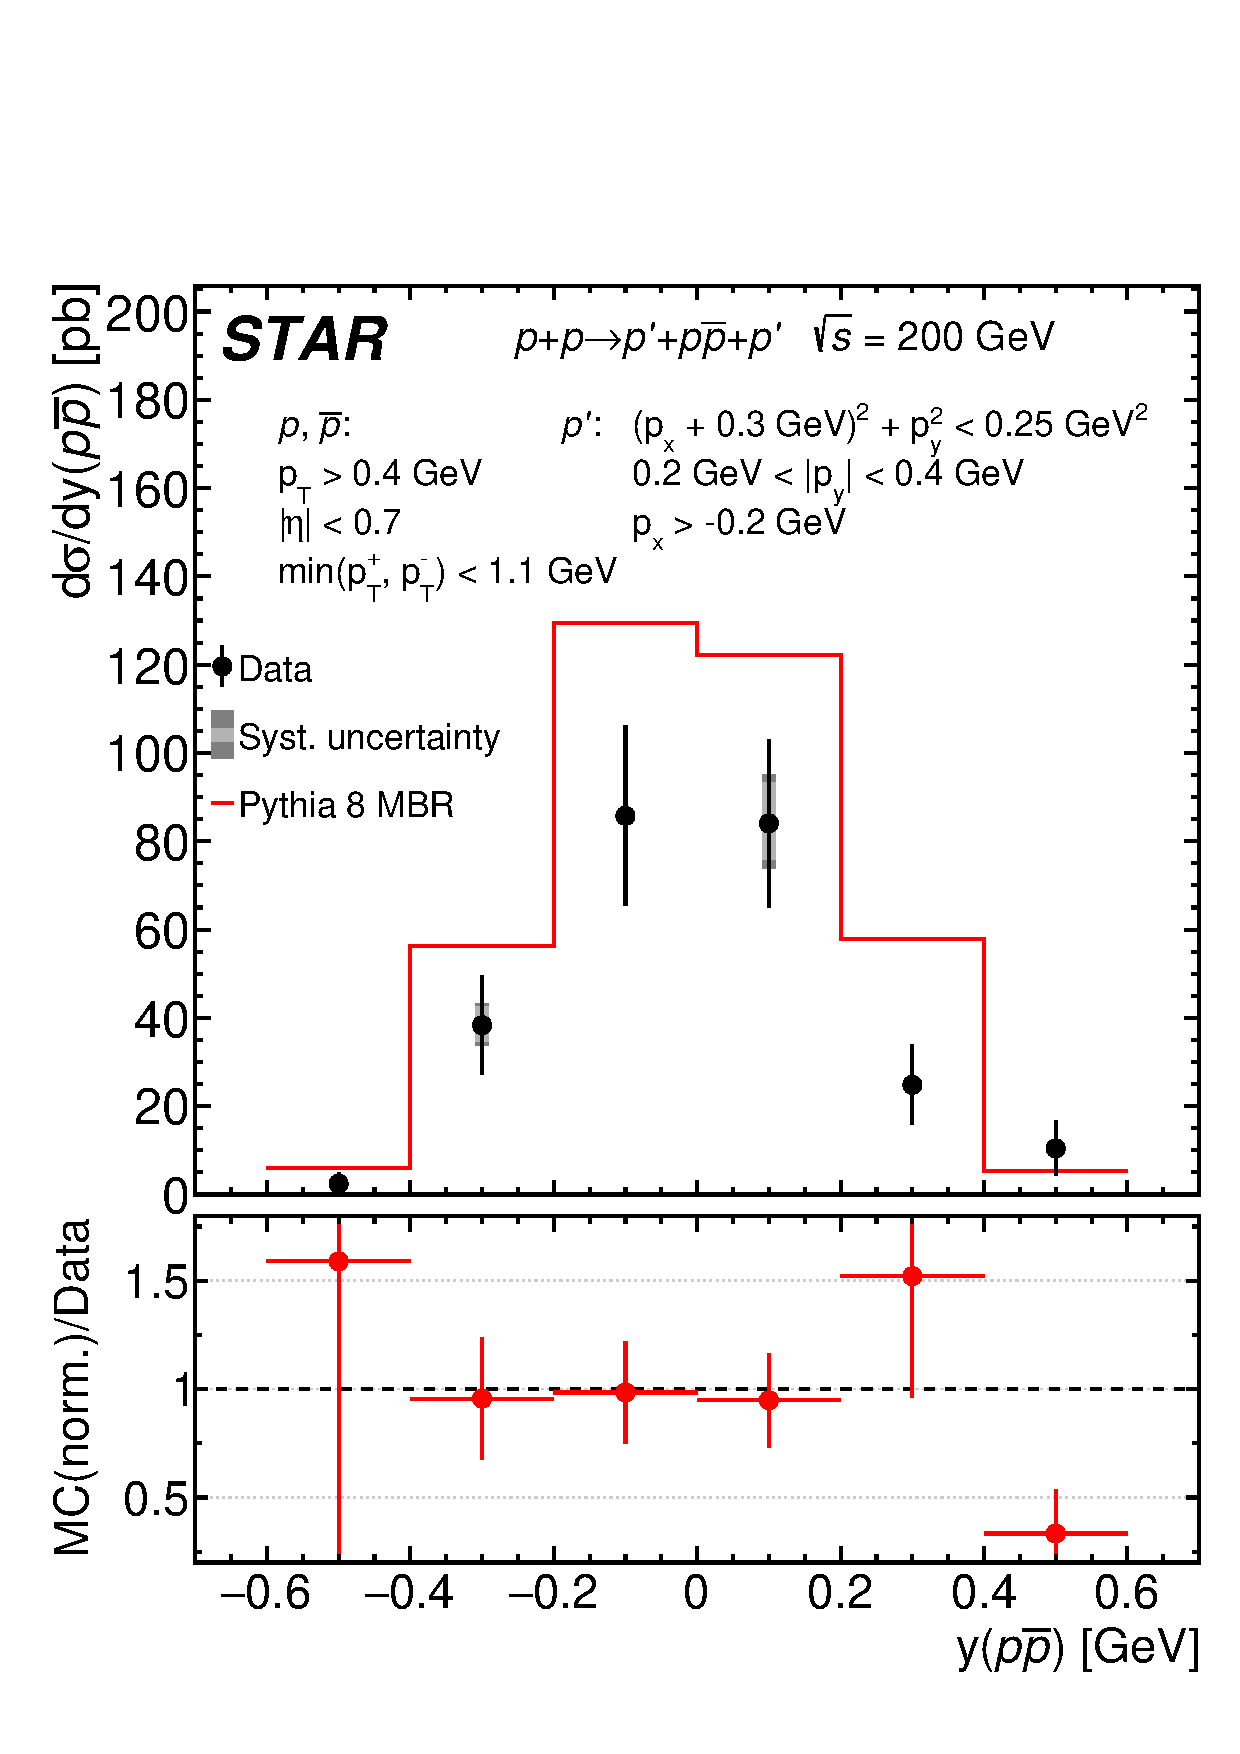
\includegraphics[width=.31\textwidth,page=1]{graphics/physicsResults/Ratio_FinalResult_Rapidity_proton.pdf}
%
\caption{Differential cross sections for CEP of charged particle pairs $\pi^+\pi^-$ (let), $K^+K^-$ (middle) and $p\bar{p}$ (right) as a function of the pair rapidity measured in the fiducial region explained on the plots. Data are shown as solid points with error bars representing the statistical uncertainties. The typical systematic uncertainties are shown as gray boxes for only few data points as they are almost fully correlated between neighboring bins. Predictions from MC models GenEx, DiMe and MBR are shown as histograms. In the lower panels in the bottom plots the ratios of the MC predictions scaled to data and the data are shown.}
\label{results_1}
\end{figure}
%
% \indent
% Figure~\ref{results_2}(right column) shows the differential cross sections for CEP of different particle species pairs as a function of the sum of the squares of the four-momenta transfers at the proton vertices.
% %
% The shapes of measured cross sections are strongly affected by the fiducial cuts applied to the forward scattered protons.
% %
% The shapes of the differential cross sections for both $\pi^+\pi^-$ snd $K^+K^-$ pairs production are better described by the DiMe model than by GenEx and MBR models.
% In case of the cross section for $p\bar{p}$ pairs production the MBR model implemented in PYTHIA8 describes normalization of the data fairly well but predicts a steeper slope.\\
% %
% \indent
% Figure~\ref{results_3} shows the differential cross sections for CEP of different particle species pairs as a function of the pair invariant mass separately in two $\Delta\phi$ regions: $\Delta\phi<90$ degree (left column) and $\Delta\phi>90$ degree (right column).
% %
% Sharp drops of the measured cross sections at $m(\pi^+\pi^-) < 0.6$~GeV and at $m(K^+K^-) < 1.3$~GeV for the $\Delta\phi>$ 90 degree range are due to the fiducial cuts applied to the forward scattered protons. 
% %
% In case of the cross section for CEP of $\pi^+\pi^-$ pairs in $\Delta\phi<90$ degree range the peak around $f_2(1270)$ resonance in data is significantly suppressed while the peak at $f_0(980)$ is enhanced as well as possible resonances in the mass range $1.3-1.5$ MeV compared to the $\Delta\phi>90$ degrees range. 
%
\begin{figure}[h]
\centering
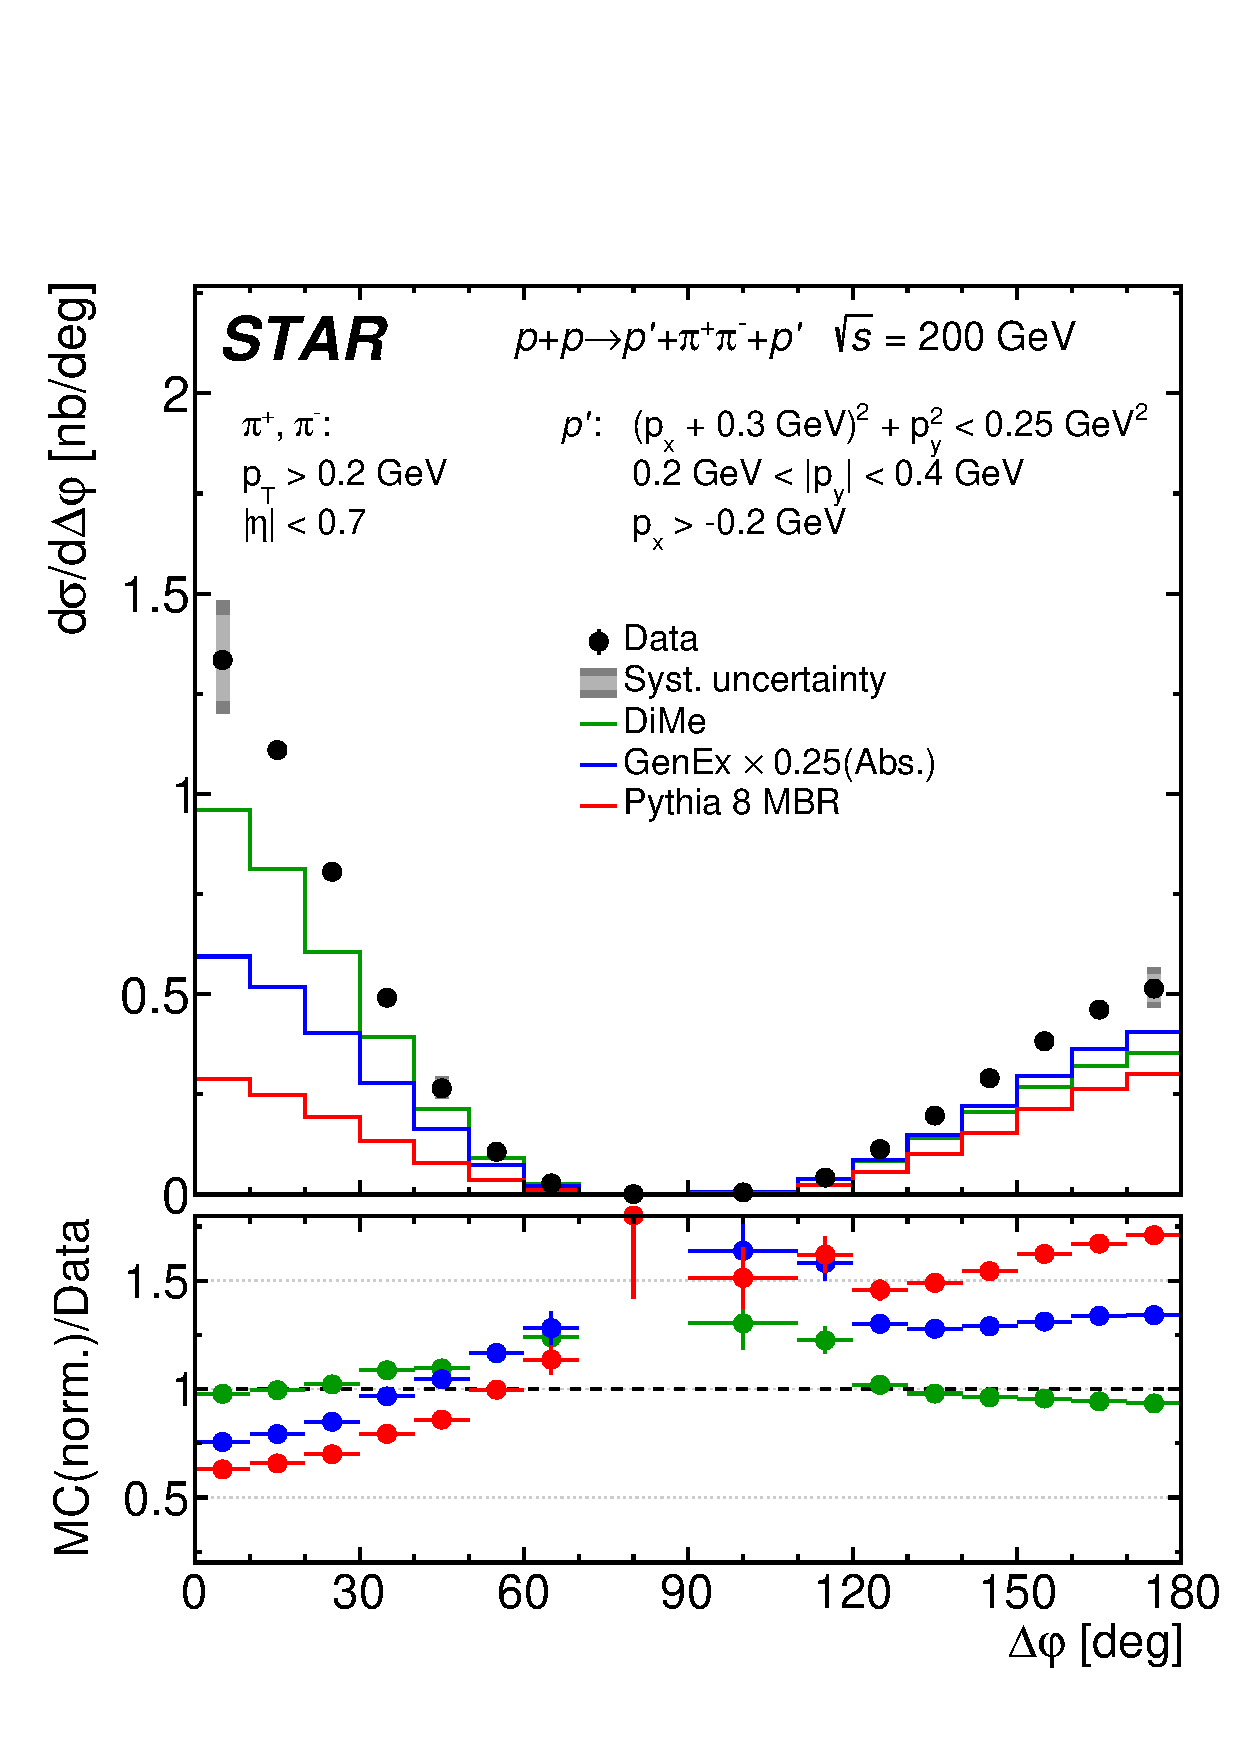
\includegraphics[width=.31\textwidth,page=1]{graphics/physicsResults/Ratio_FinalResult_DeltaPhi_pion.pdf}
\hfill
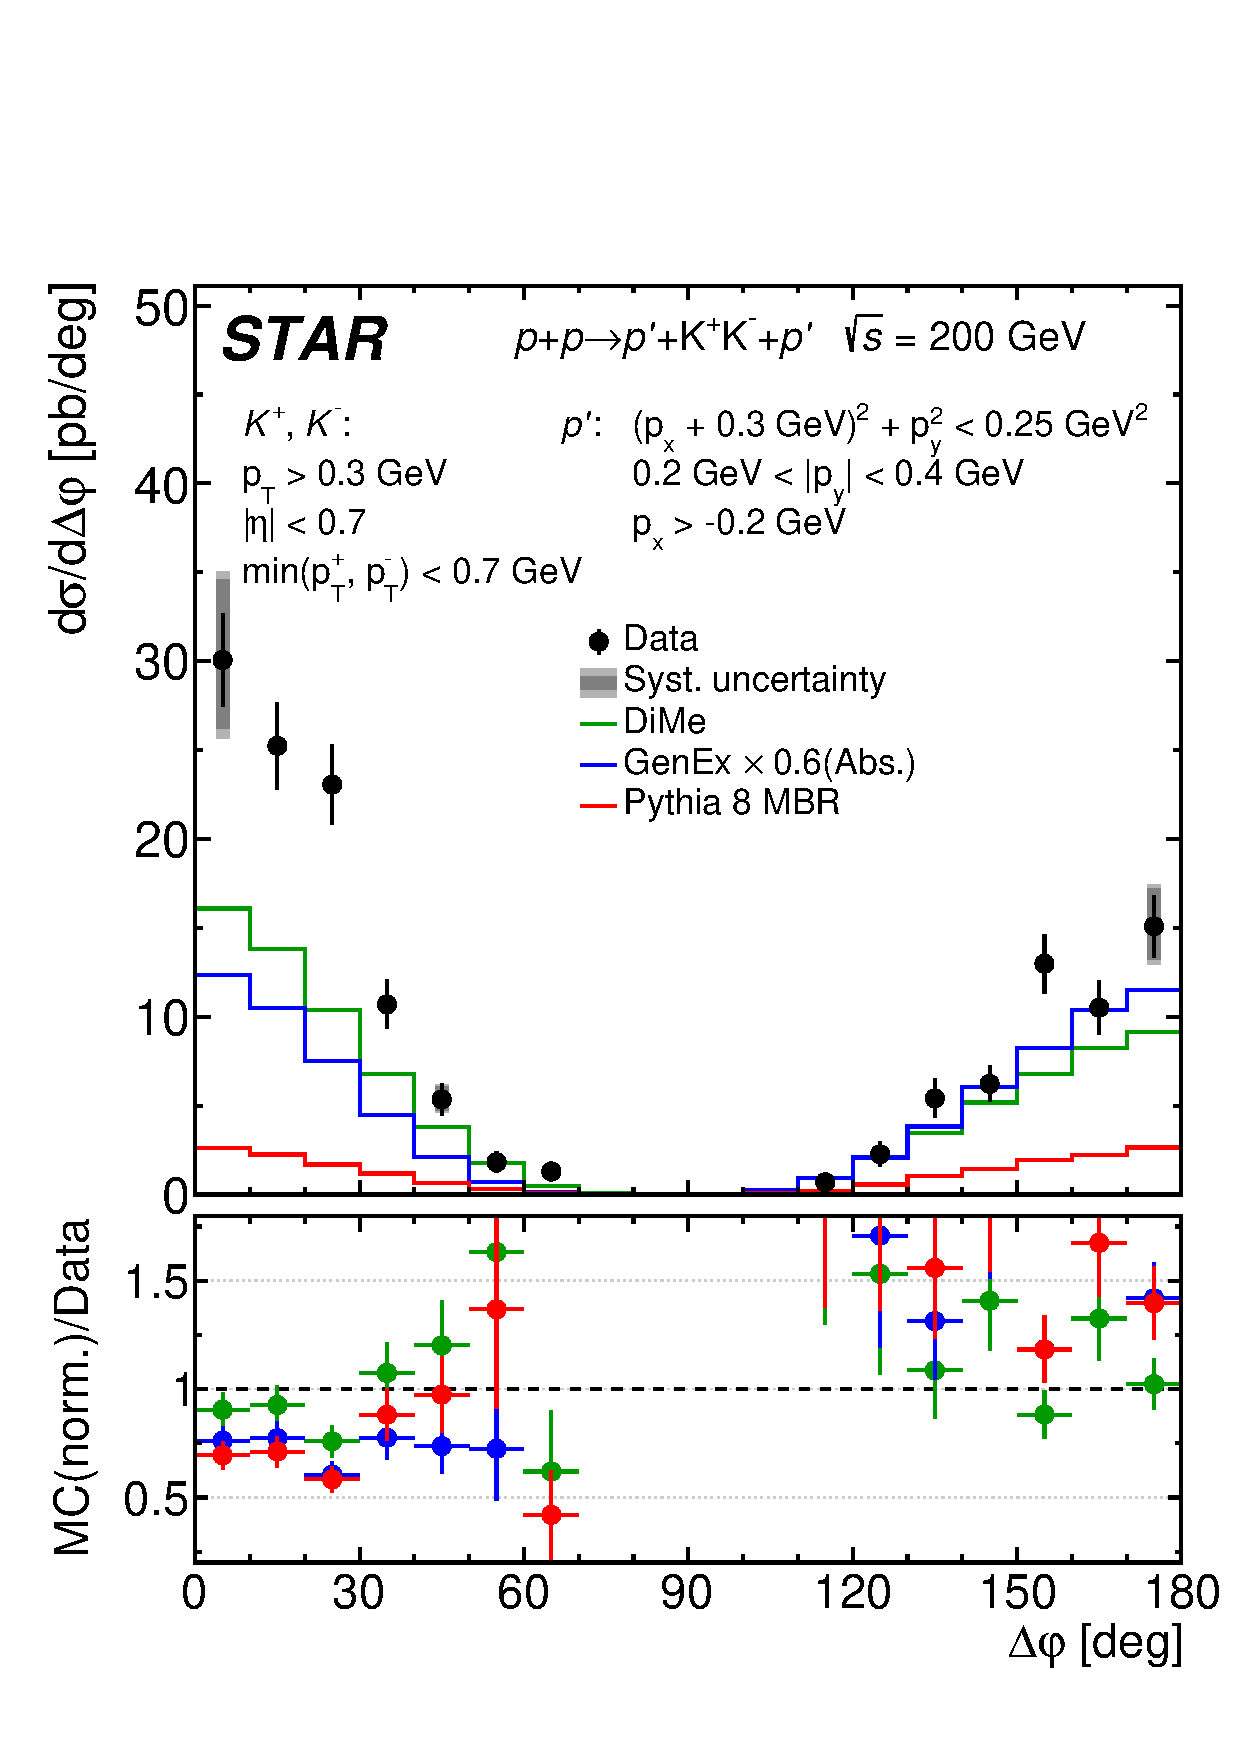
\includegraphics[width=.31\textwidth,page=1]{graphics/physicsResults/Ratio_FinalResult_DeltaPhi_kaon.pdf}
\hfill
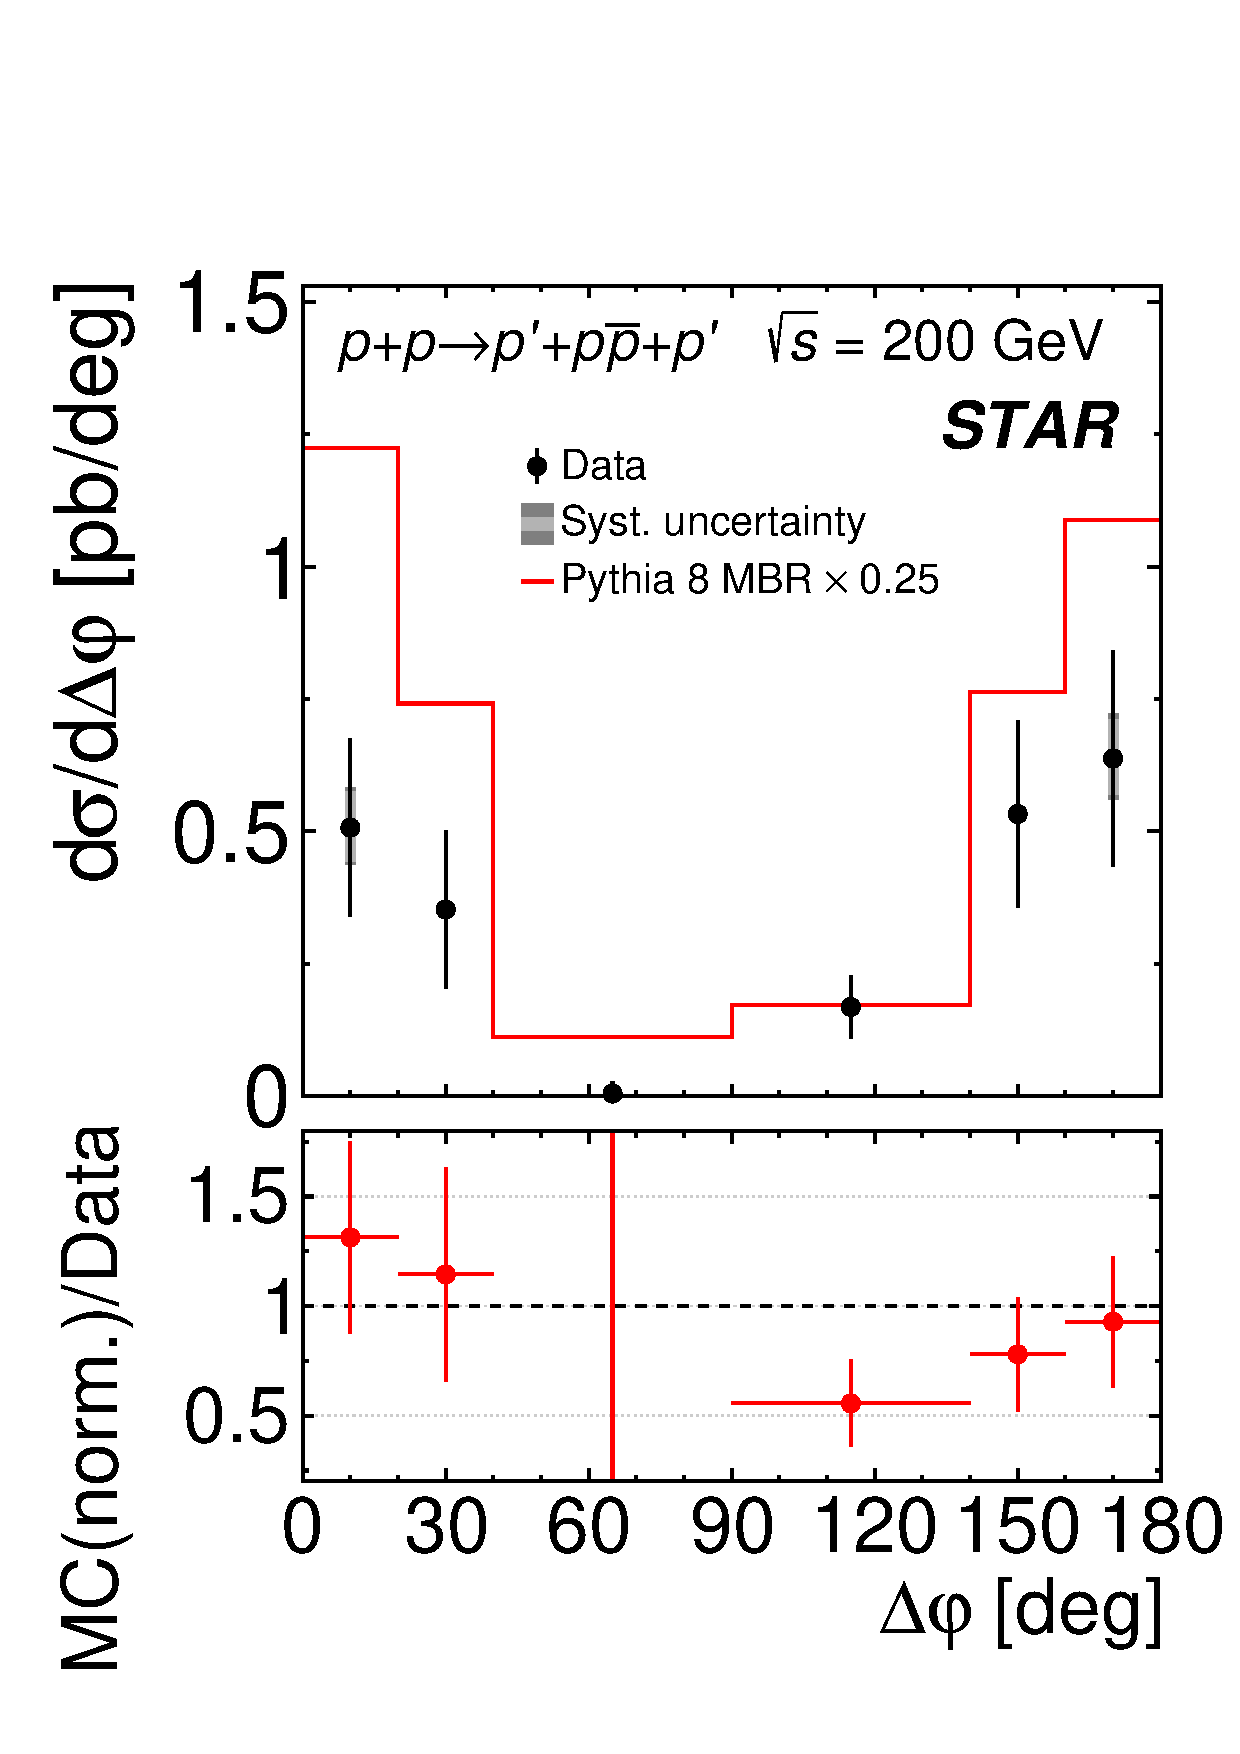
\includegraphics[width=.31\textwidth,page=1]{graphics/physicsResults/Ratio_FinalResult_DeltaPhi_proton.pdf}
\newline
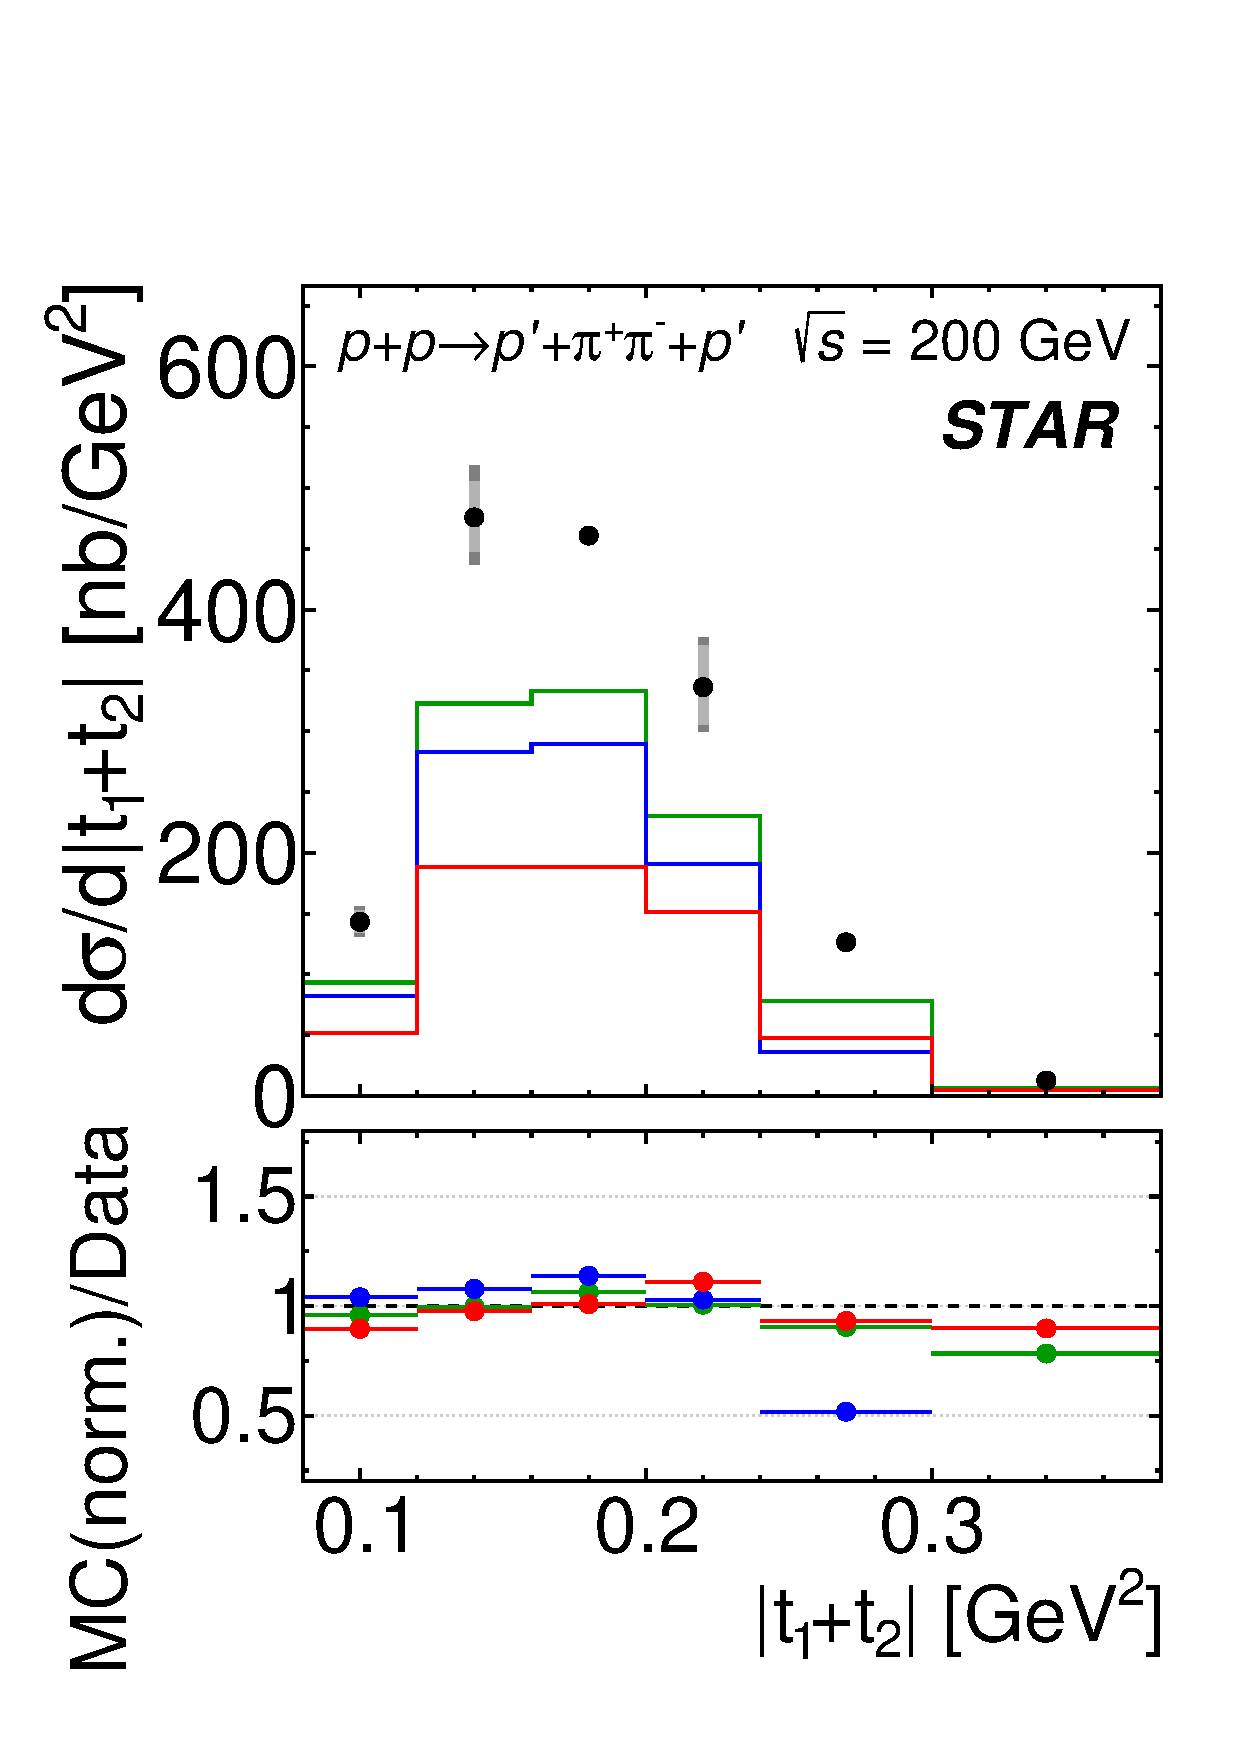
\includegraphics[width=.31\textwidth,page=1]{graphics/physicsResults/Ratio_FinalResult_MandelstamTSum_pion.pdf}
\hfill
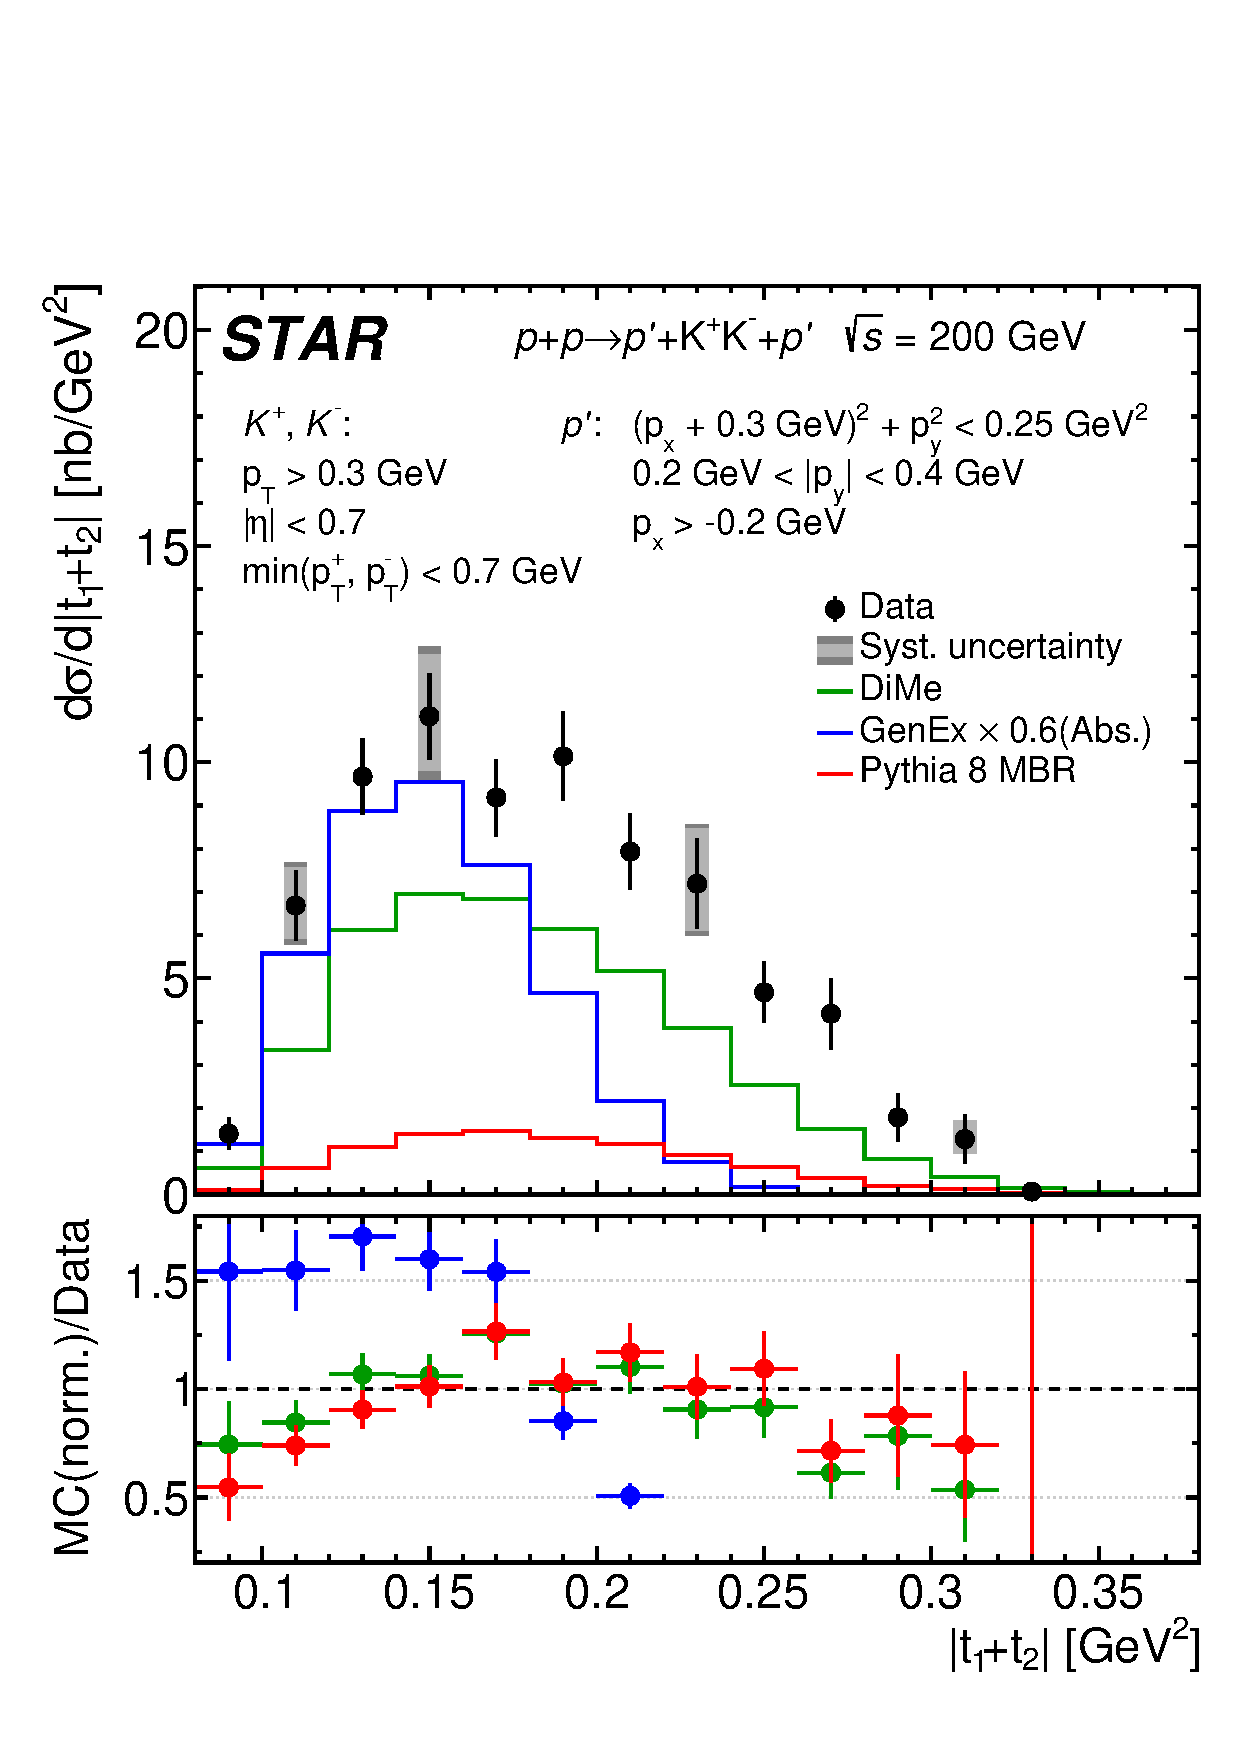
\includegraphics[width=.31\textwidth,page=1]{graphics/physicsResults/Ratio_FinalResult_MandelstamTSum_kaon.pdf}
\hfill
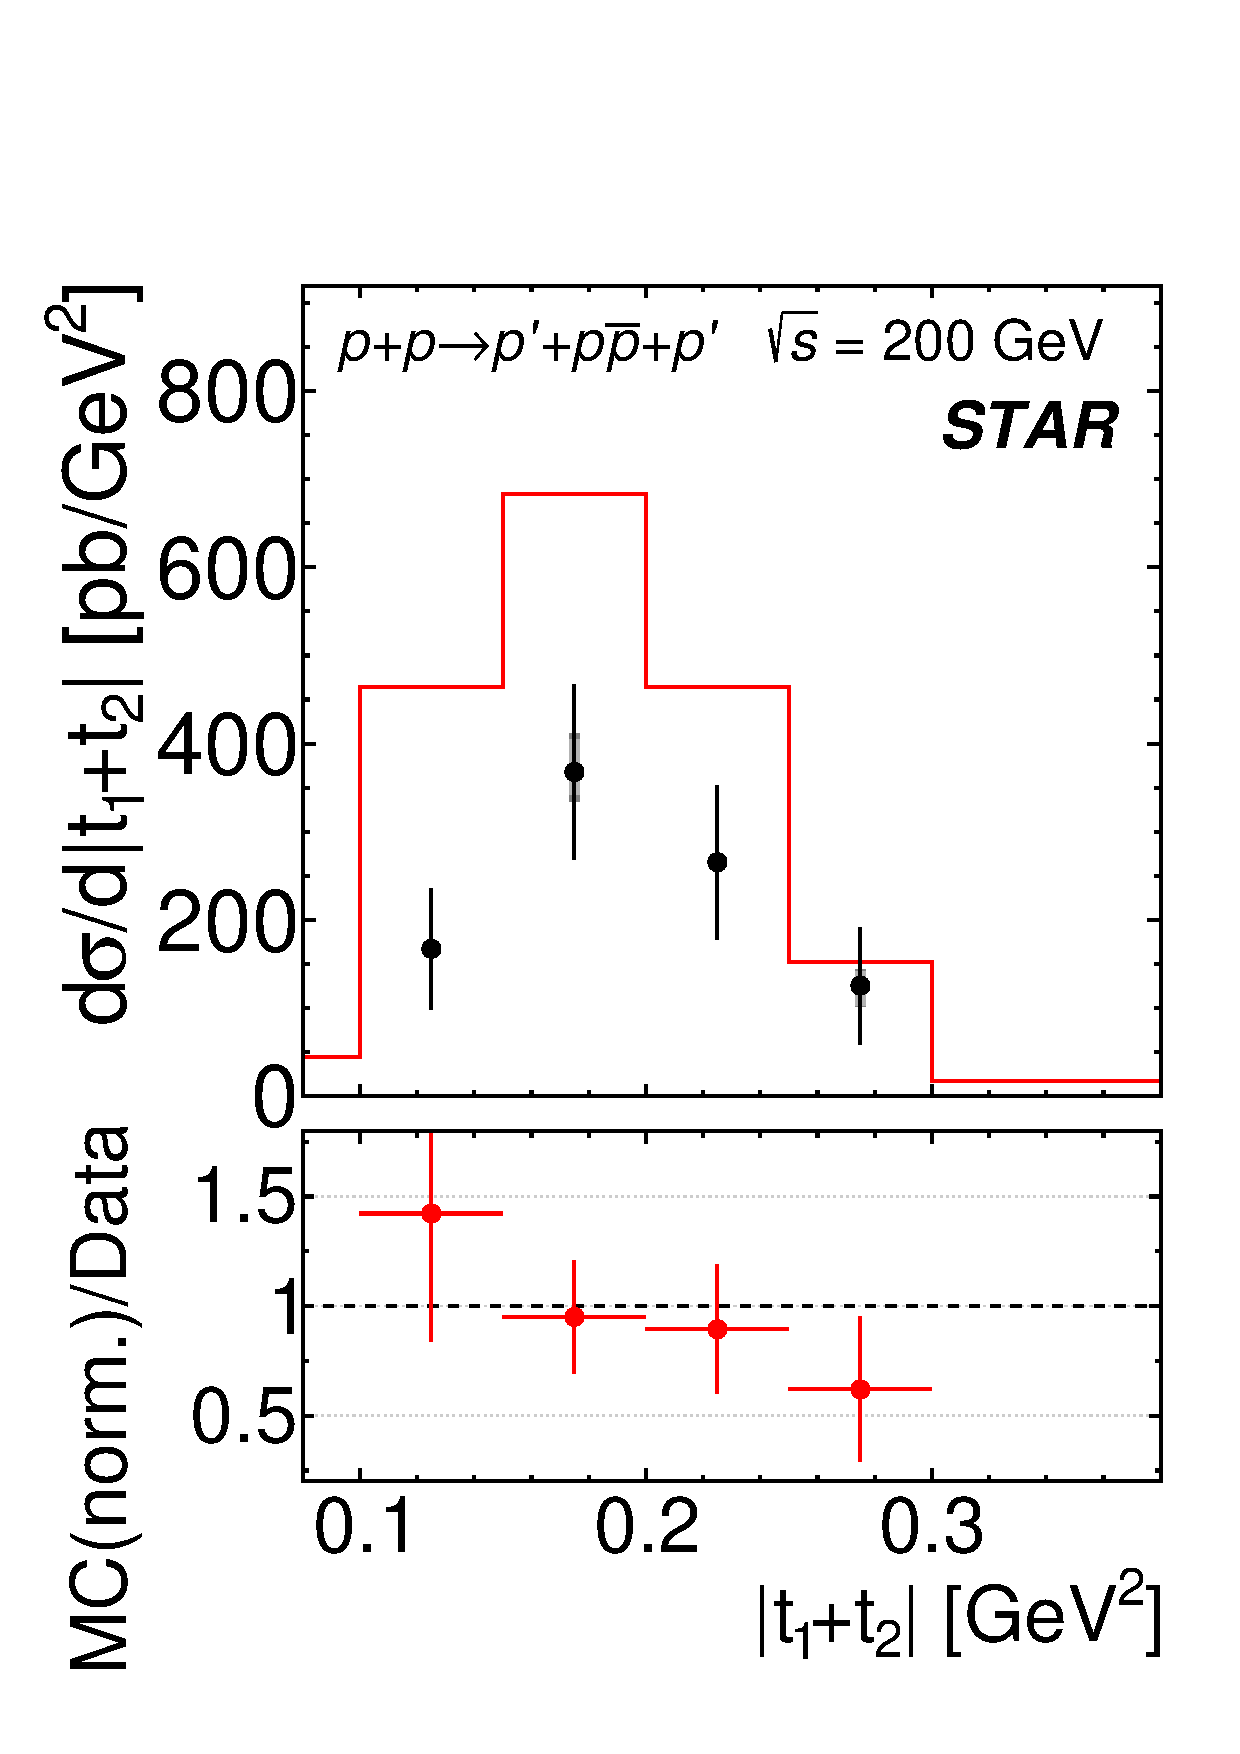
\includegraphics[width=.31\textwidth,page=1]{graphics/physicsResults/Ratio_FinalResult_MandelstamTSum_proton.pdf}
%
\caption{Differential cross sections for CEP of charged particle pairs $\pi^+\pi^-$ (left column), $K^+K^-$ (middle column) and $p\bar{p}$ (right column) as a function of the difference of azimuthal angles of the forward scattered protons (top) and of the sum of the squares of the four-momenta losses in the proton vertices (bottom) measured in the fiducial region explained on the plots. Data are shown as solid points with error bars representing the statistical uncertainties. The typical systematic uncertainties are shown as gray boxes for only few data points as they are almost fully correlated between neighboring bins. Predictions from MC models GenEx, DiMe and MBR are shown as histograms. In the lower panels the ratios of the MC predictions scaled to data and the data are shown.}
\label{results_2}
\end{figure}
%
\begin{figure}[h]
\centering
\hspace*{5pt}
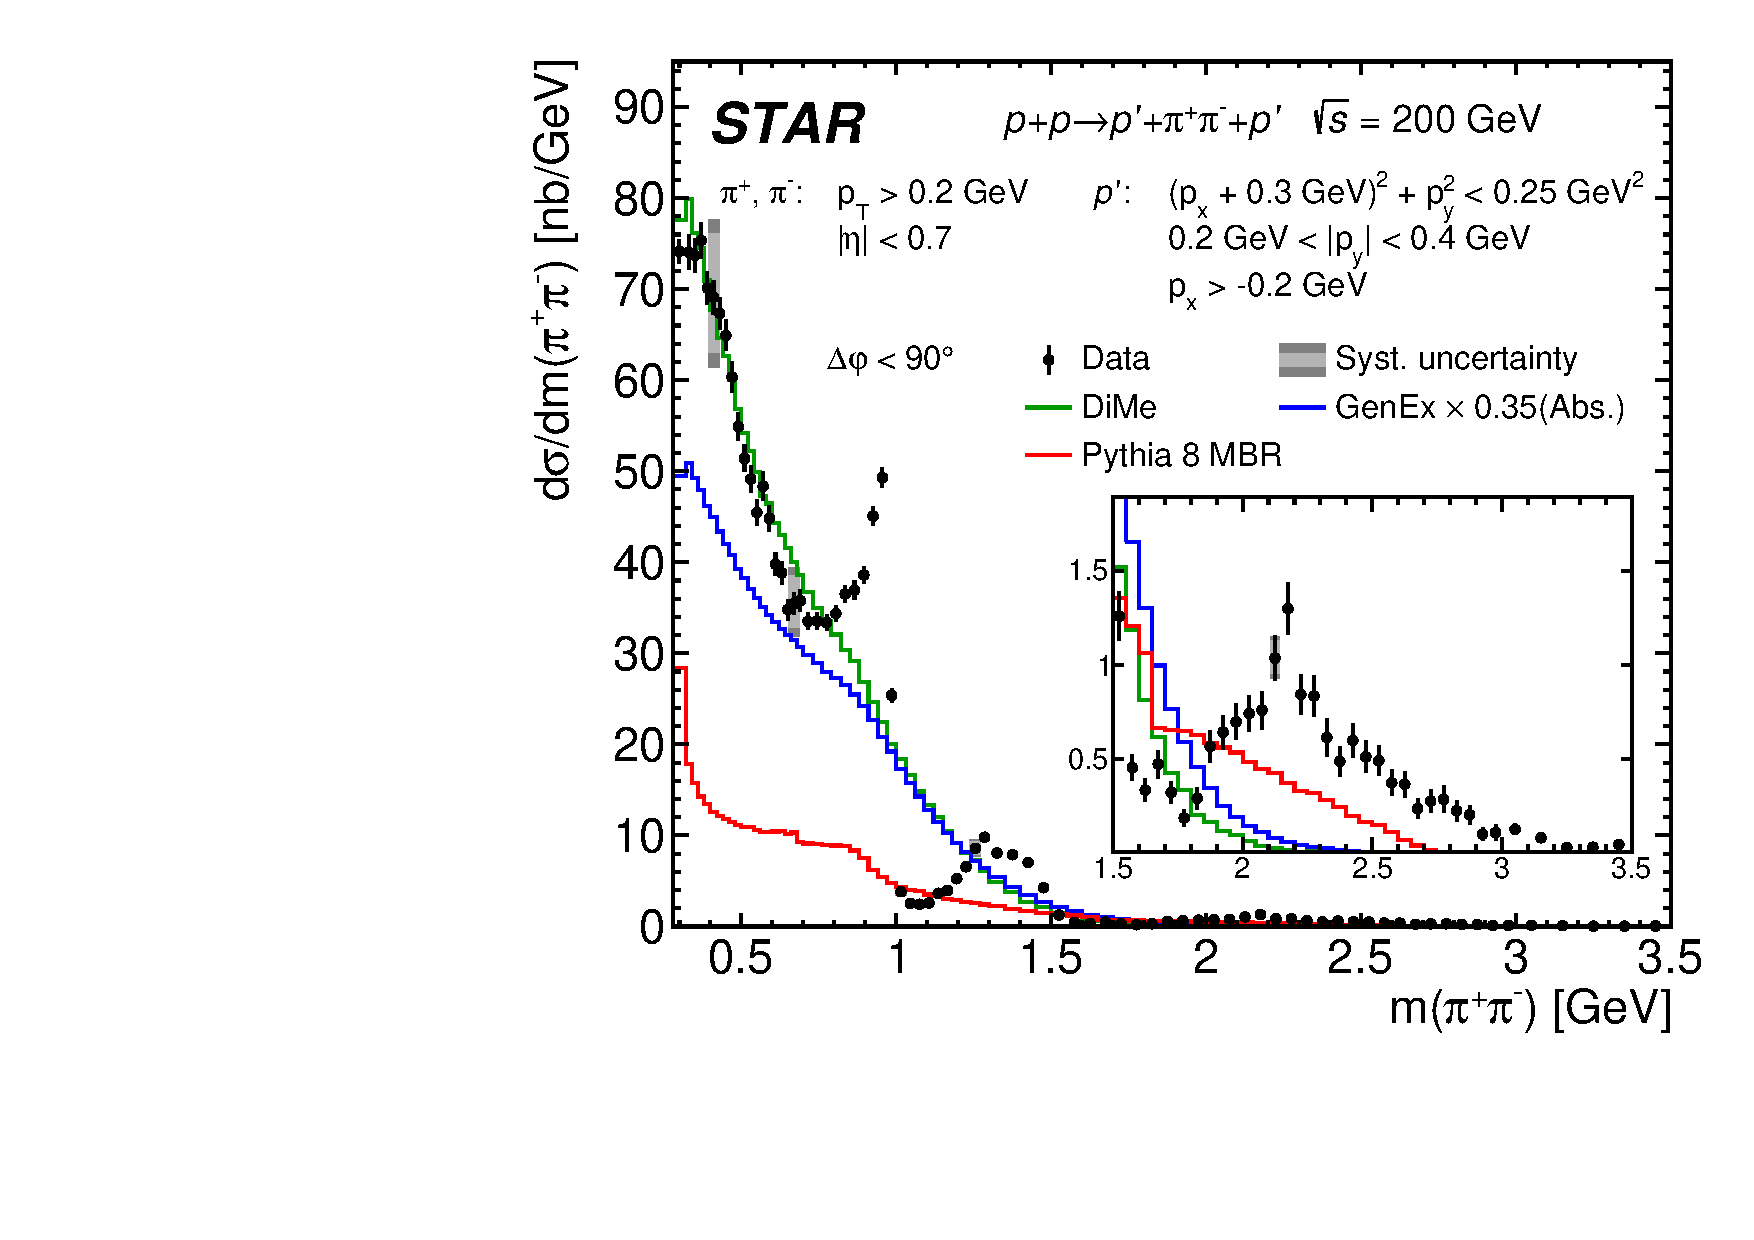
\includegraphics[width=.46\textwidth,page=1]{graphics/physicsResults/FinalResult_InvMass_DeltaPhiBin1_pion.pdf}
\hfill
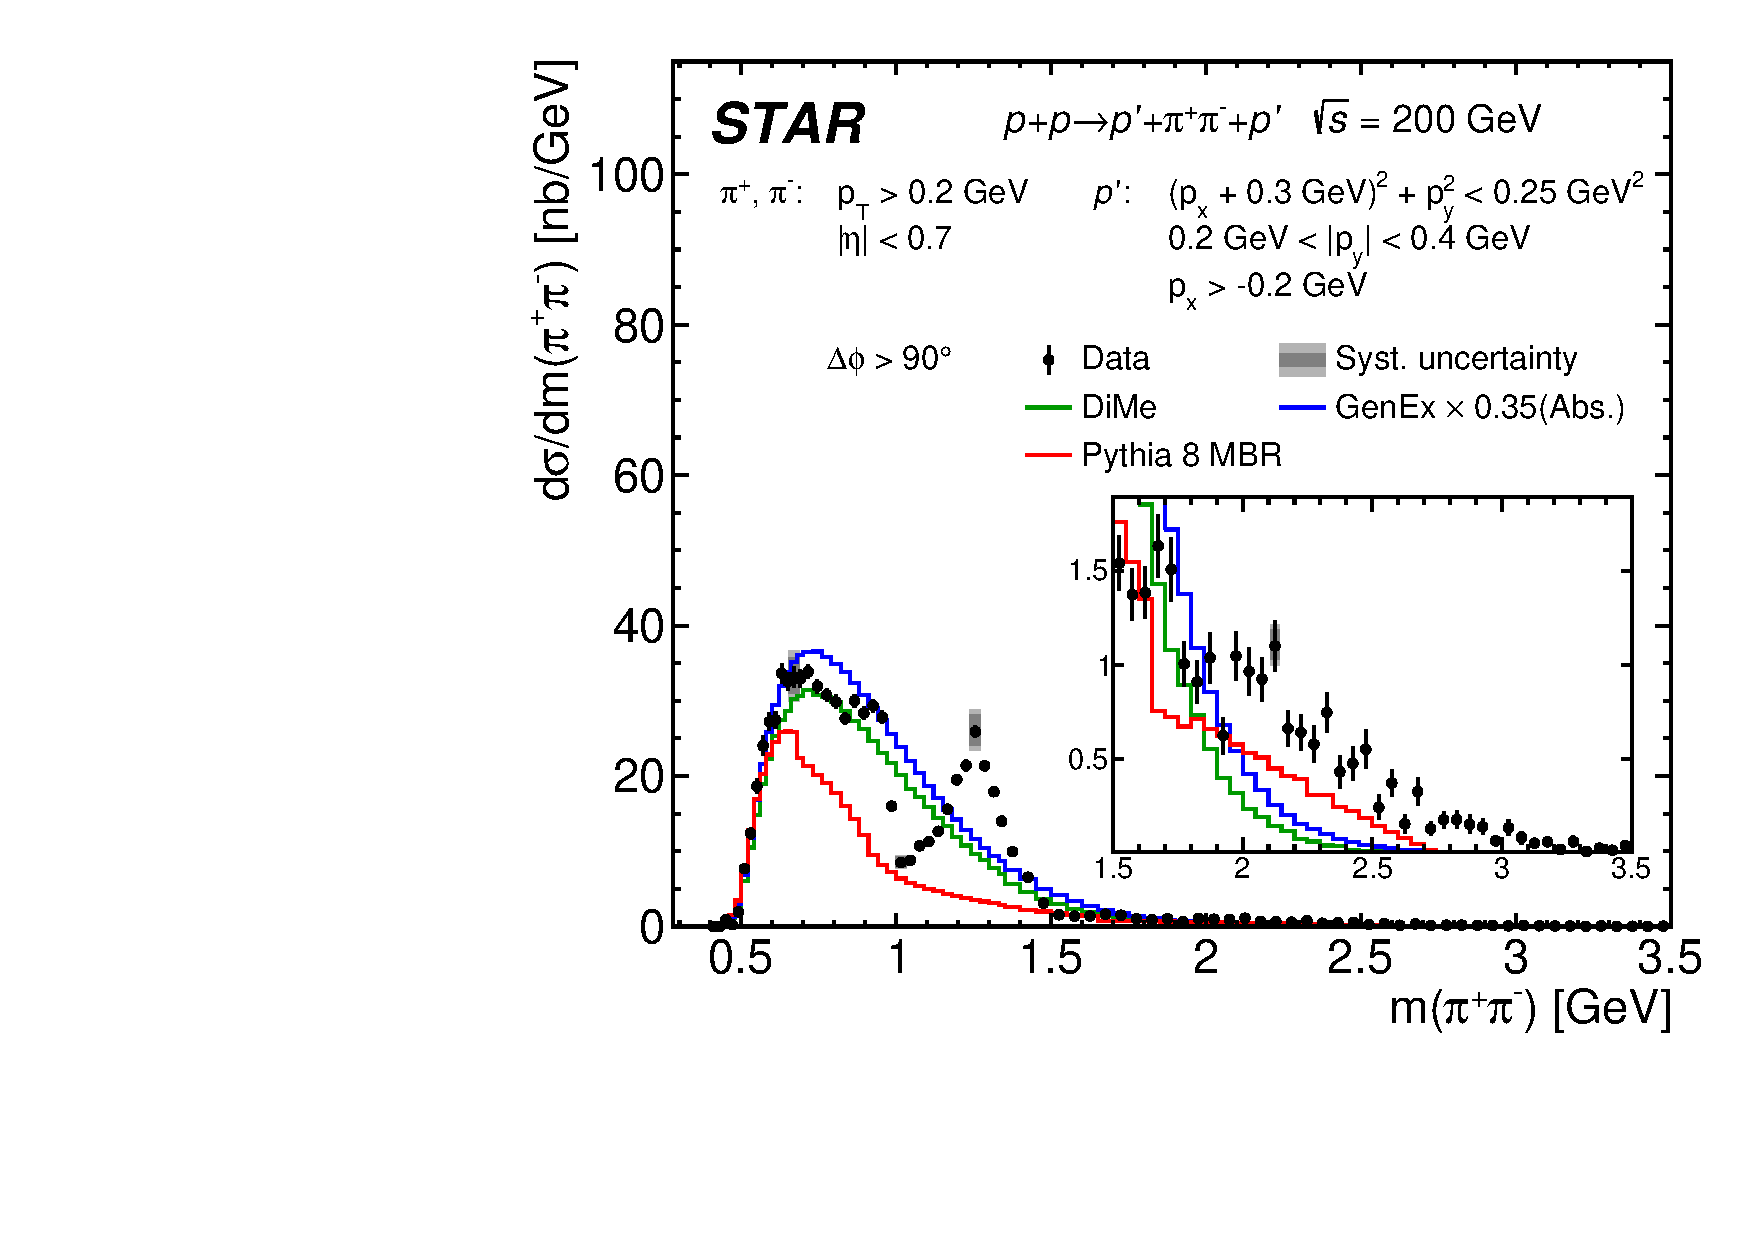
\includegraphics[width=.46\textwidth,page=1]{graphics/physicsResults/FinalResult_InvMass_DeltaPhiBin2_pion.pdf}
\hspace*{5pt}
\newline
\hspace*{5pt}
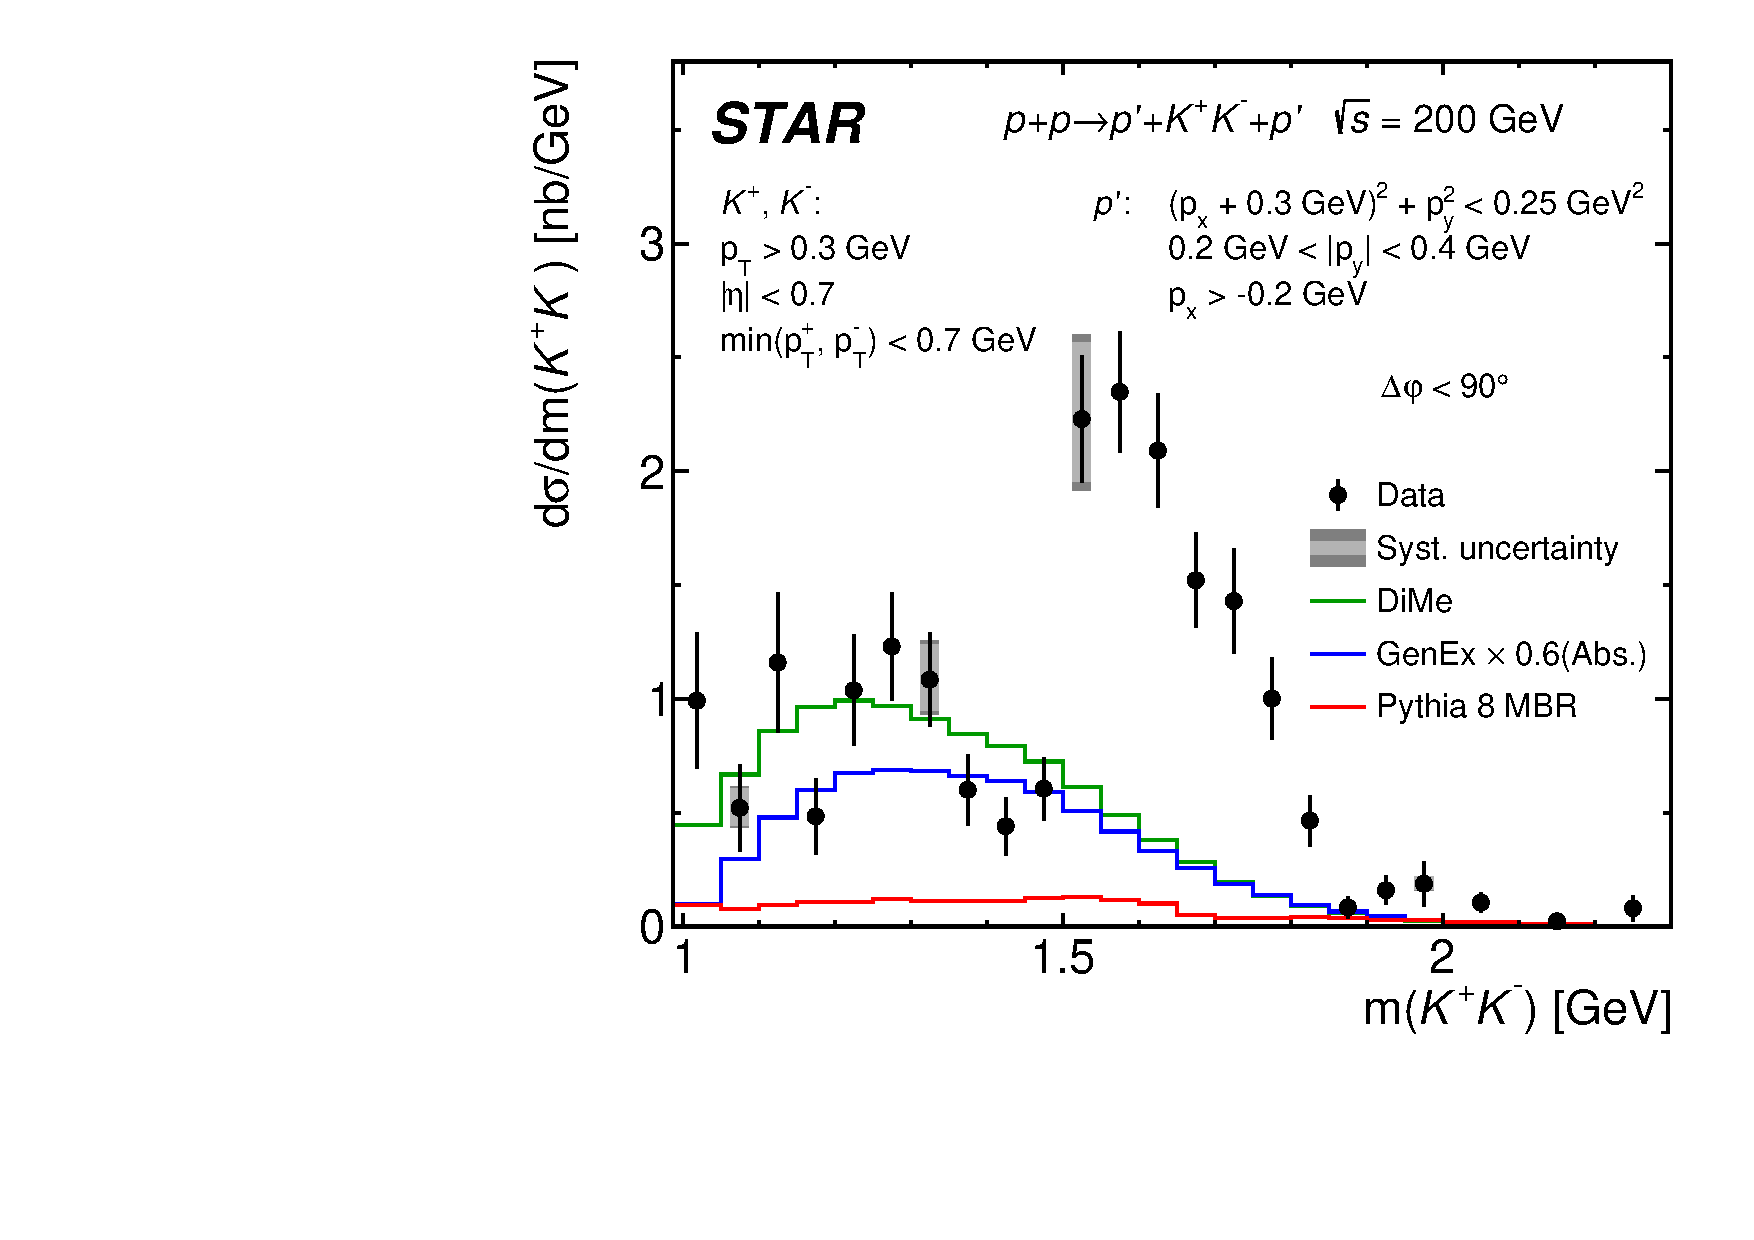
\includegraphics[width=.46\textwidth,page=1]{graphics/physicsResults/FinalResult_InvMass_DeltaPhiBin1_kaon.pdf}
\hfill
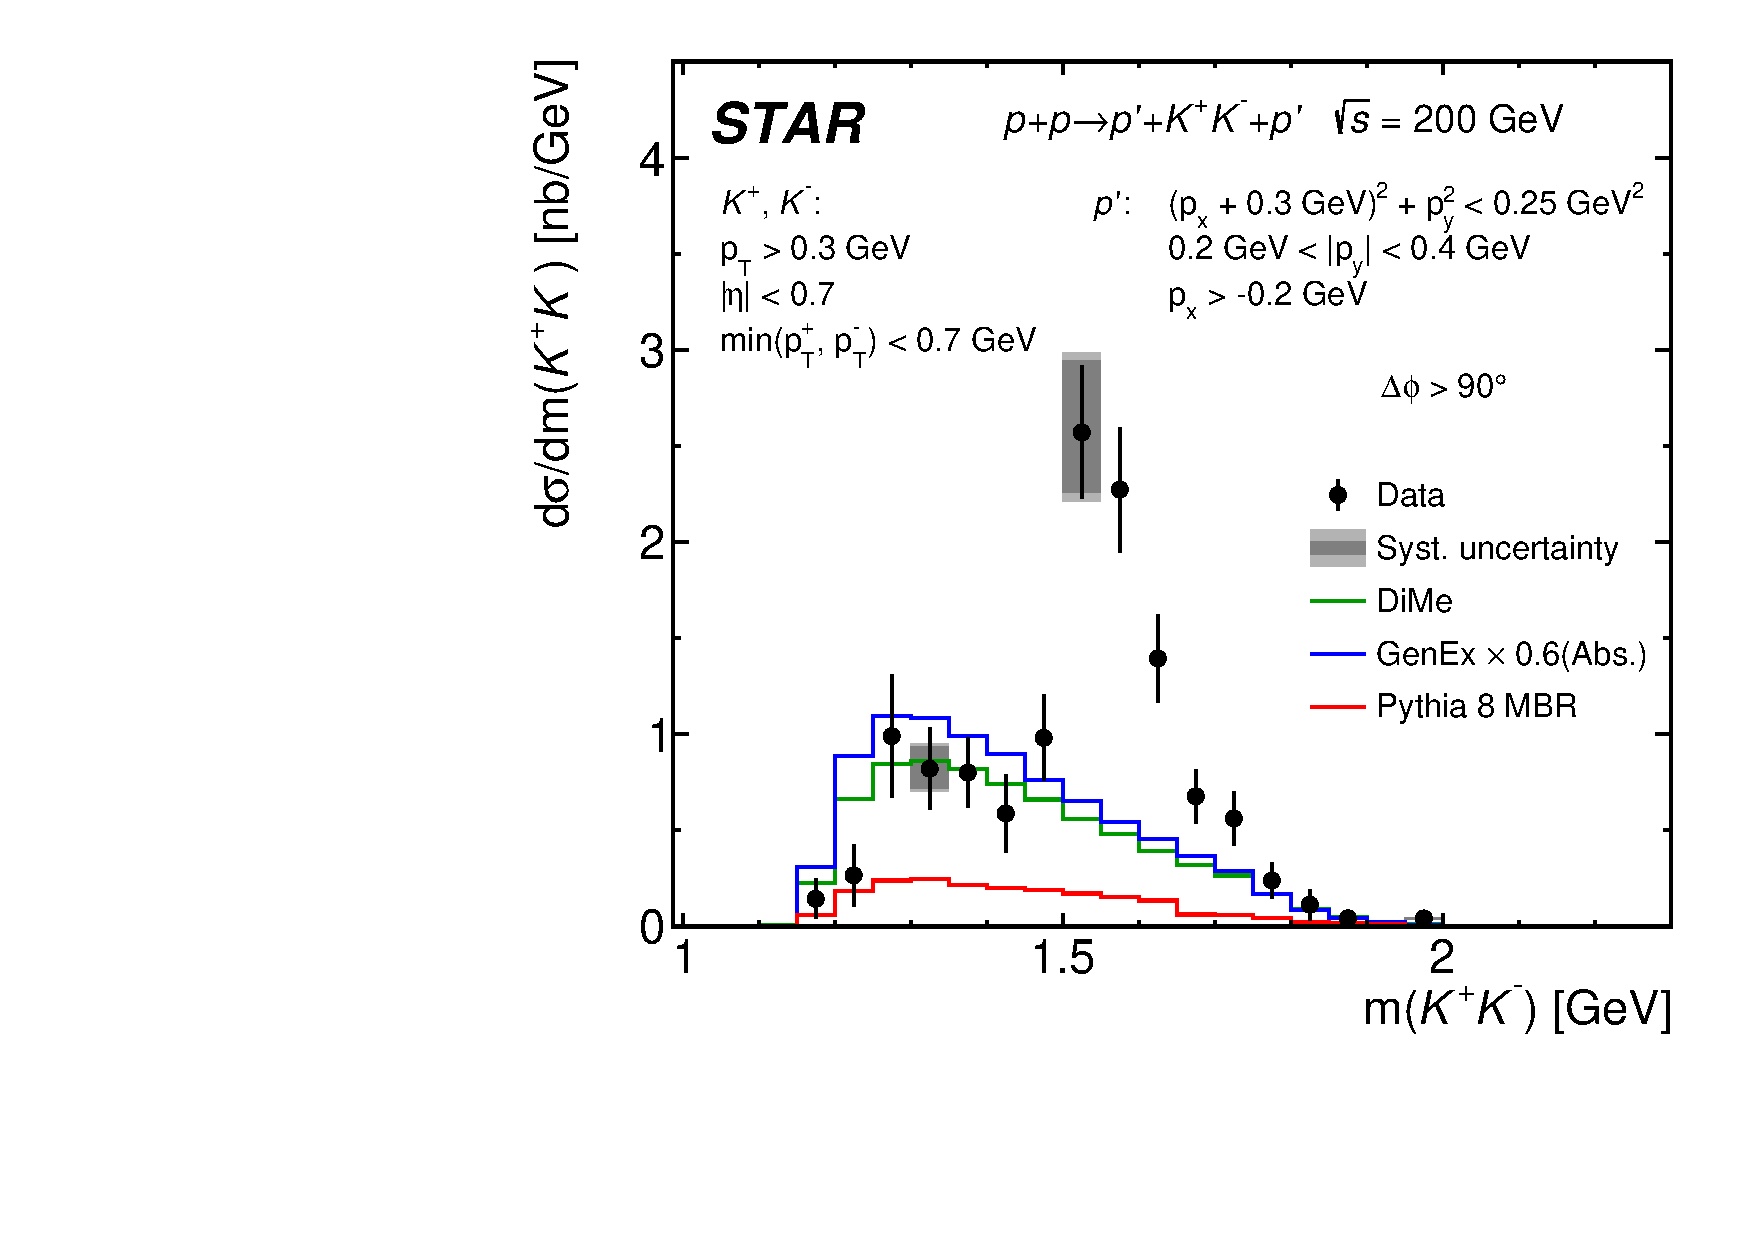
\includegraphics[width=.46\textwidth,page=1]{graphics/physicsResults/FinalResult_InvMass_DeltaPhiBin2_kaon.pdf}
\hspace*{5pt}
\newline
\hspace*{5pt}
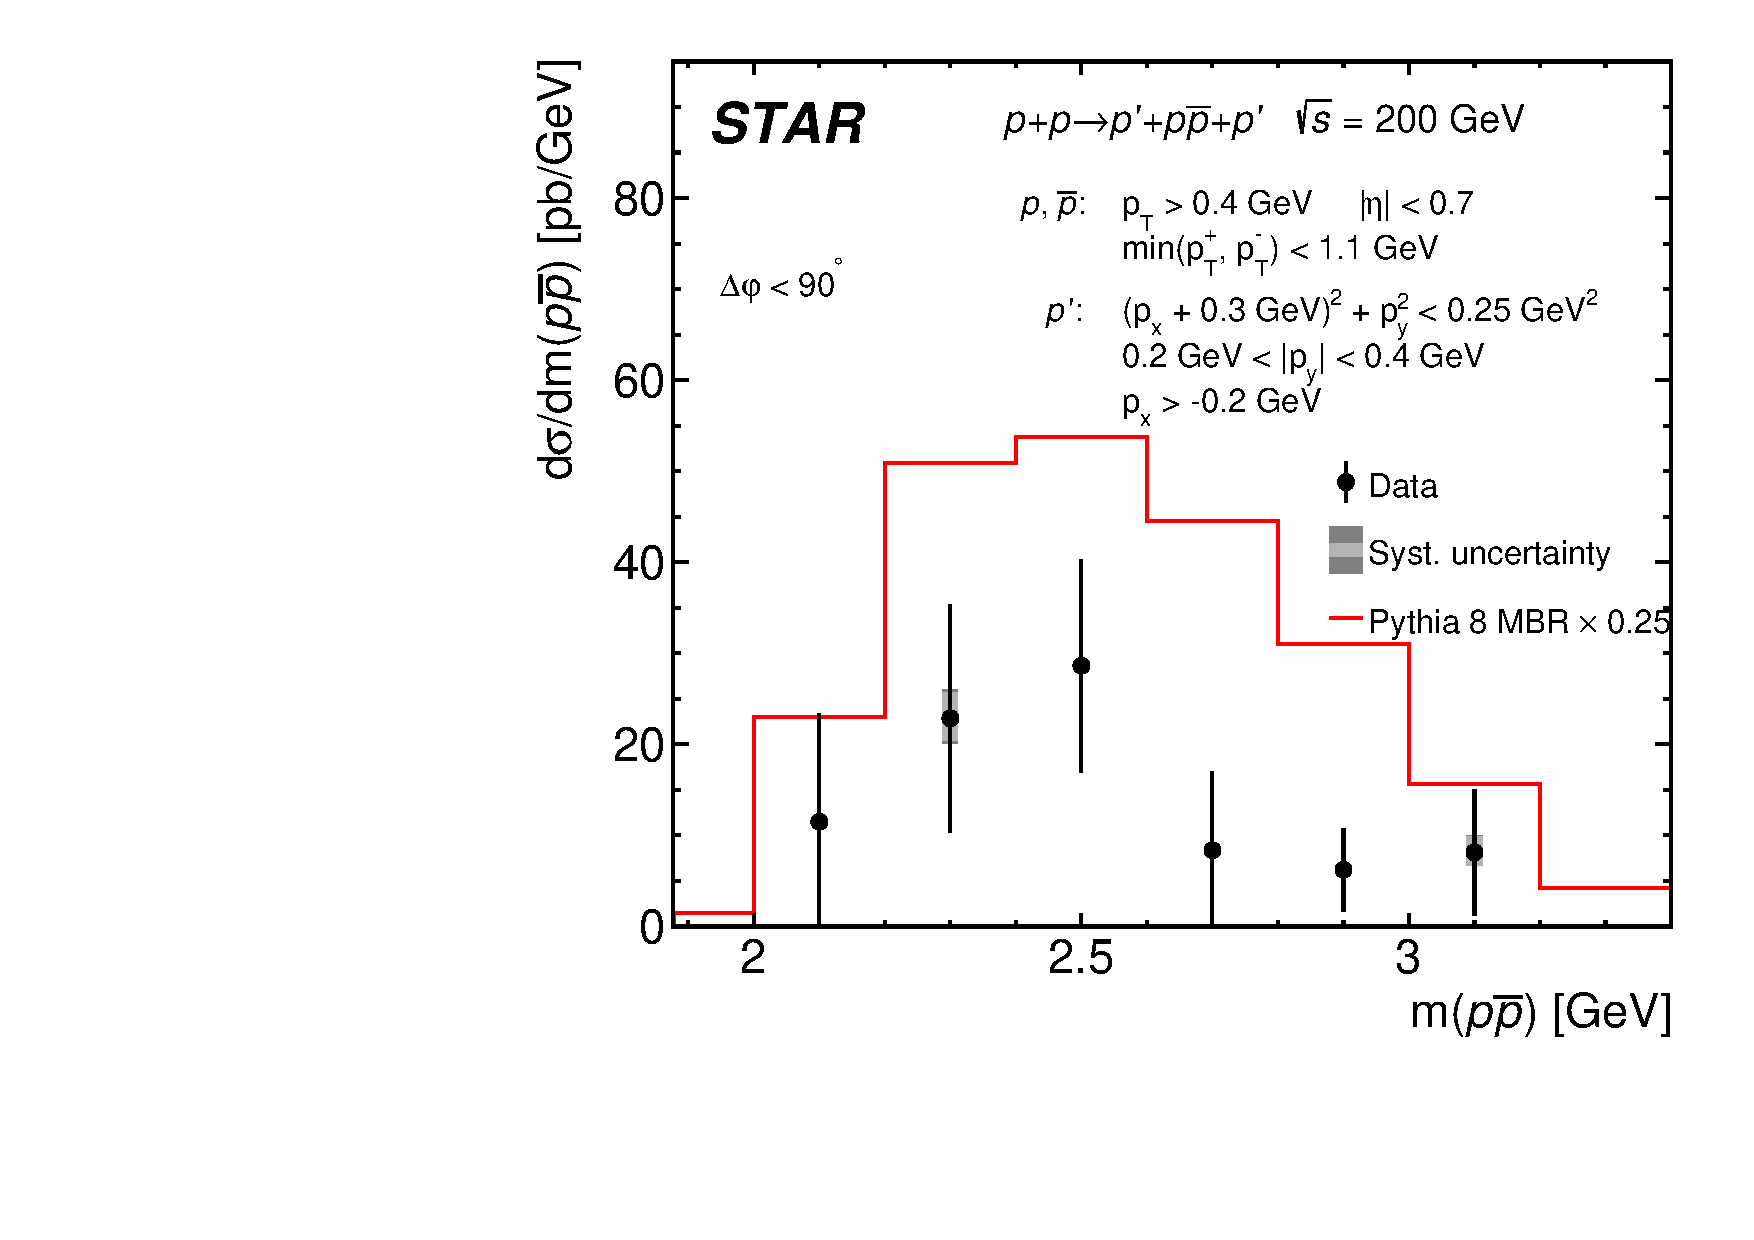
\includegraphics[width=.46\textwidth,page=1]{graphics/physicsResults/FinalResult_InvMass_DeltaPhiBin1_proton.pdf}
\hfill
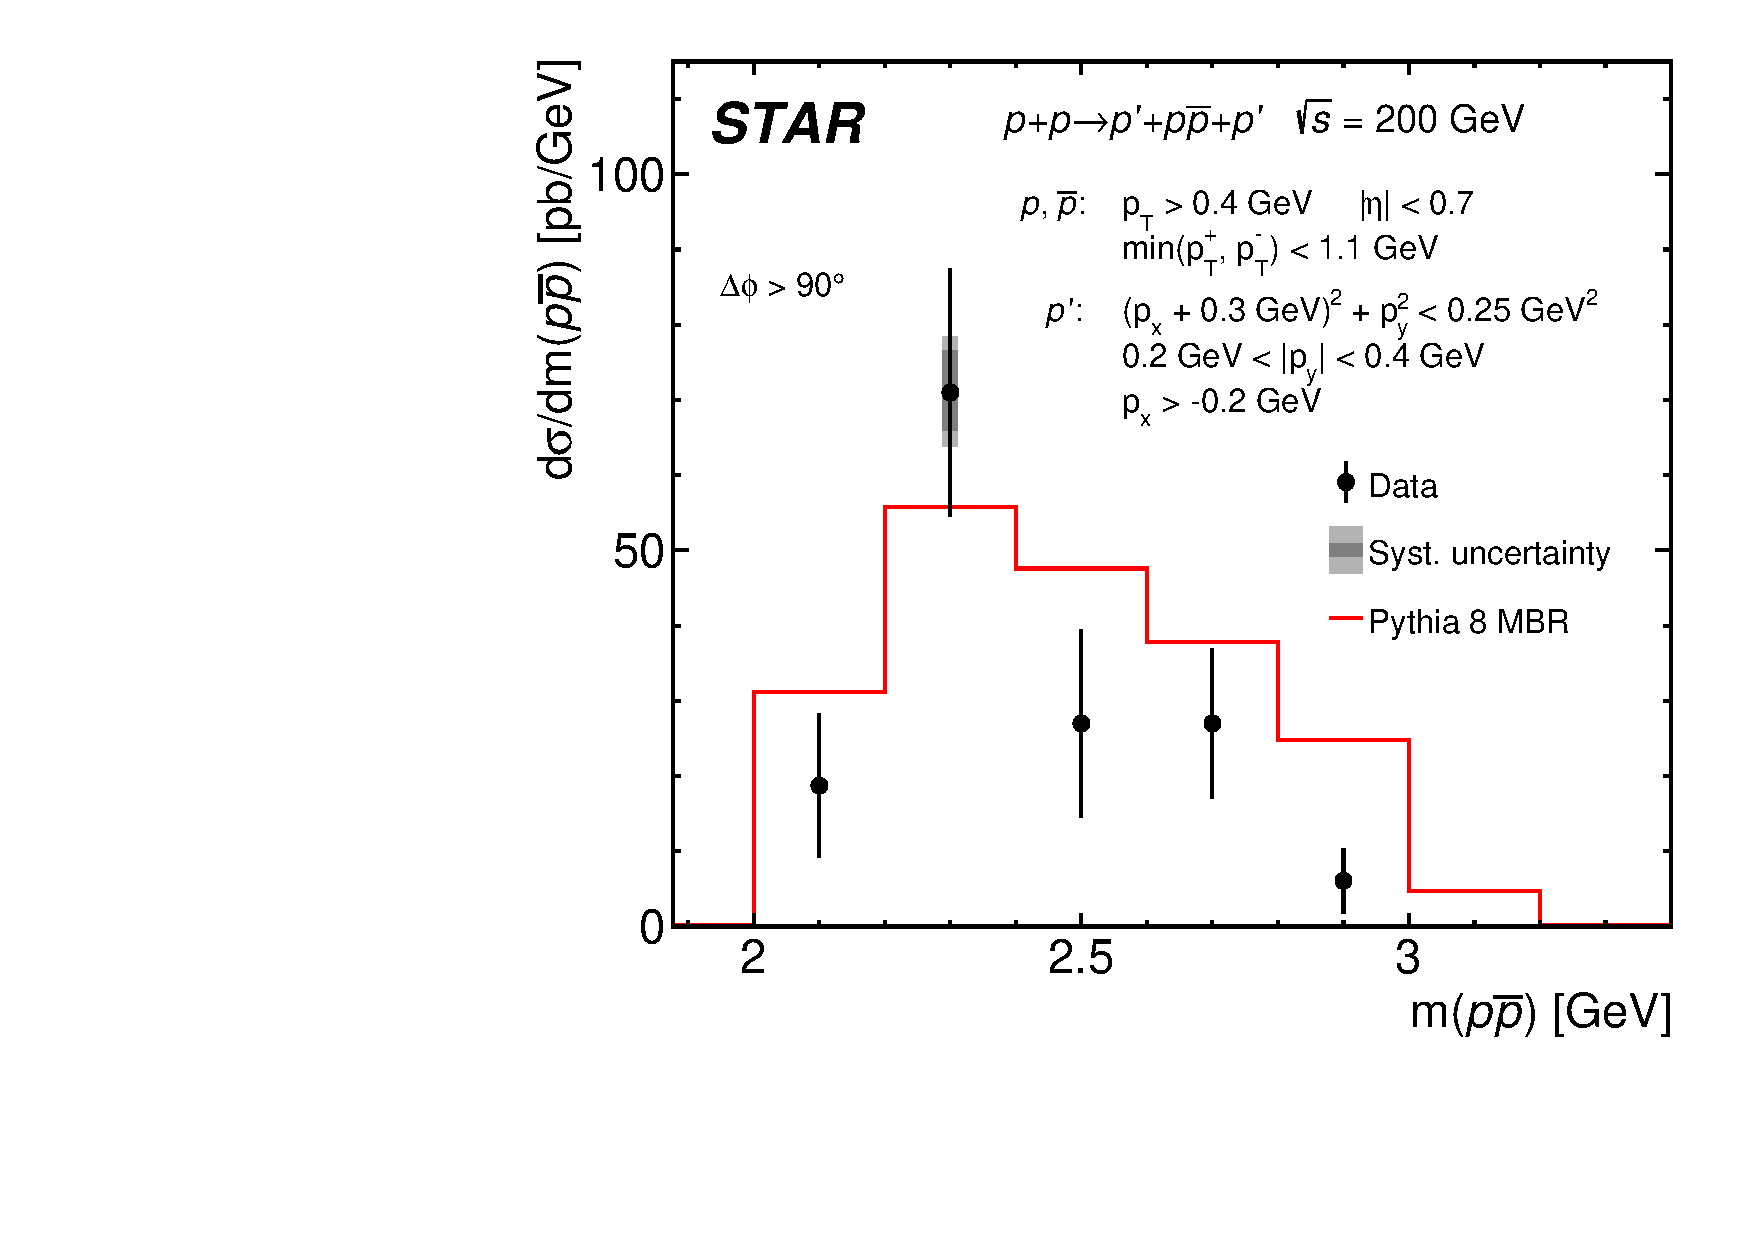
\includegraphics[width=.46\textwidth,page=1]{graphics/physicsResults/FinalResult_InvMass_DeltaPhiBin2_proton.pdf}
\hspace*{5pt}
%
\caption{Differential cross sections for CEP of charged particle pairs $\pi^+\pi^-$ (top), $K^+K^-$ (middle) and $p\bar{p}$ (bottom) as a function of the invariant mass of the pair in two $\Delta\phi$ regions: $\Delta\phi<90$ degree (left column) and $\Delta\phi>90$ degree (right column) measured in the fiducial region explained on the plots. Data are shown as solid points with error bars representing the statistical uncertainties. The typical systematic uncertainties are shown as gray boxes for only few data points as they are almost fully correlated between neighboring bins. Predictions from MC models GenEx, DiMe and MBR are shown as histograms.}
\label{results_3}
\end{figure}



{
\renewcommand{\arraystretch}{1.5}
\begin{table}[]\centering
\begin{tabular}{cc c c}
~ & ~ & \multicolumn{2}{c}{$\bm{ \sigma_{\text{\bf{fid}}} \pm \delta_{\text{\bf{stat}}} \pm \delta_{\text{\bf{syst}}}}$} \\
 \bf{PID} & \bf{unit} & $\bm{\Delta\varphi<90^{\circ}}$ & $\bm{\Delta\varphi>90^{\circ}}$ \\ \hline\hline
 $\bm{\pi^{+}\pi^{-}}$ & \bf{nb} & $38.1\pm0.2^{+4.3}_{-4.0}$ & $18.4\pm0.1^{+2.0}_{-1.8}$ \\ %\hline
 $\bm{K^{+}K^{-}}$ & \bf{pb} & $976\pm46^{+156}_{-140}$ & $533\pm33^{+84}_{-76}$ \\ %\hline
 $\bm{p\bar{p}}$ & \bf{pb} & $17.7\pm3.6^{+2.3}_{-2.1}$ & $31.5\pm5.4^{+3.9}_{-3.6}$\\ %\hline%\hline
\end{tabular}
\caption{Integrated fiducial cross sections for CEP of $\pi^{+}\pi^{-}$, $K^{+}K^{-}$ and $p\bar{p}$ pairs in two ranges of azimuthal angle difference $\Delta\varphi$ between forward scattered protons. Statistical and systematic uncertainties are provided for each cross section.}\label{tab:xSec}
\end{table}
}


% %
% \FloatBarrier
% %
% Such correlation between resonances seen in mass spectrum and azimuthal angle between outgoing protons indicates factorization breaking between the two proton vertices. In the range $\Delta\phi<$ 90 degrees the DiMe model well describes both normalization and shape of mass spectrum at $m(\pi^+\pi^-)<$ 0.5 GeV.
% %
% In case of the cross section for CEP of $K^+K^-$ pairs the data do not show any significant asymmetry except possible widening
% of the peak at $f_2^\prime(1520)$ in the region $\Delta\phi<90$ degrees which may indicate an enhancement of additional resonances around 1.7~GeV in this configuration.
% %
% In case of the cross section for CEP of $p\bar{p}$ pairs data do not show any significant asymmetry except possible enhancement in the $2.2-2.4$ mass range for the $\Delta\phi>90$ degrees region.\\
% %
% \indent
% Due to high statistics of the two-pion sample it is possible to study the CEP of $\pi^+\pi^-$ pairs in more detail.
% Figure~\ref{results_4} shows the differential cross sections for CEP of $\pi^+\pi^-$ pairs as a function of the pair rapidity (left column), $\Delta\phi$ (middle column) and $|t_1+t_2|$ (right column) in three characteristic ranges of the invariant mass of the pair: $m(\pi^+\pi^-)<1.0$ GeV (mainly non-resonant production), $1.0< m(\pi^+\pi^-) <1.5$ GeV ($f_2(1270)$ mass range) and $m(\pi^+\pi^-)>1.5$ GeV (higher invariant masses).\\
% %
% \noindent
% Figure~\ref{results_4} shows the differential cross sections for CEP of different particle species pairs as a function of the pair rapidity (left column), of the difference of forward protons azimuthal angles (middle column) and of the sum of squares of the four-momenta transfers at the proton vertices (right column), for the three invariant mass ranges. In the case of the cross section $d\sigma/dy$ all models agree in shape with data in all three mass ranges except for the GenEx and DiMe predictions in the highest mass range where predictions is narrower.
% 
% Strong suppression of the fiducial cross section close to $90^\circ$ is due to the STAR RP acceptance while asymmetry $0^\circ$ vs. $180^\circ$ in the lowest mass region is due to the STAR TPC acceptance. $\Delta\phi$ distribution is sensitive to absorption  which are treated fully differentialy in DiMe generator and only on average in GenEx. This is consistent with generally better agreement between data and DiMe expectations except $f_2(1270)$ mass region. MBR model predicts symmetric $\Delta\phi$ distributions in all mass ranges which is not supported by the data.
% 
% The slope of the cross section as the function of $|t_1+t_2|$ is less steep in the $f_2(1270)$ mass region compared to other mass regions. In the low mass region the DiMe prediction has steeper slope compared to data.\\
%
\begin{figure}[h]
\centering
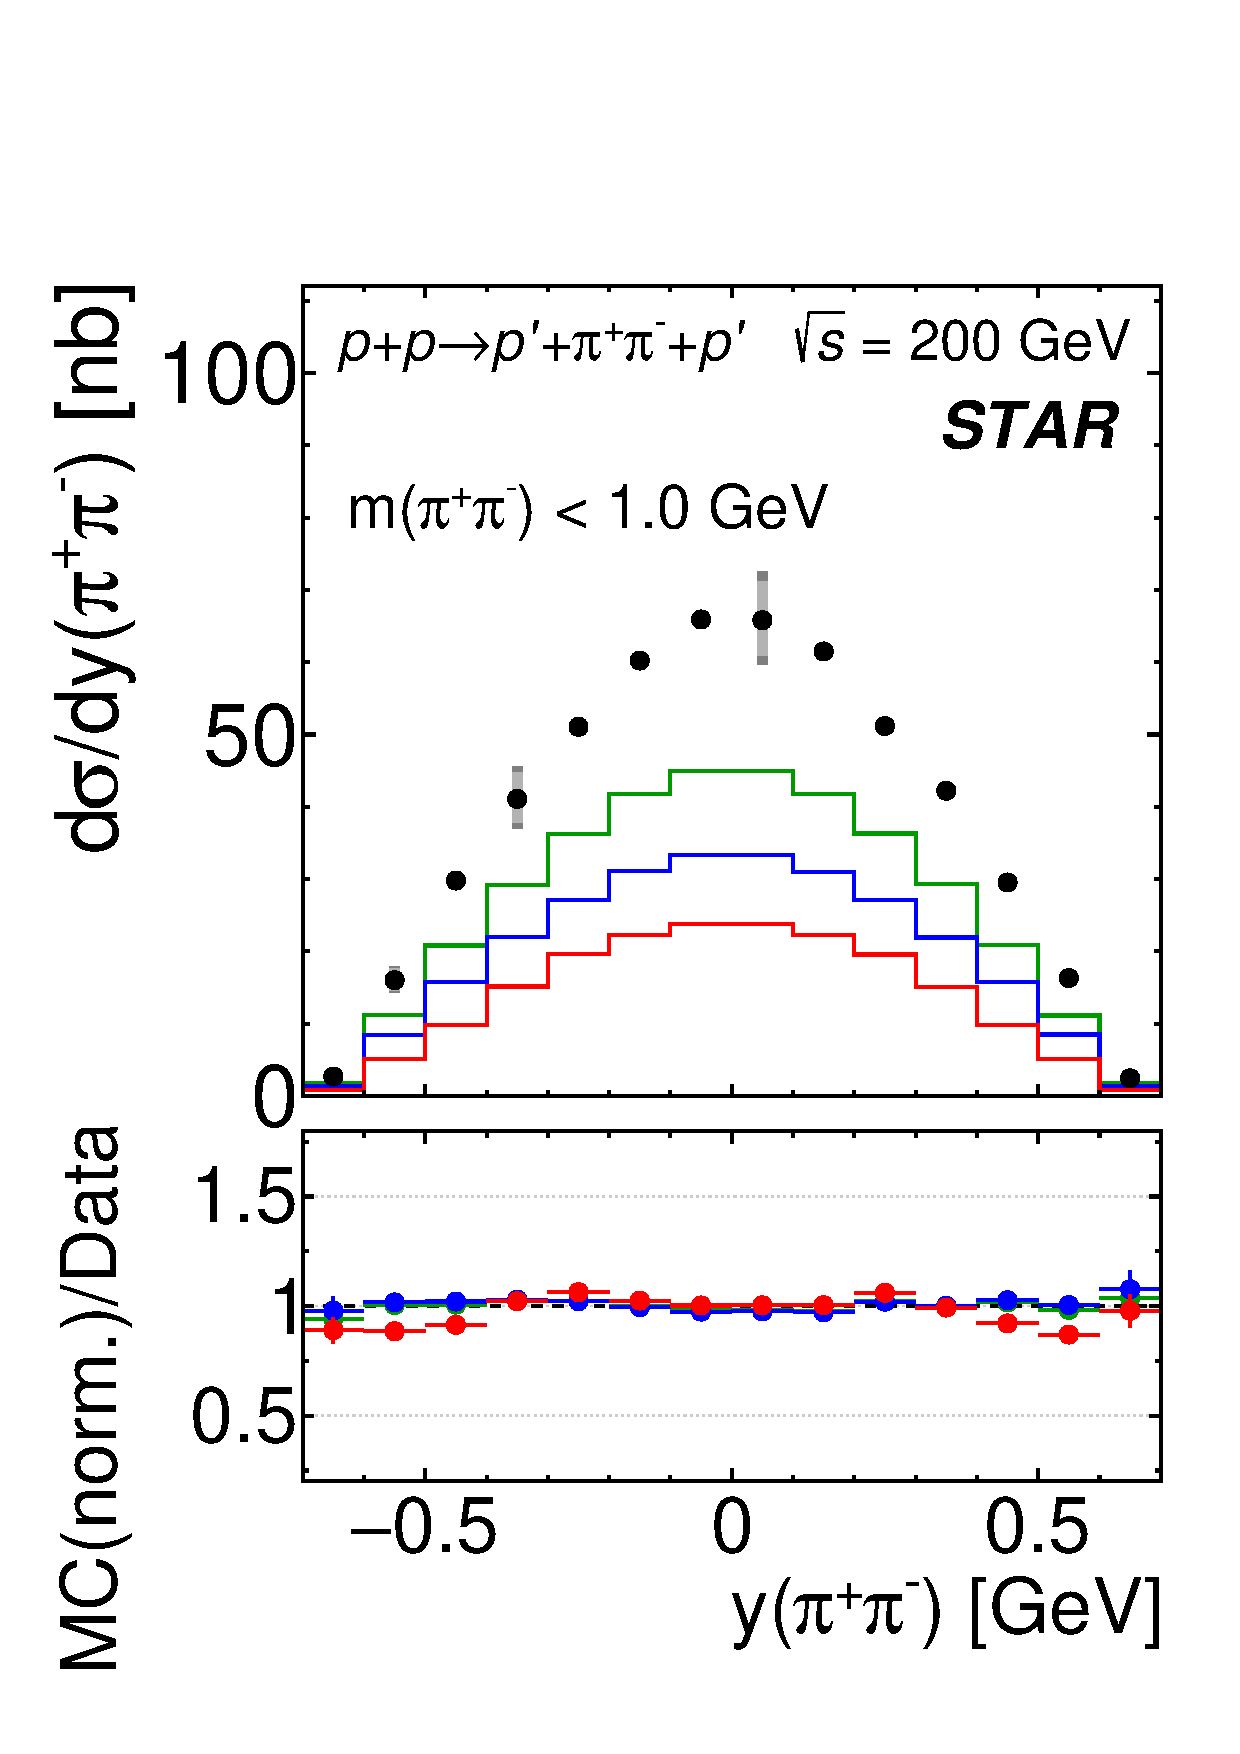
\includegraphics[width=.31\textwidth,page=1]{graphics/physicsResults/Ratio_FinalResult_Rapidity_pion_MassBin_1.pdf}
\hfill
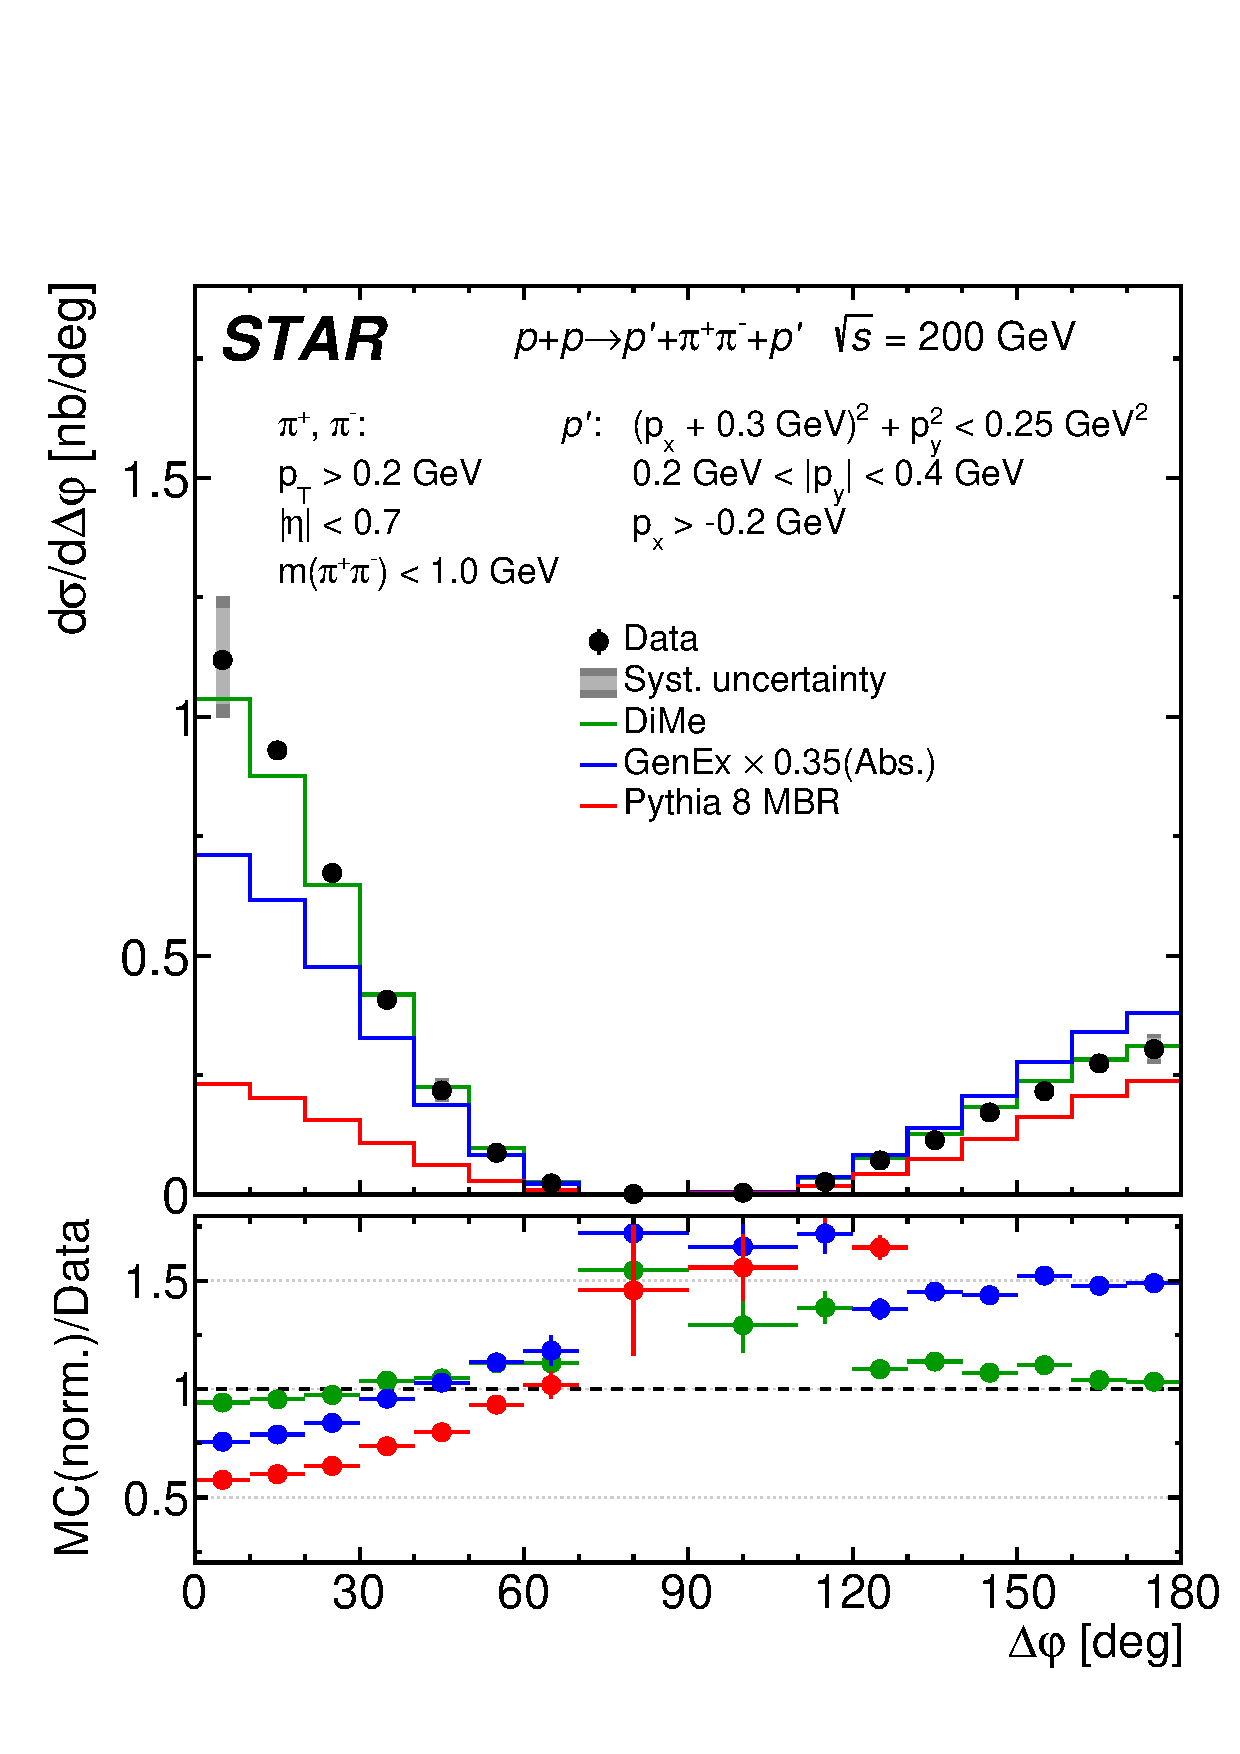
\includegraphics[width=.31\textwidth,page=1]{graphics/physicsResults/Ratio_FinalResult_DeltaPhi_pion_MassBin_1.pdf}
\hfill
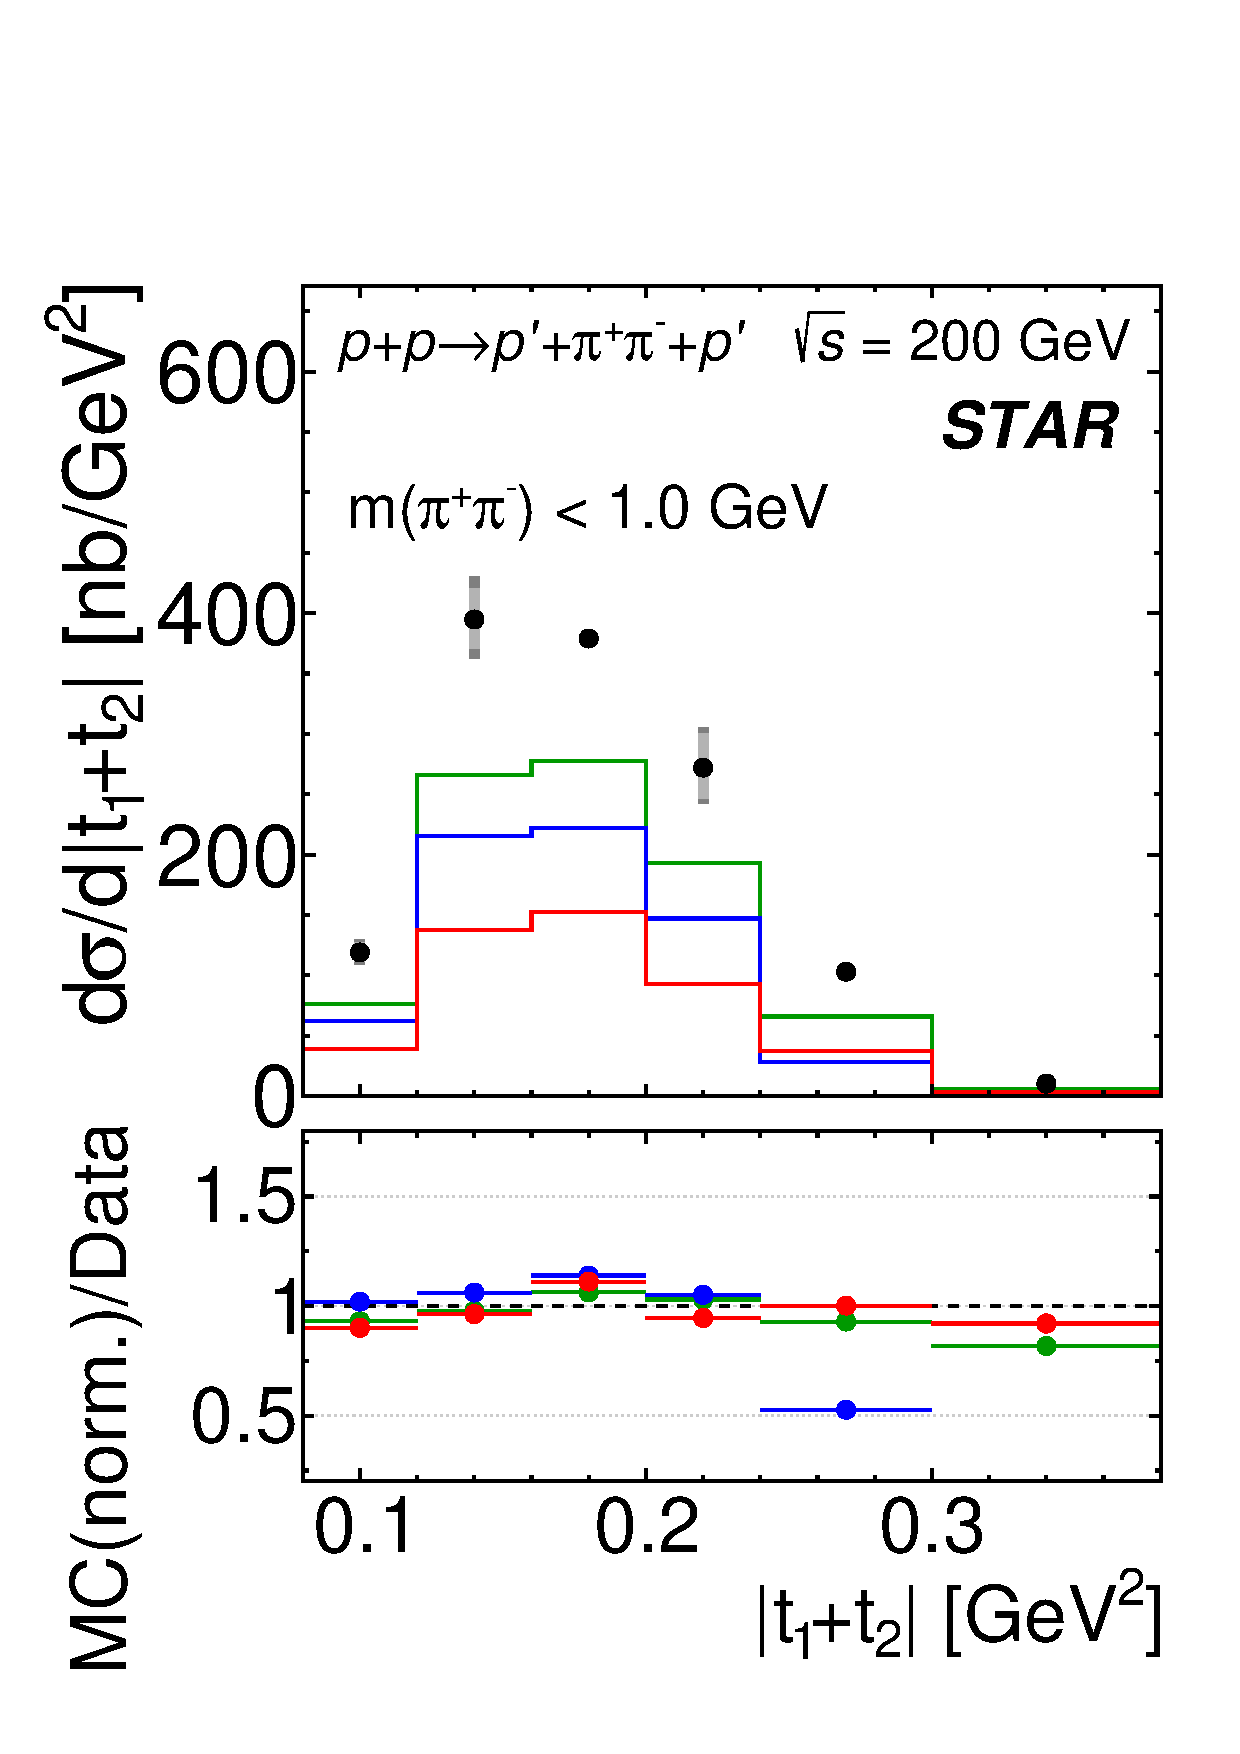
\includegraphics[width=.31\textwidth,page=1]{graphics/physicsResults/Ratio_FinalResult_MandelstamTSum_pion_MassBin_1.pdf}
\newline
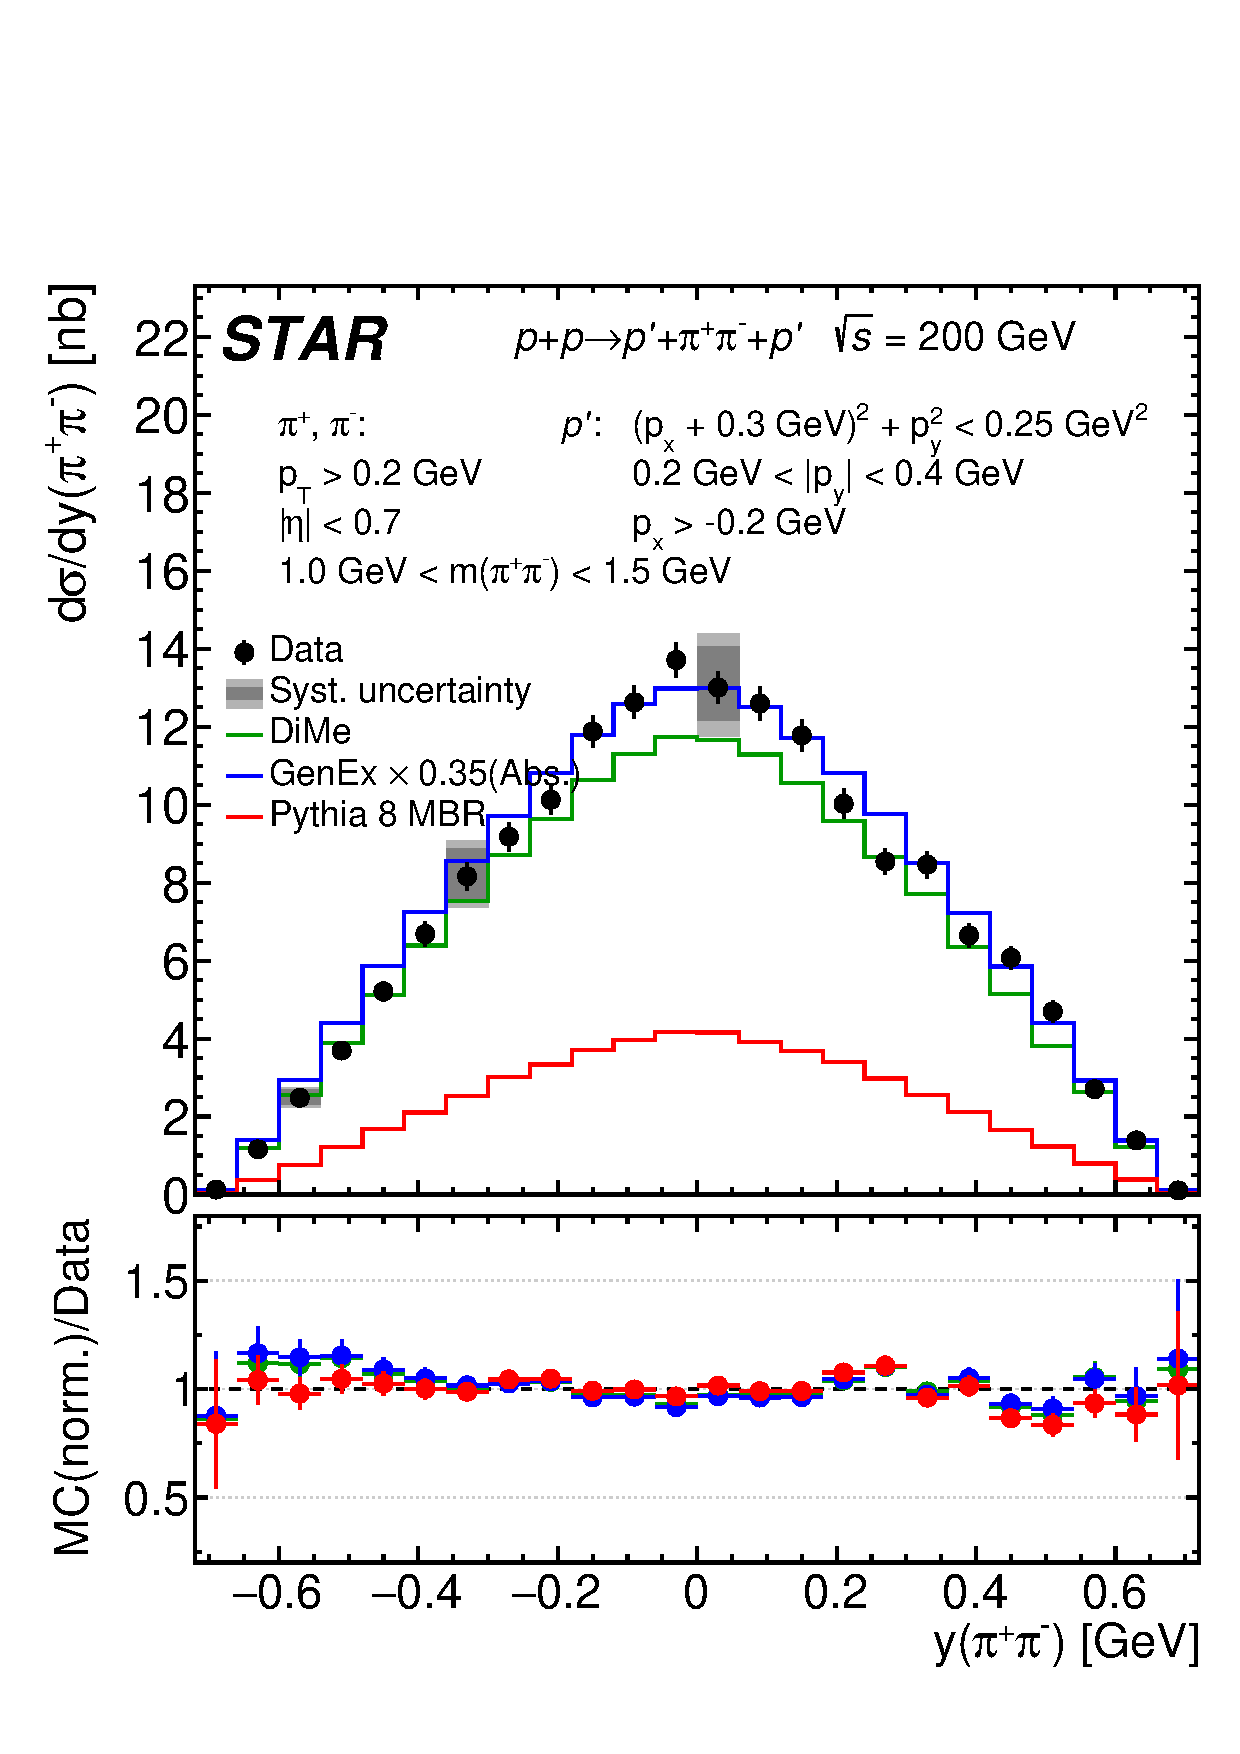
\includegraphics[width=.31\textwidth,page=1]{graphics/physicsResults/Ratio_FinalResult_Rapidity_pion_MassBin_2.pdf}
\hfill
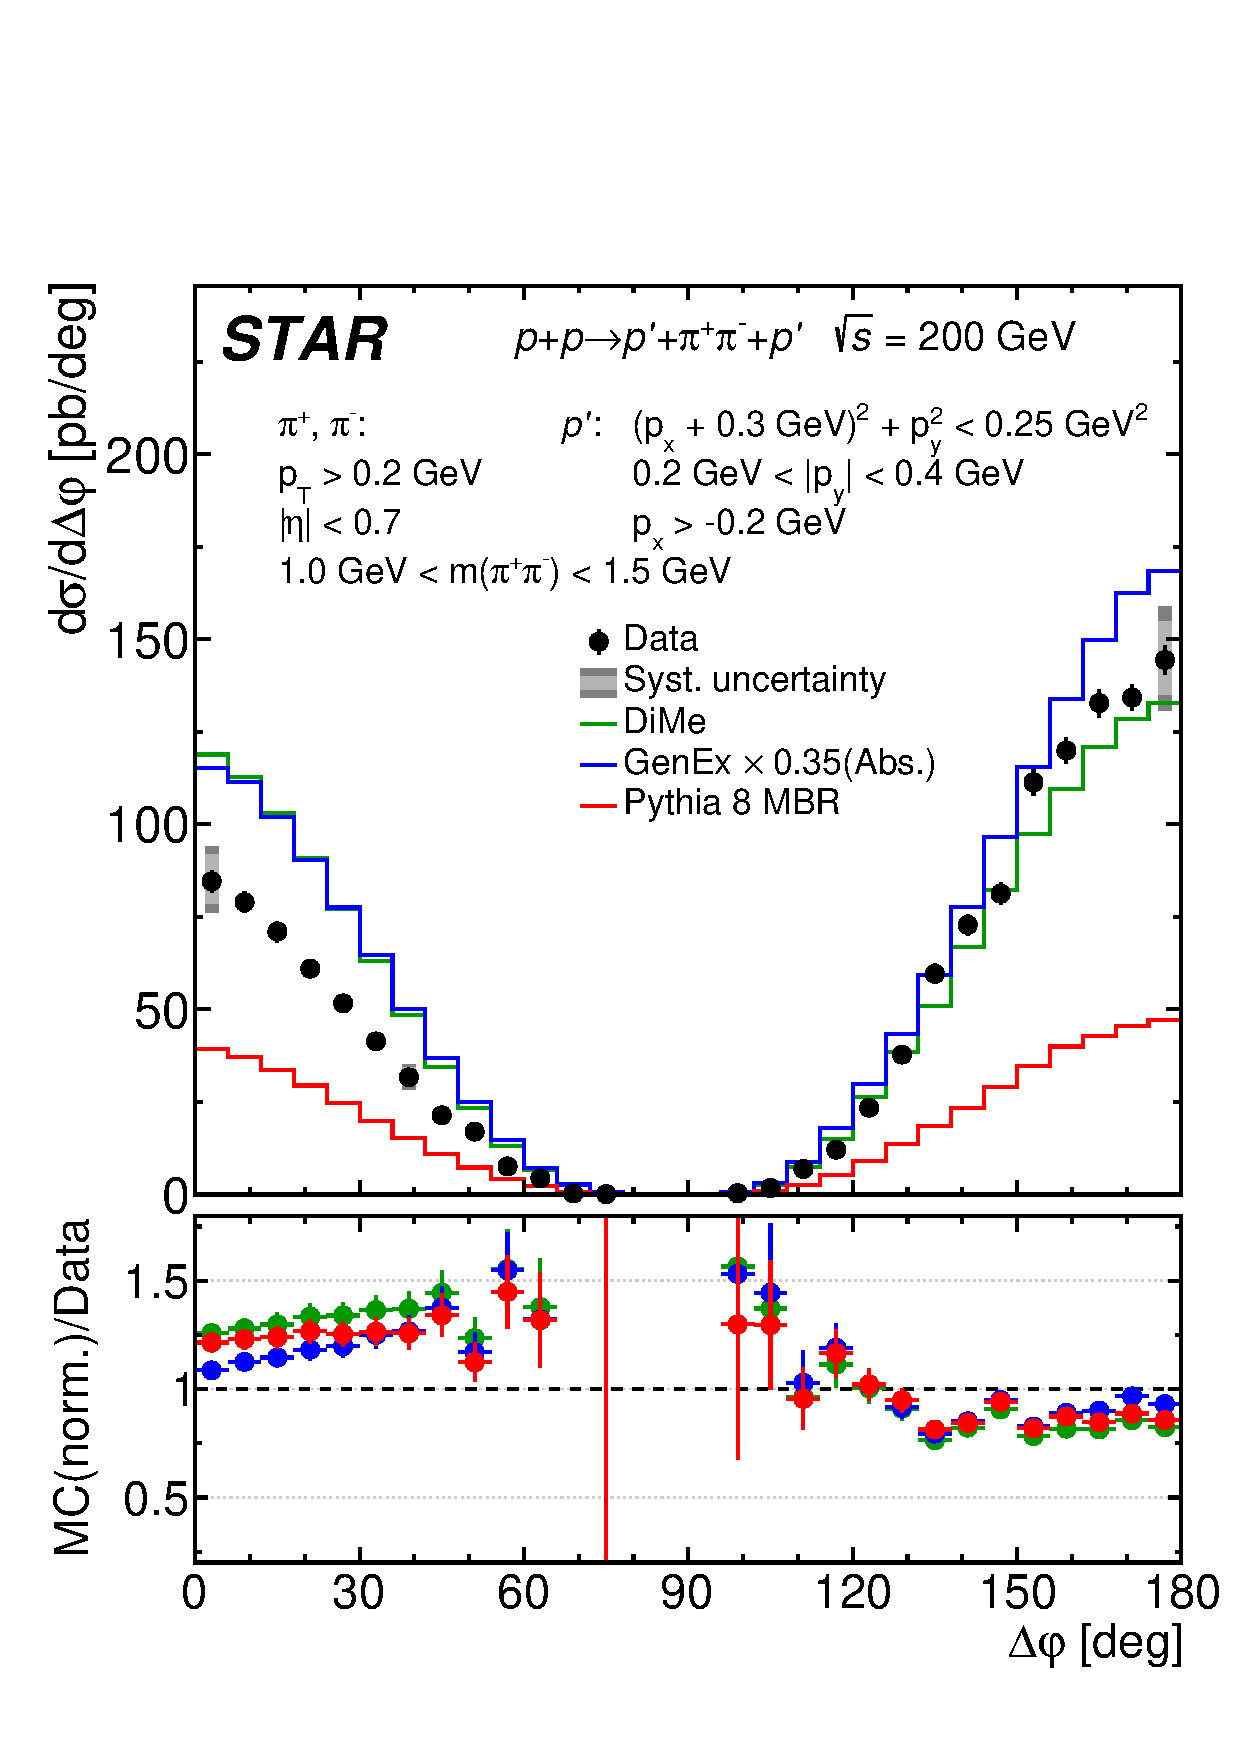
\includegraphics[width=.31\textwidth,page=1]{graphics/physicsResults/Ratio_FinalResult_DeltaPhi_pion_MassBin_2.pdf}
\hfill
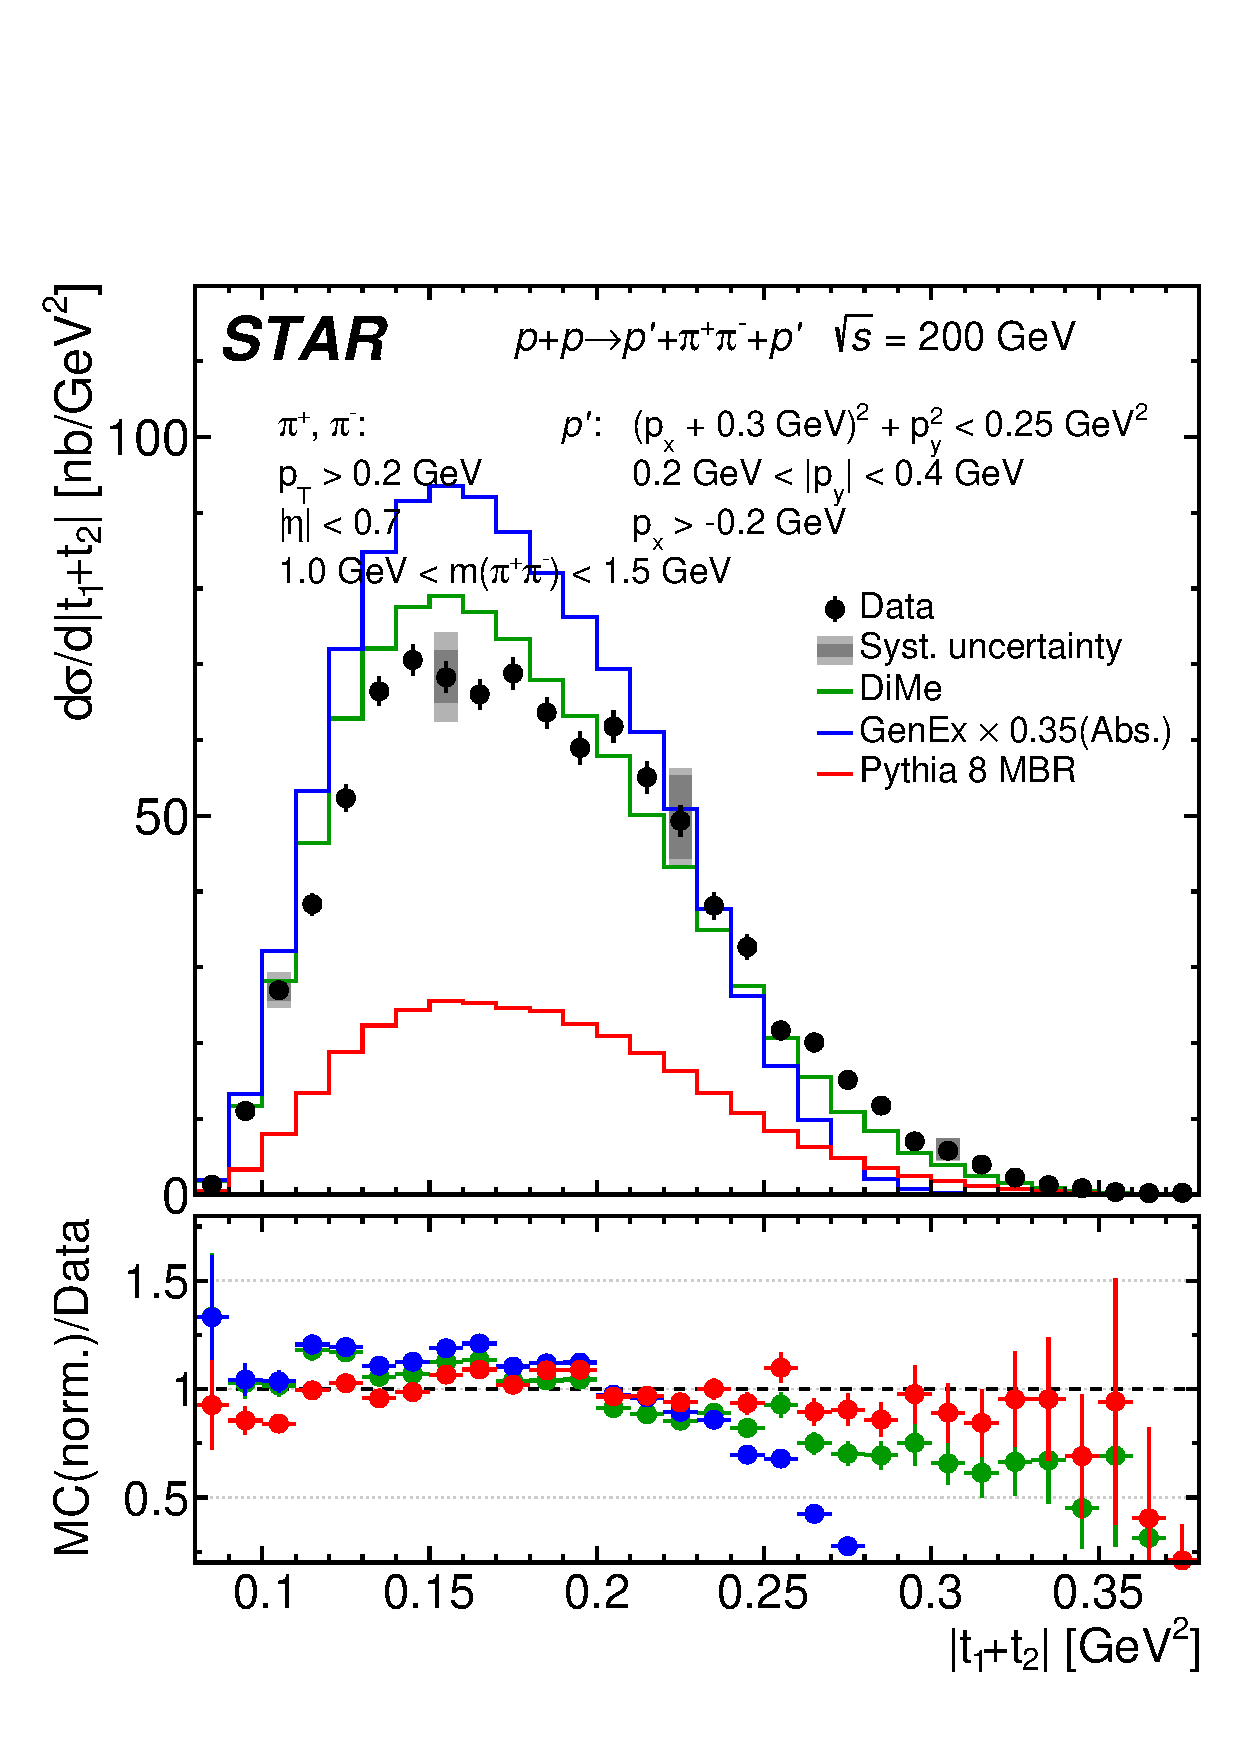
\includegraphics[width=.31\textwidth,page=1]{graphics/physicsResults/Ratio_FinalResult_MandelstamTSum_pion_MassBin_2.pdf}
\newline
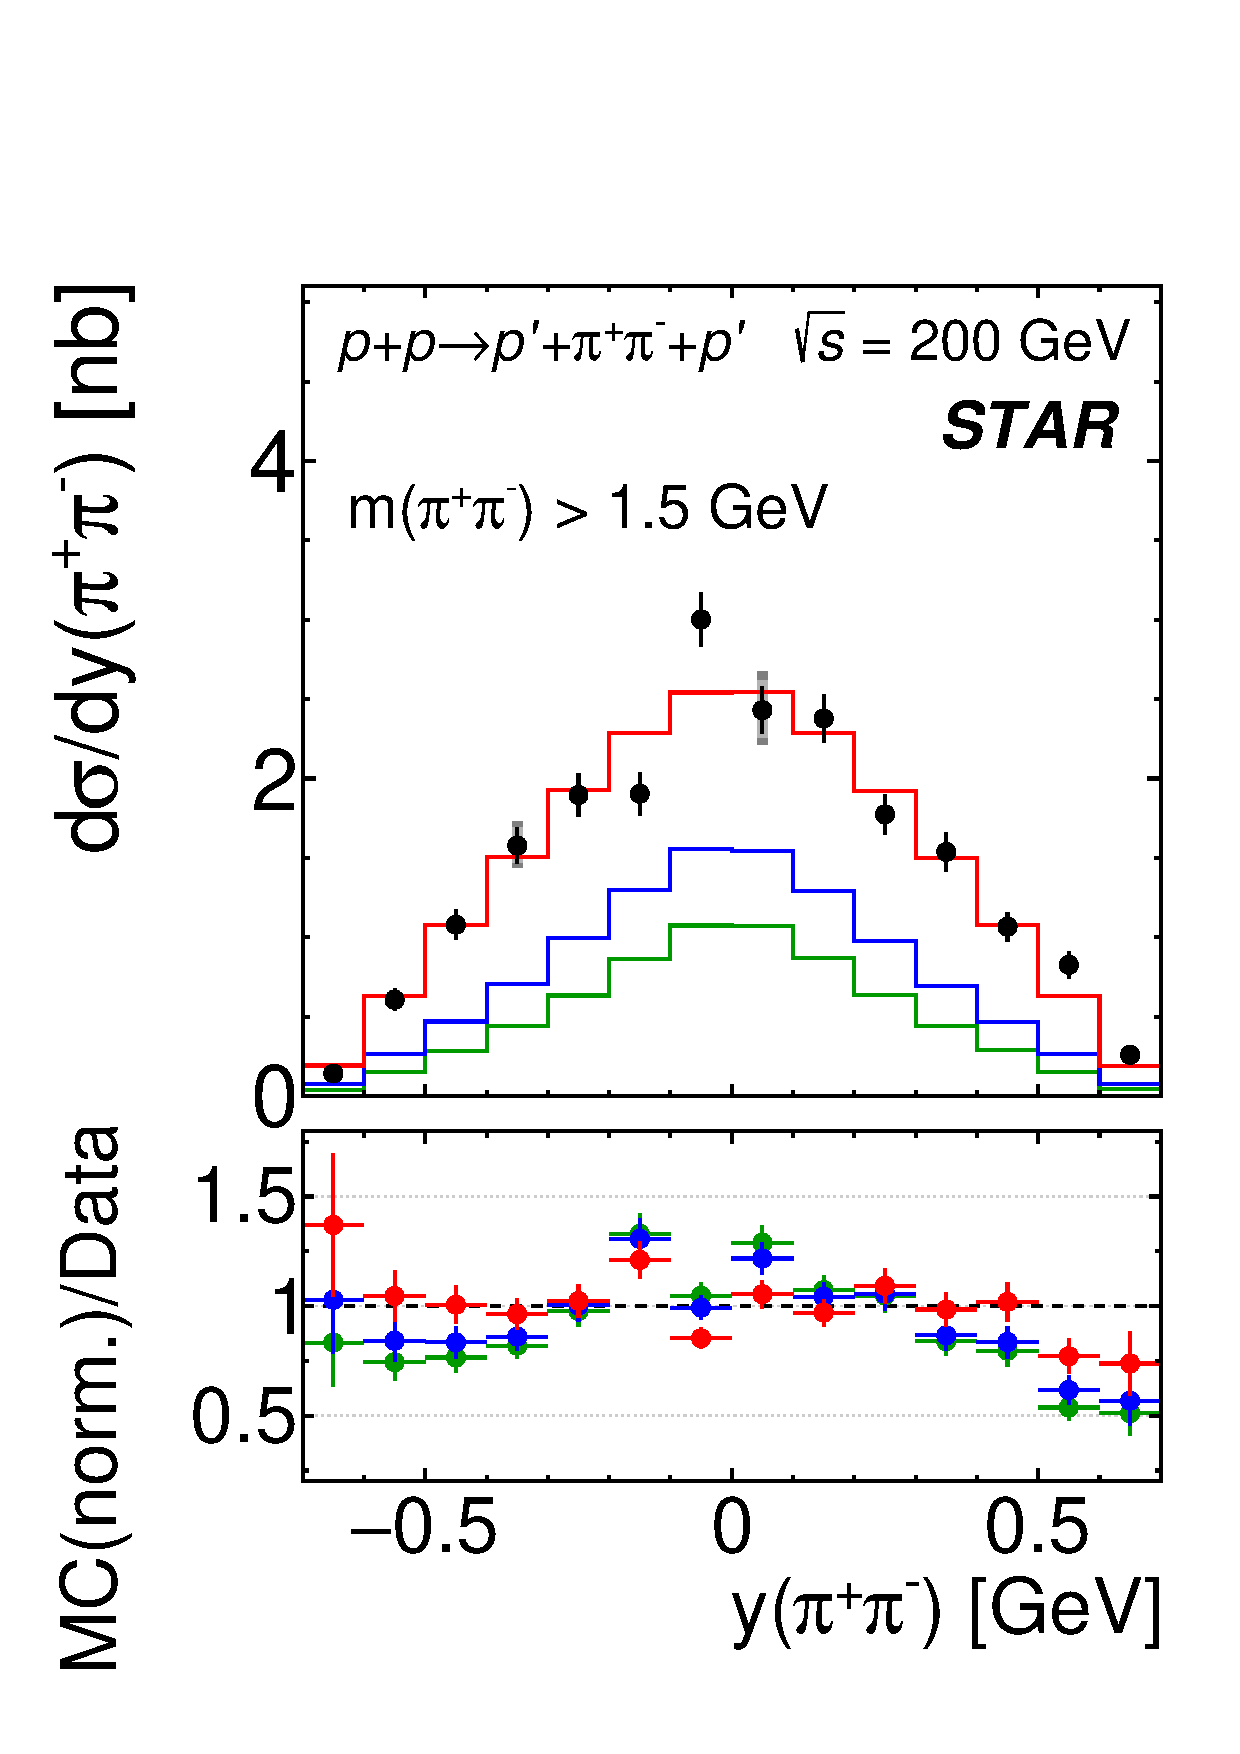
\includegraphics[width=.31\textwidth,page=1]{graphics/physicsResults/Ratio_FinalResult_Rapidity_pion_MassBin_3.pdf}
\hfill
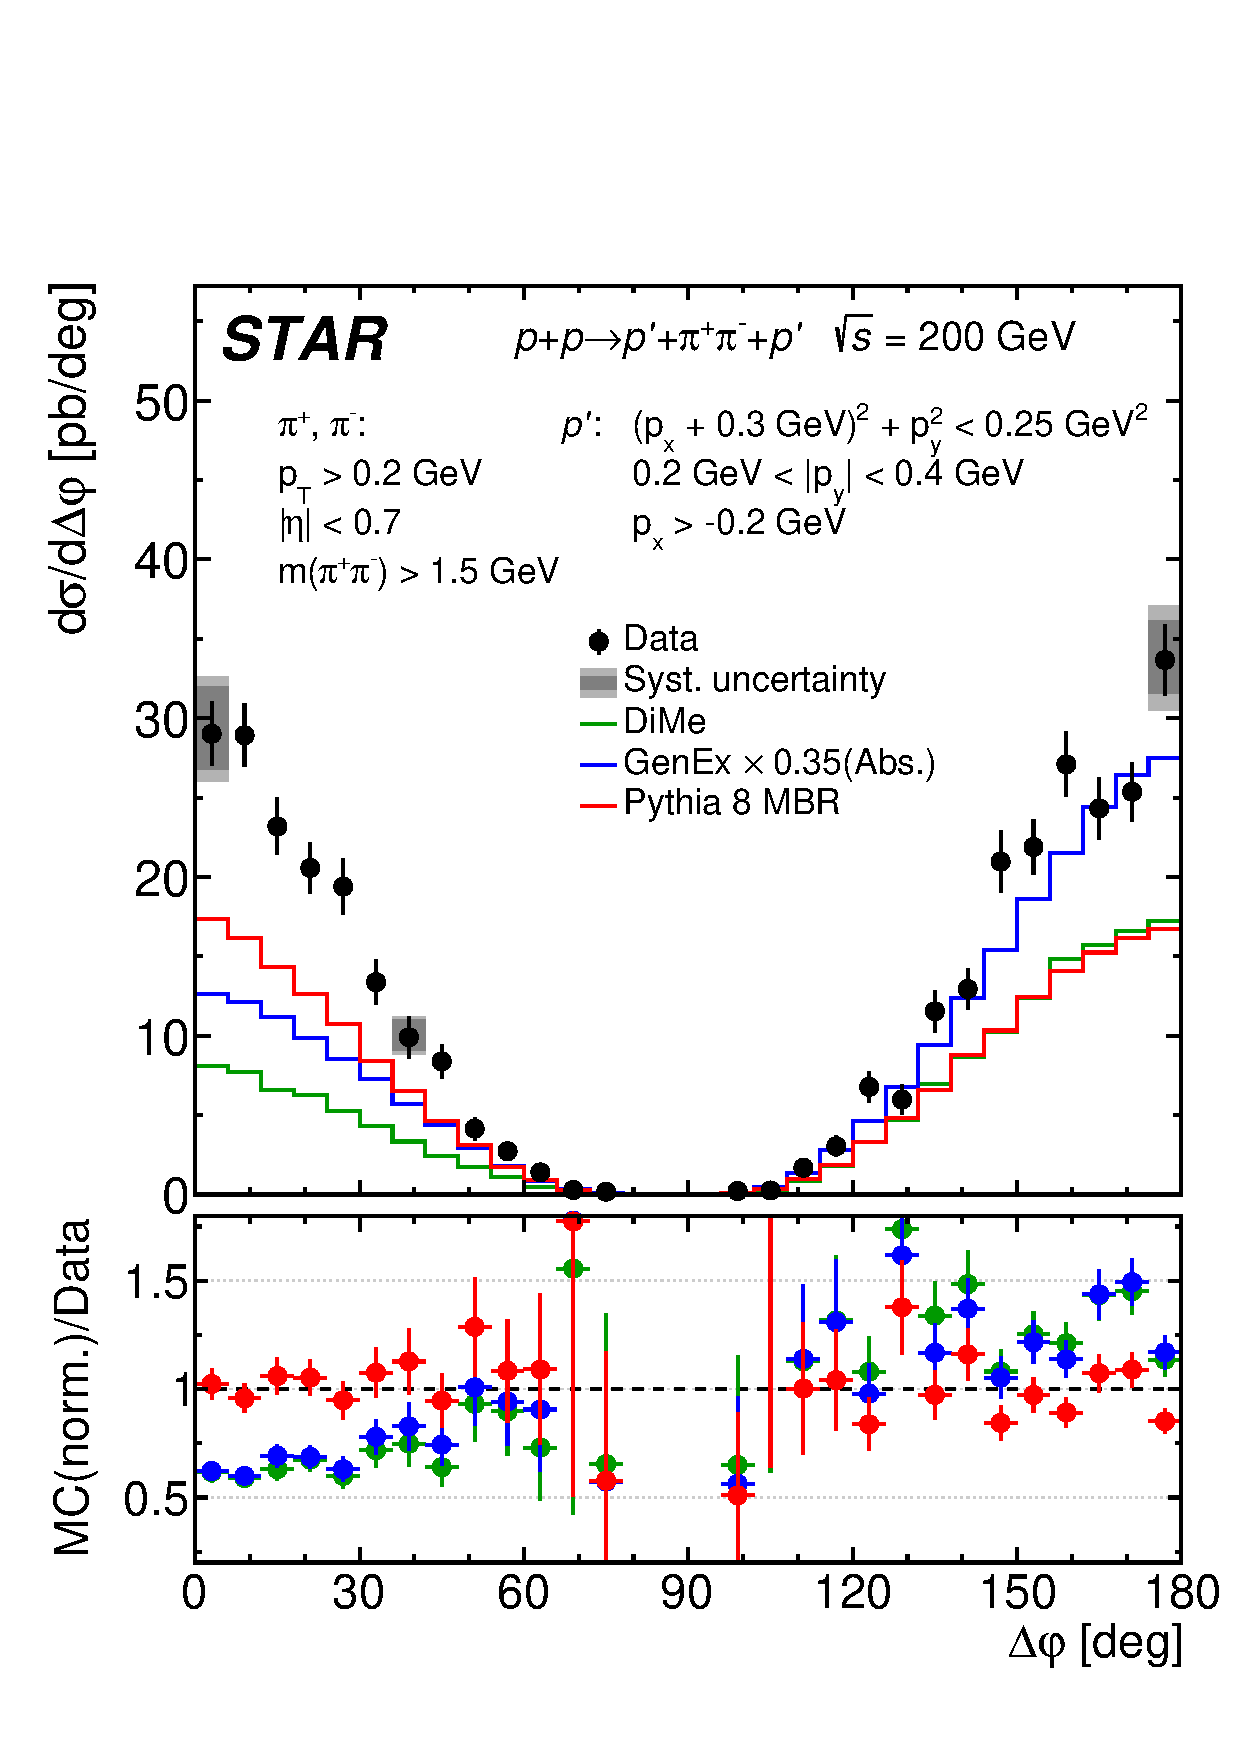
\includegraphics[width=.31\textwidth,page=1]{graphics/physicsResults/Ratio_FinalResult_DeltaPhi_pion_MassBin_3.pdf}
\hfill
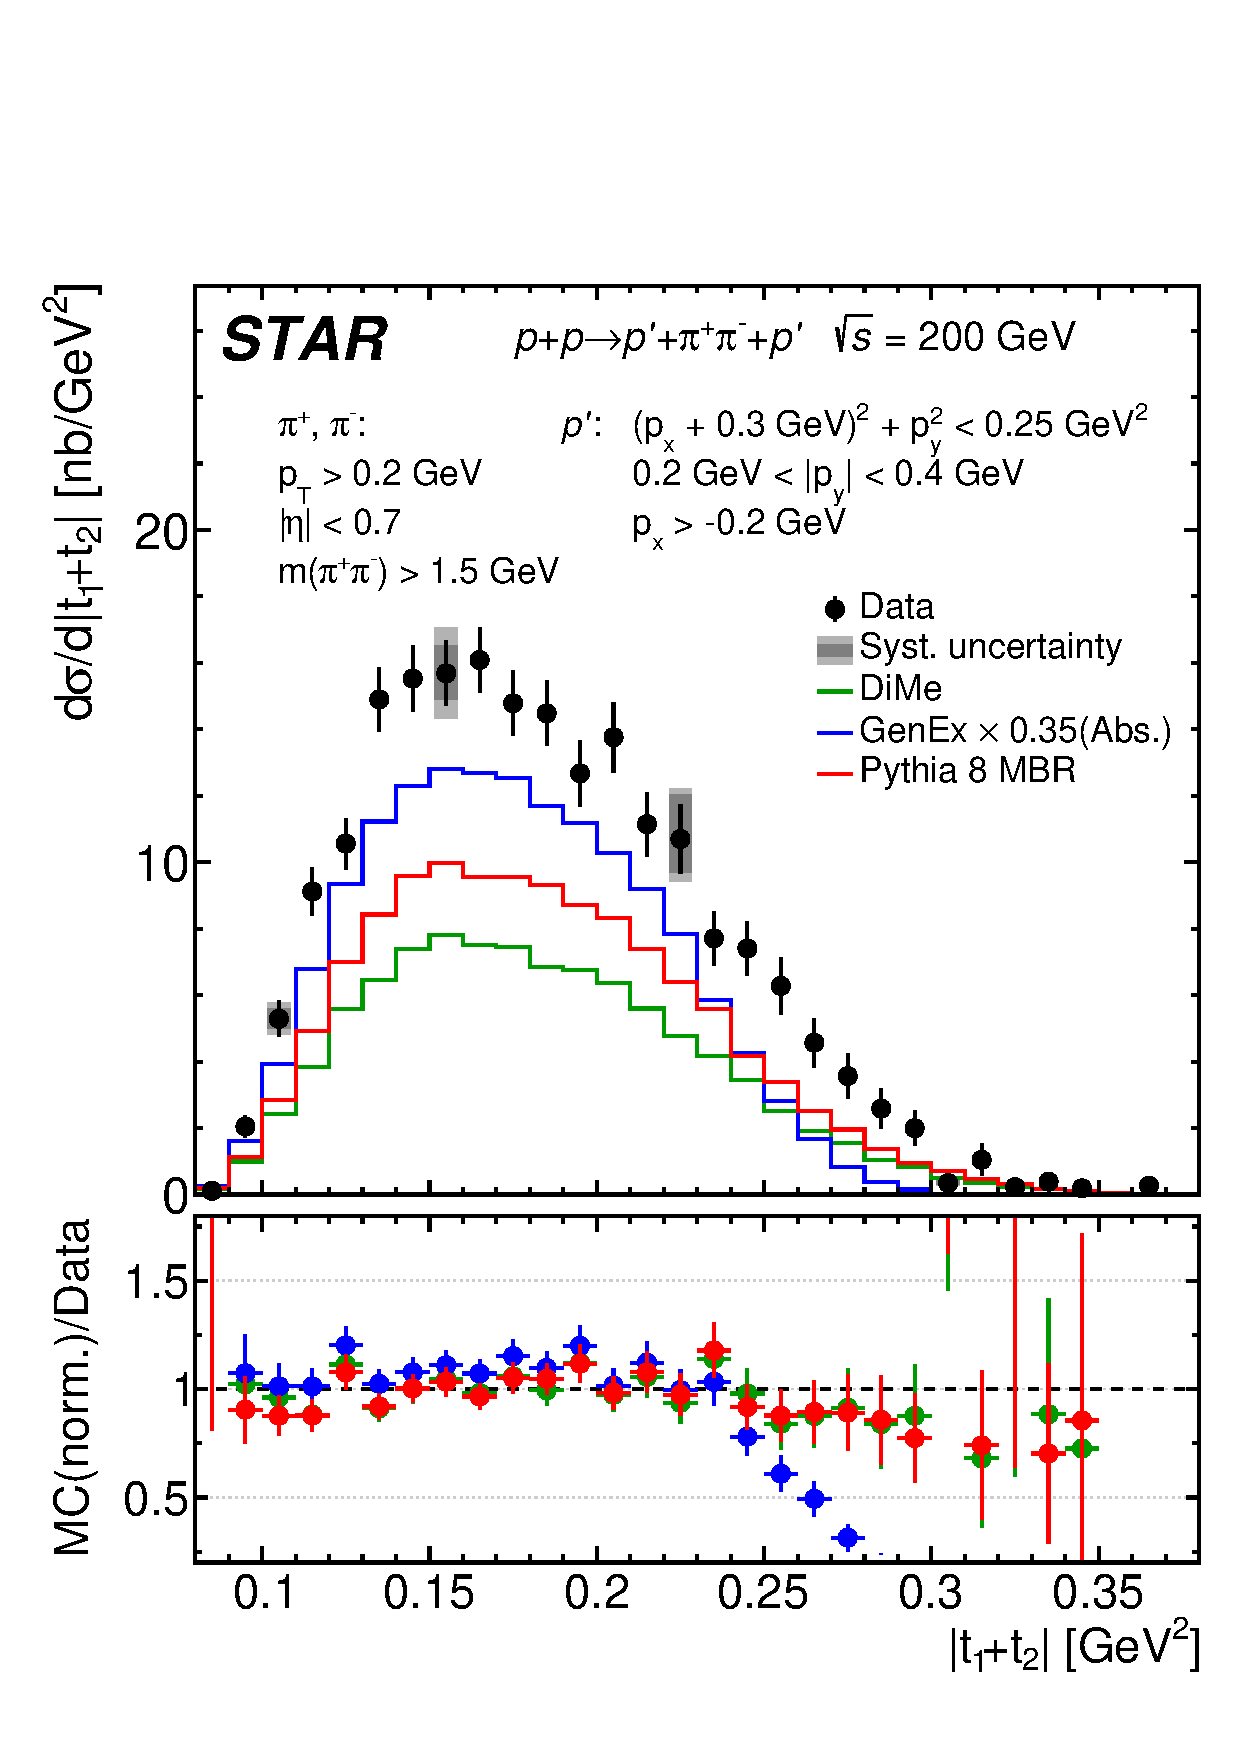
\includegraphics[width=.31\textwidth,page=1]{graphics/physicsResults/Ratio_FinalResult_MandelstamTSum_pion_MassBin_3.pdf}
%
\caption{Differential cross sections for CEP of $\pi^+\pi^-$ pairs as a function of the rapidity of the pair (left column) difference of azimuthal angles of the forward scattered protons (middle column) and of the sum of the squares of the four-momenta losses in the proton vertices (right column) measured in the fiducial region explained on the plots, separately for three ranges of the $\pi^+\pi^-$ pair invariant mass: $m<1$ GeV (top), $1<m<1.5$ GeV (middle) and $m>1.5$ GeV (bottom). Data are shown as solid points with error bars representing the statistical uncertainties. The typical systematic uncertainties are shown as gray boxes for only few data points as they are almost fully correlated between neighboring bins. Predictions from MC models GenEx, DiMe and MBR are shown as histograms. In the lower panels the ratios of the MC predictions scaled to data and the data are shown.}
\label{results_4}
\end{figure}
%
%\FloatBarrier
%
\begin{figure}[h]
\centering
\hspace*{5pt}
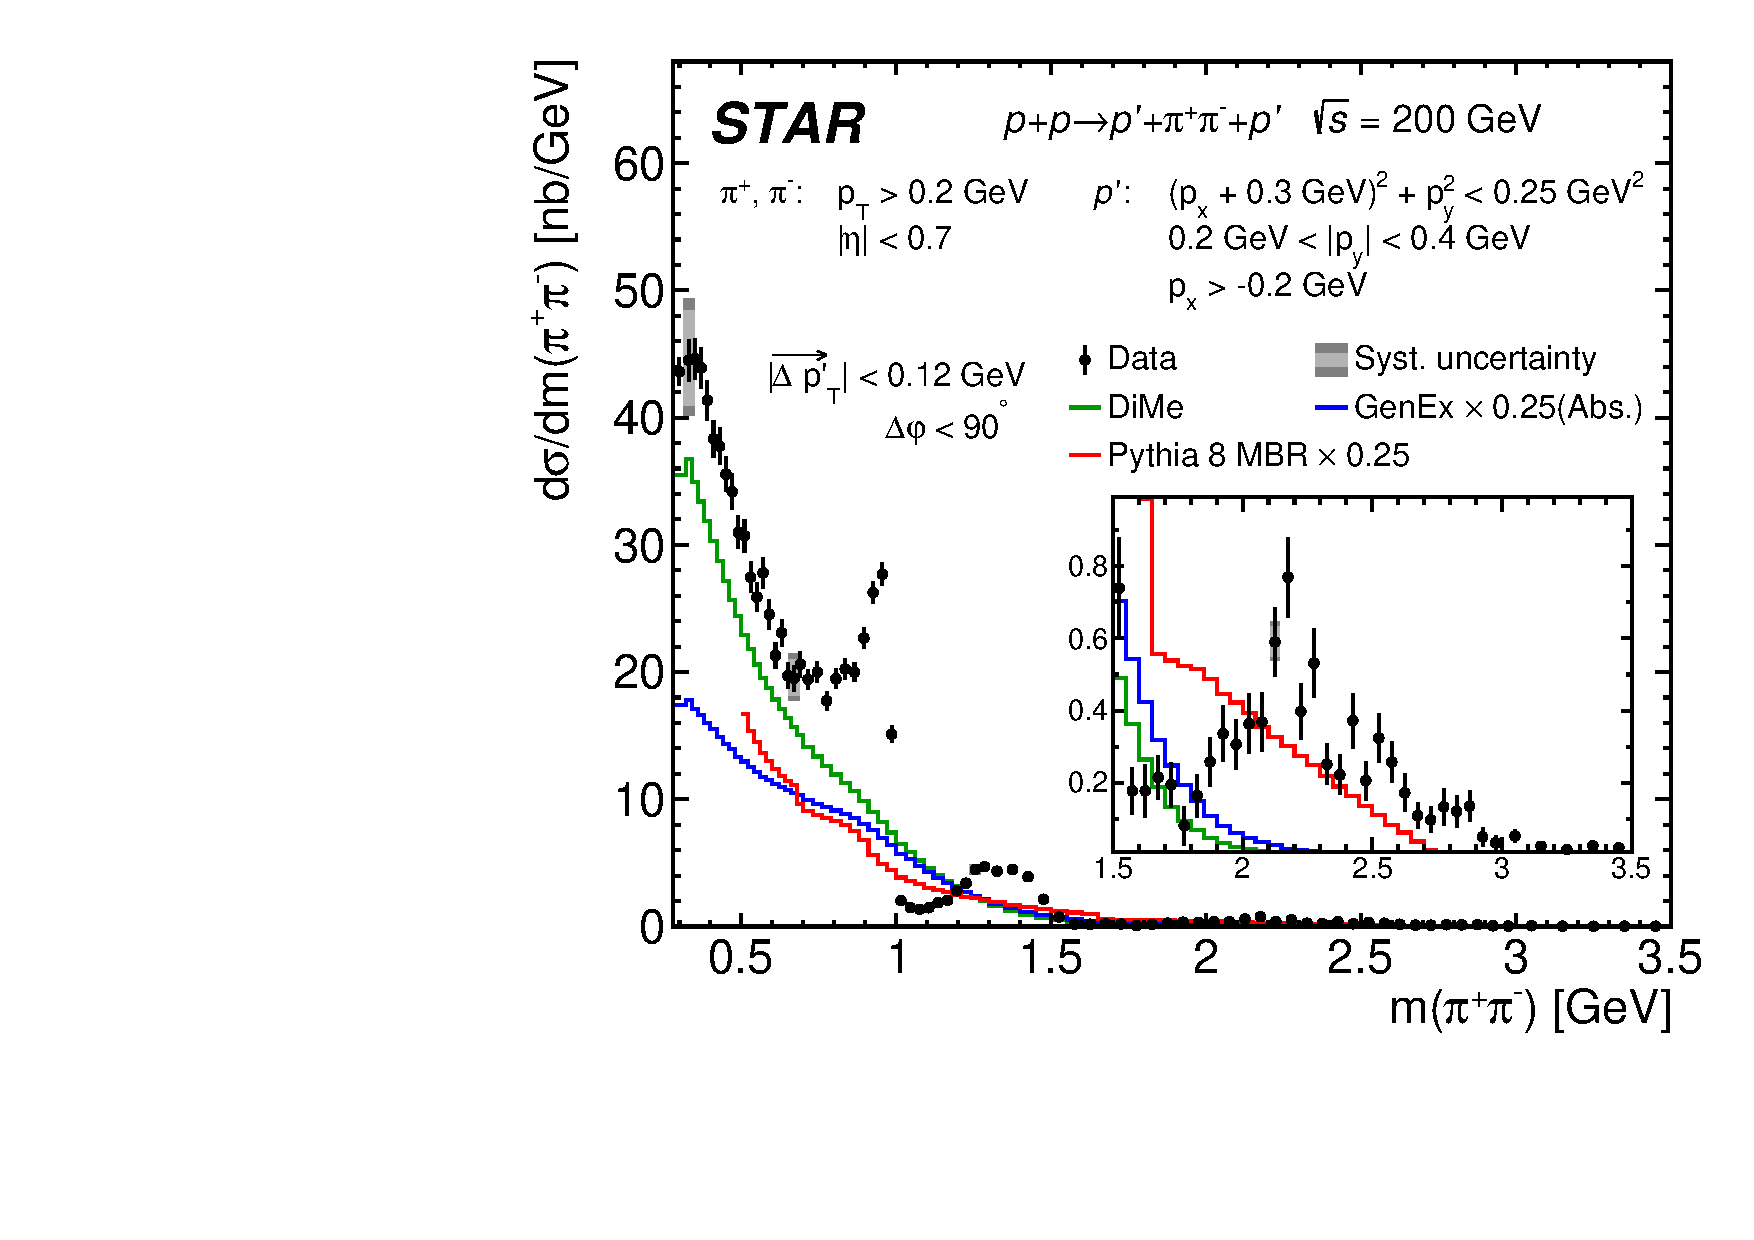
\includegraphics[width=.46\textwidth,page=1]{graphics/physicsResults/FinalResult_InvMass_pion_SmallDpt_DeltaPhiLessThan90.pdf}
\hfill
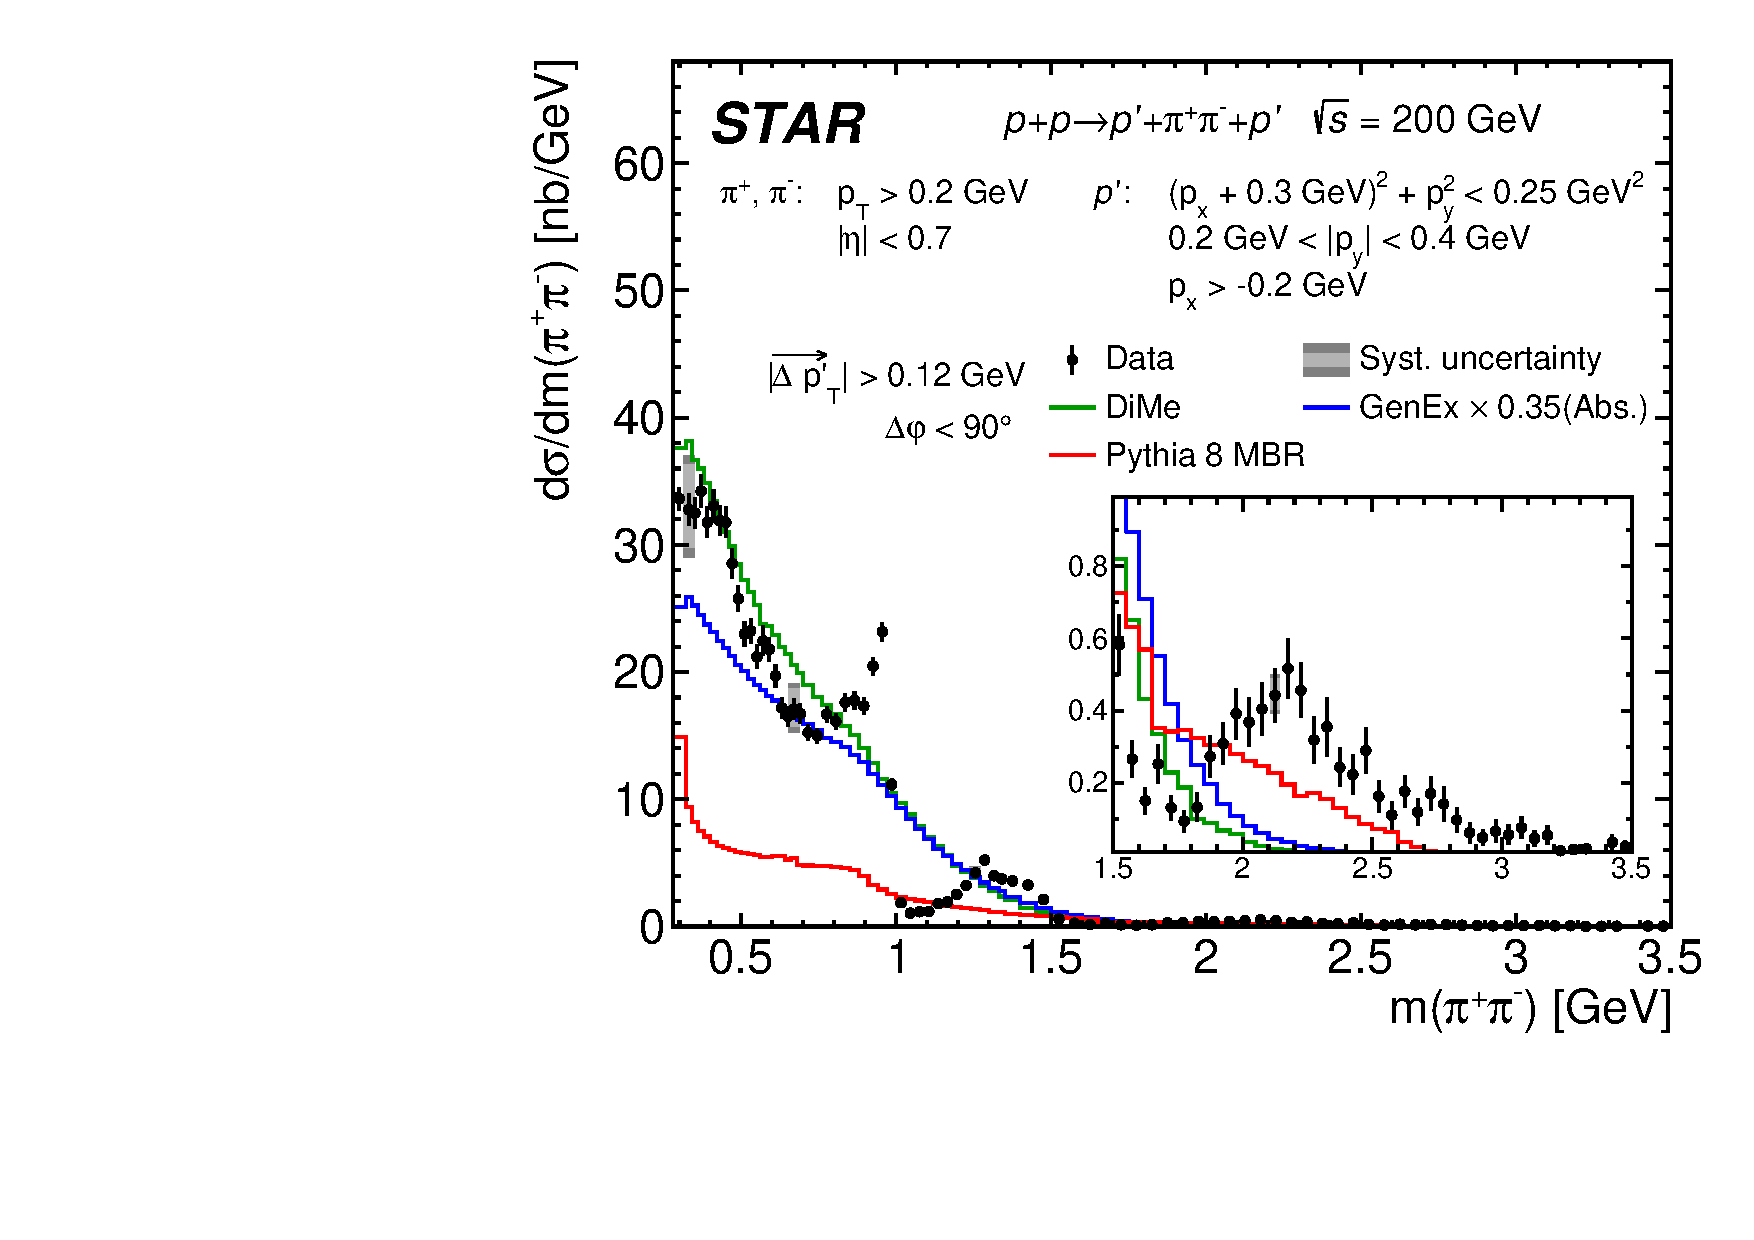
\includegraphics[width=.46\textwidth,page=1]{graphics/physicsResults/FinalResult_InvMass_pion_LargeDpt_DeltaPhiLessThan90.pdf}
\hspace*{5pt}
%
\caption{Differential cross sections $d\sigma/dm(\pi^+\pi^-)$ for CEP of $\pi^+\pi^-$ pairs in two $|\vec{p}_{1,T}^{\,\prime}-\vec{p}_{2,T}^{\,\prime}|$ regions: $|\vec{p}_{1,T}^{\,\prime}-\vec{p}_{2,T}^{\,\prime}|<0.12$ GeV (left) and $|\vec{p}_{1,T}^{\,\prime}-\vec{p}_{2,T}^{\,\prime}|>0.12$ GeV (right)  in the fiducial region and $\Delta\phi<90$ degree. There is no difference for two $|\vec{p}_{1,T}^{\,\prime}-\vec{p}_{2,T}^{\,\prime}|$ regions. Data are shown as solid points with error bars representing the statistical uncertainties. The typical systematic uncertainties are shown as gray boxes for only few data points as they are almost fully correlated between neighboring bins. Predictions from MC models GenEx, DiMe and MBR are shown as histograms.}
\label{results_5}
\end{figure}


% We have also studied angular distributions of the charged particles produced in the final state. This can be done in various reference frames. However, for an easy comparison with theoretical predictions we use here the Collins-Soper \cite{cs_frame} reference frame also used e.g. in Ref.~\cite{lebiedowicz_3}. Collins-Soper frame is the centre-of-mass frame of the charged particles pair with the $z$-axis making equal angles with the beam protons momenta which in addition define the new $x-z$ plane. It can be reached from the laboratory frame (proton-proton c.m.s.) in two steps. First, boost along the $z$-axis to an intermediate frame in which the pair longitudinal momentum is equal to zero. In this frame the beam protons momenta remain parallel to the $z$-axis and the transverse momentum of the pair remains unchanged. Second, boost in the direction of the transverse momentum of the pair, to get to the pair c.m.s. frame.
%
\begin{figure}[h]
\centering
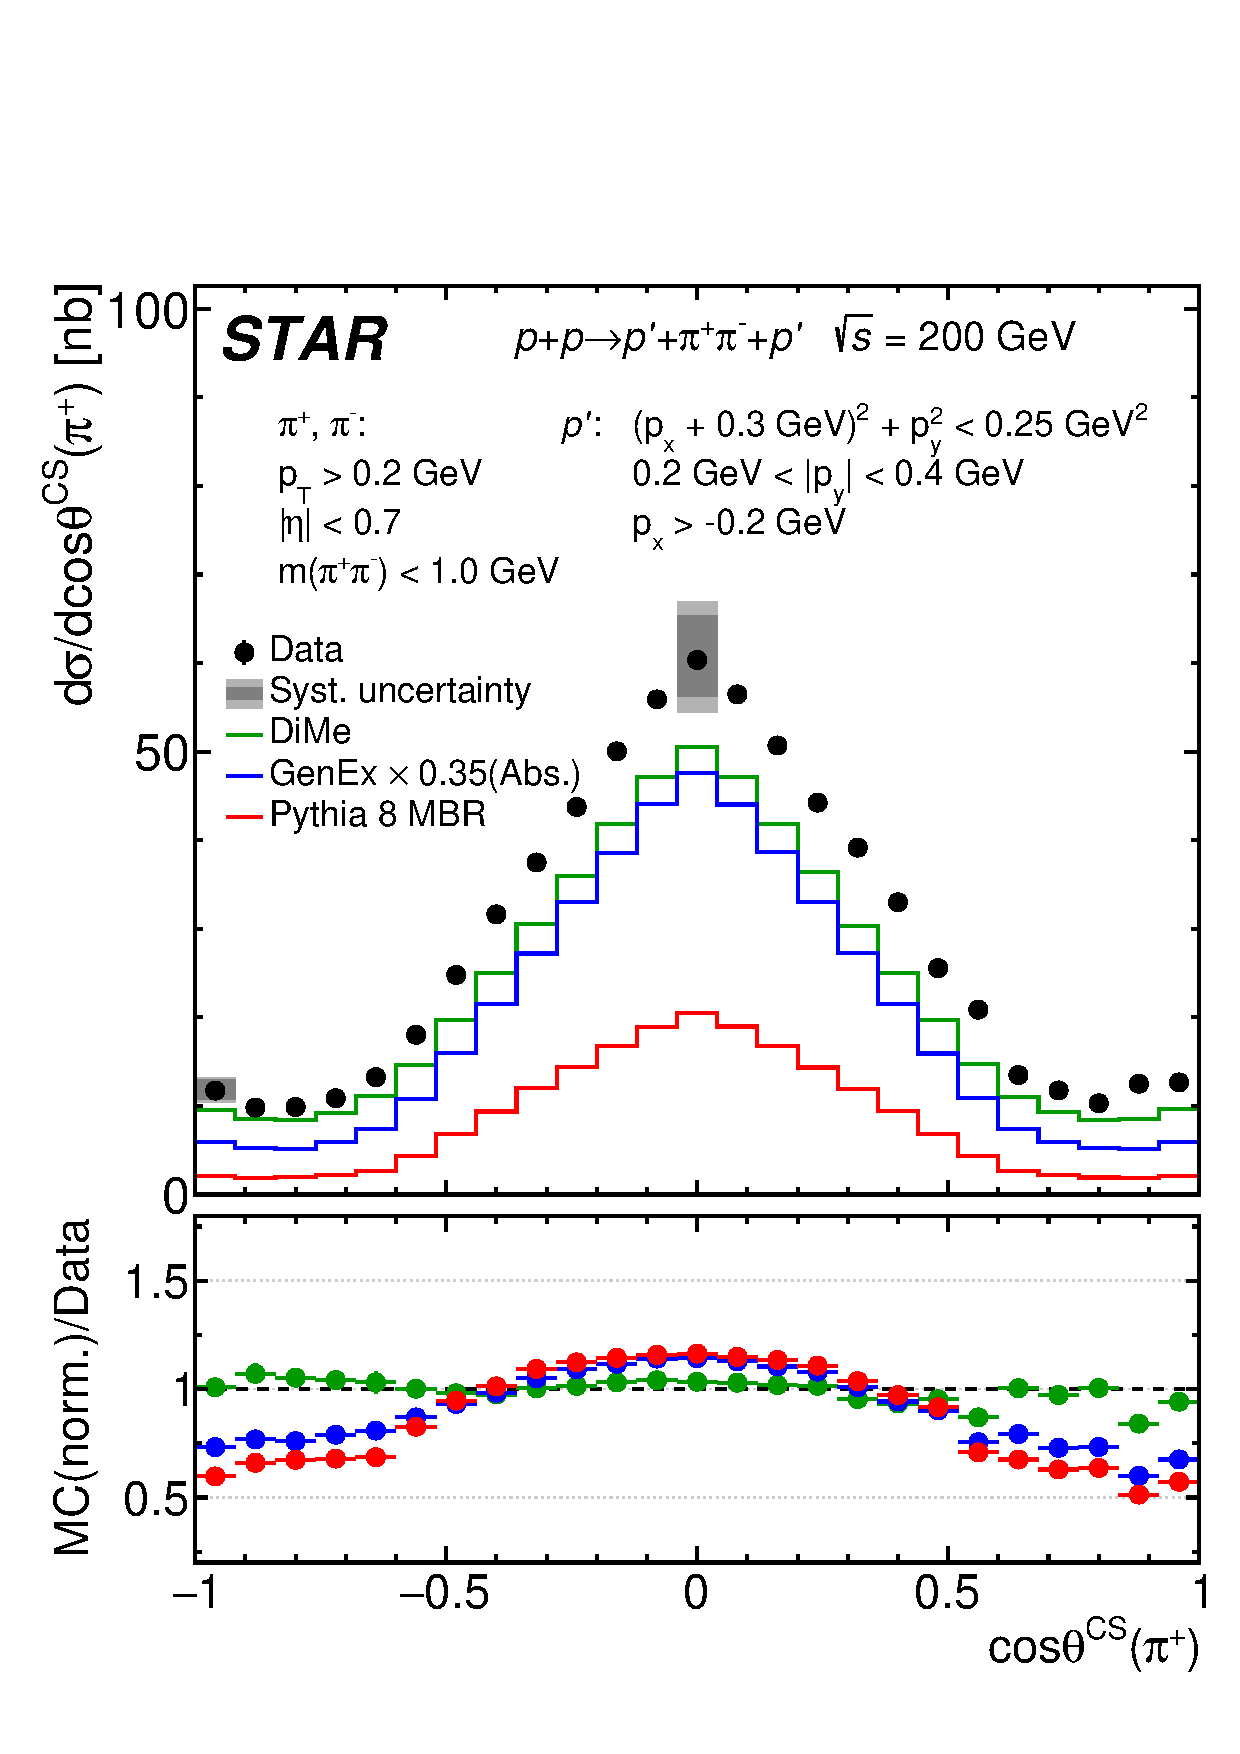
\includegraphics[width=.31\textwidth,page=1]{graphics/physicsResults/Ratio_FinalResult_CosThetaCS_pion_MassBin_1.pdf}
\hfill
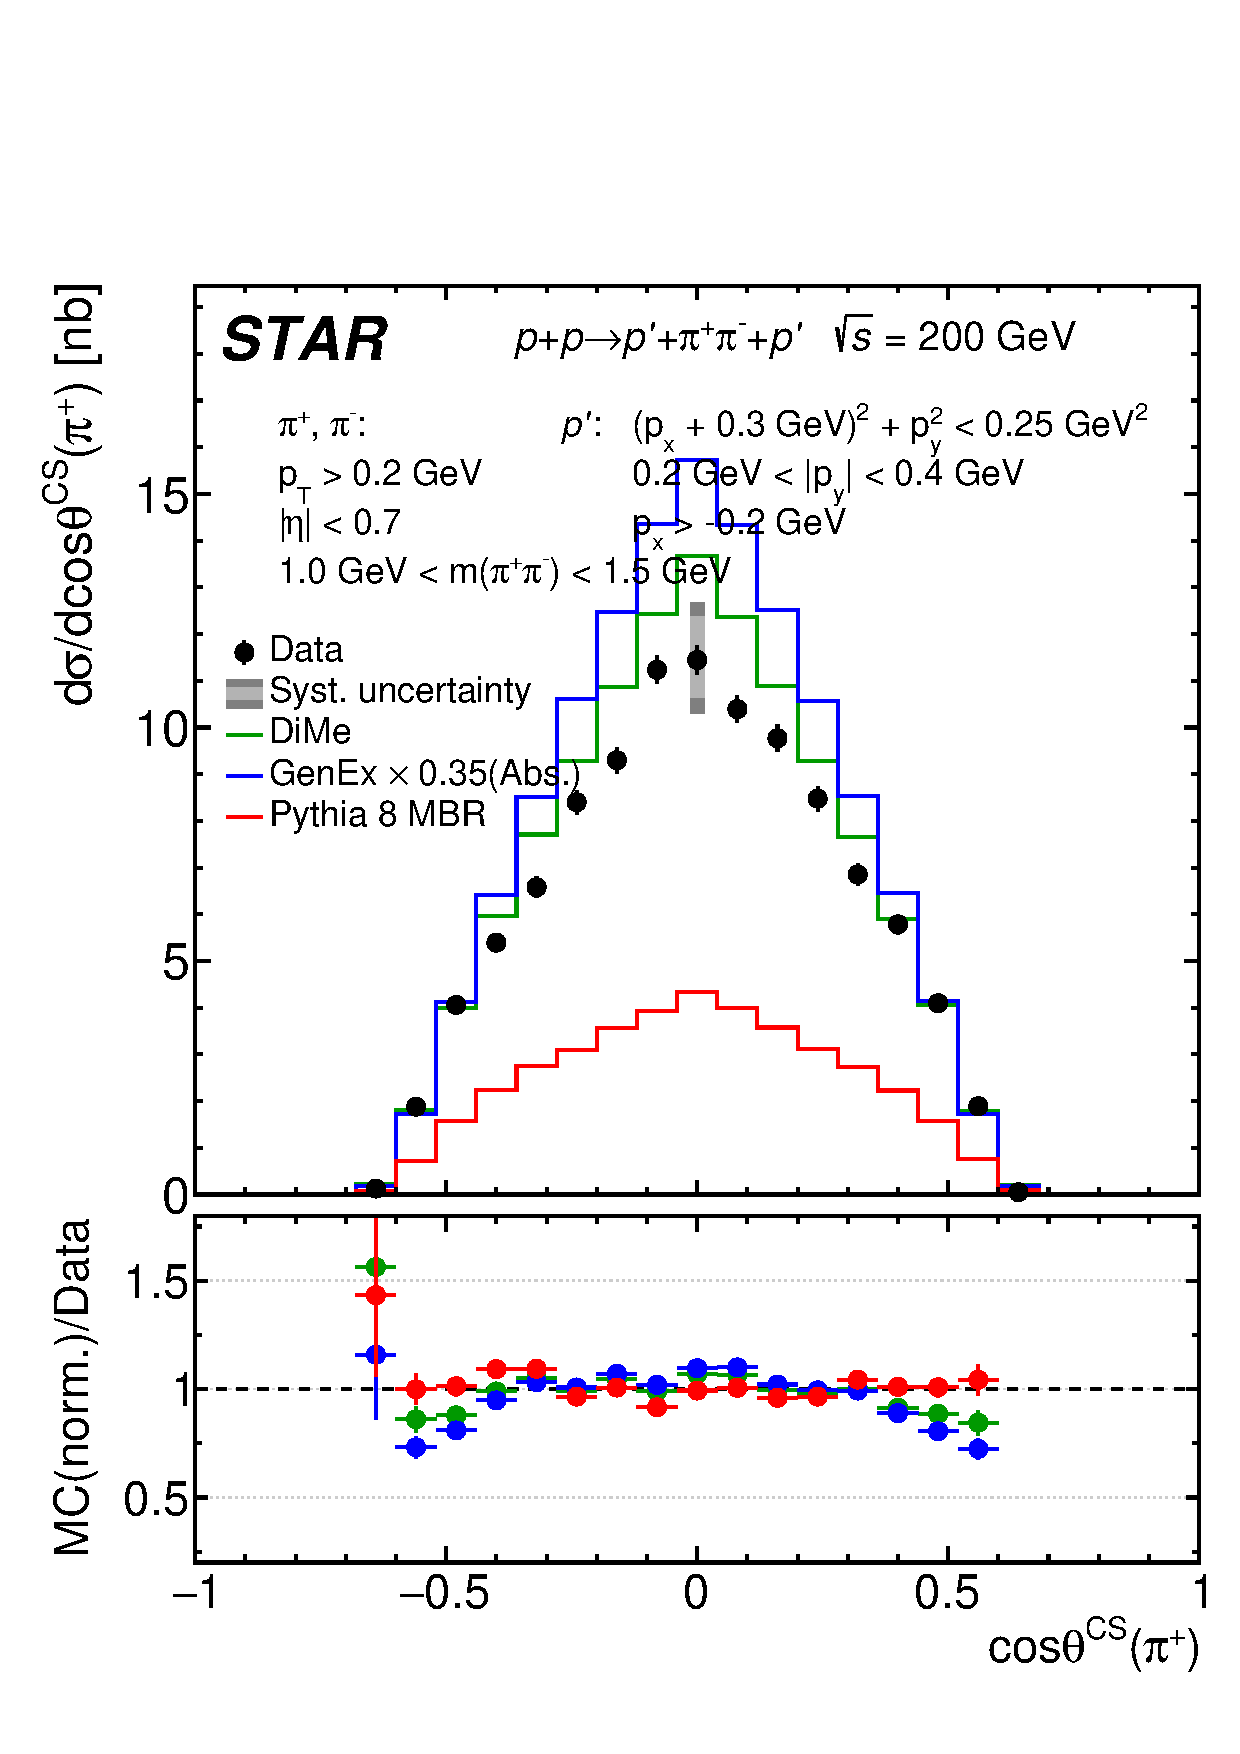
\includegraphics[width=.31\textwidth,page=1]{graphics/physicsResults/Ratio_FinalResult_CosThetaCS_pion_MassBin_2.pdf}
\hfill
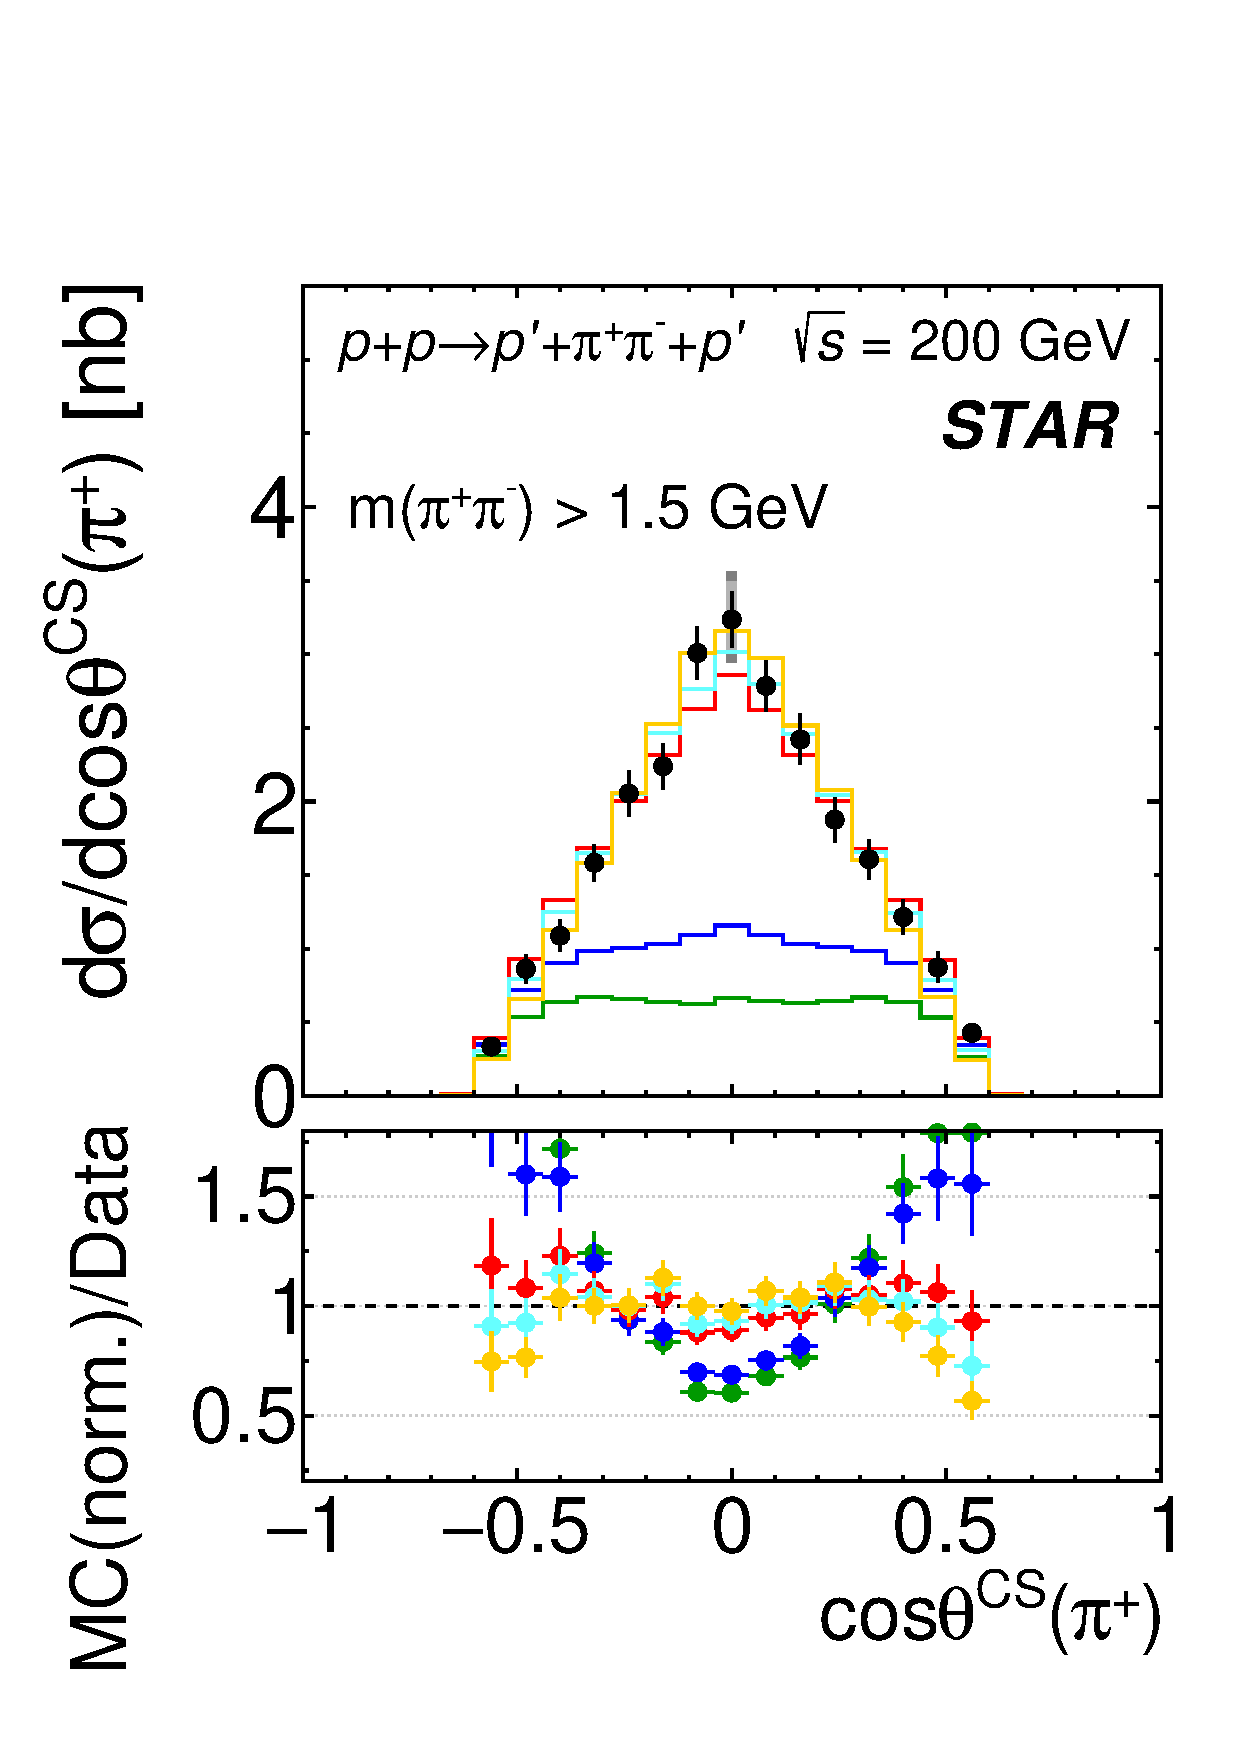
\includegraphics[width=.31\textwidth,page=1]{graphics/physicsResults/Ratio_FinalResult_CosThetaCS_pion_MassBin_3.pdf}
\newline
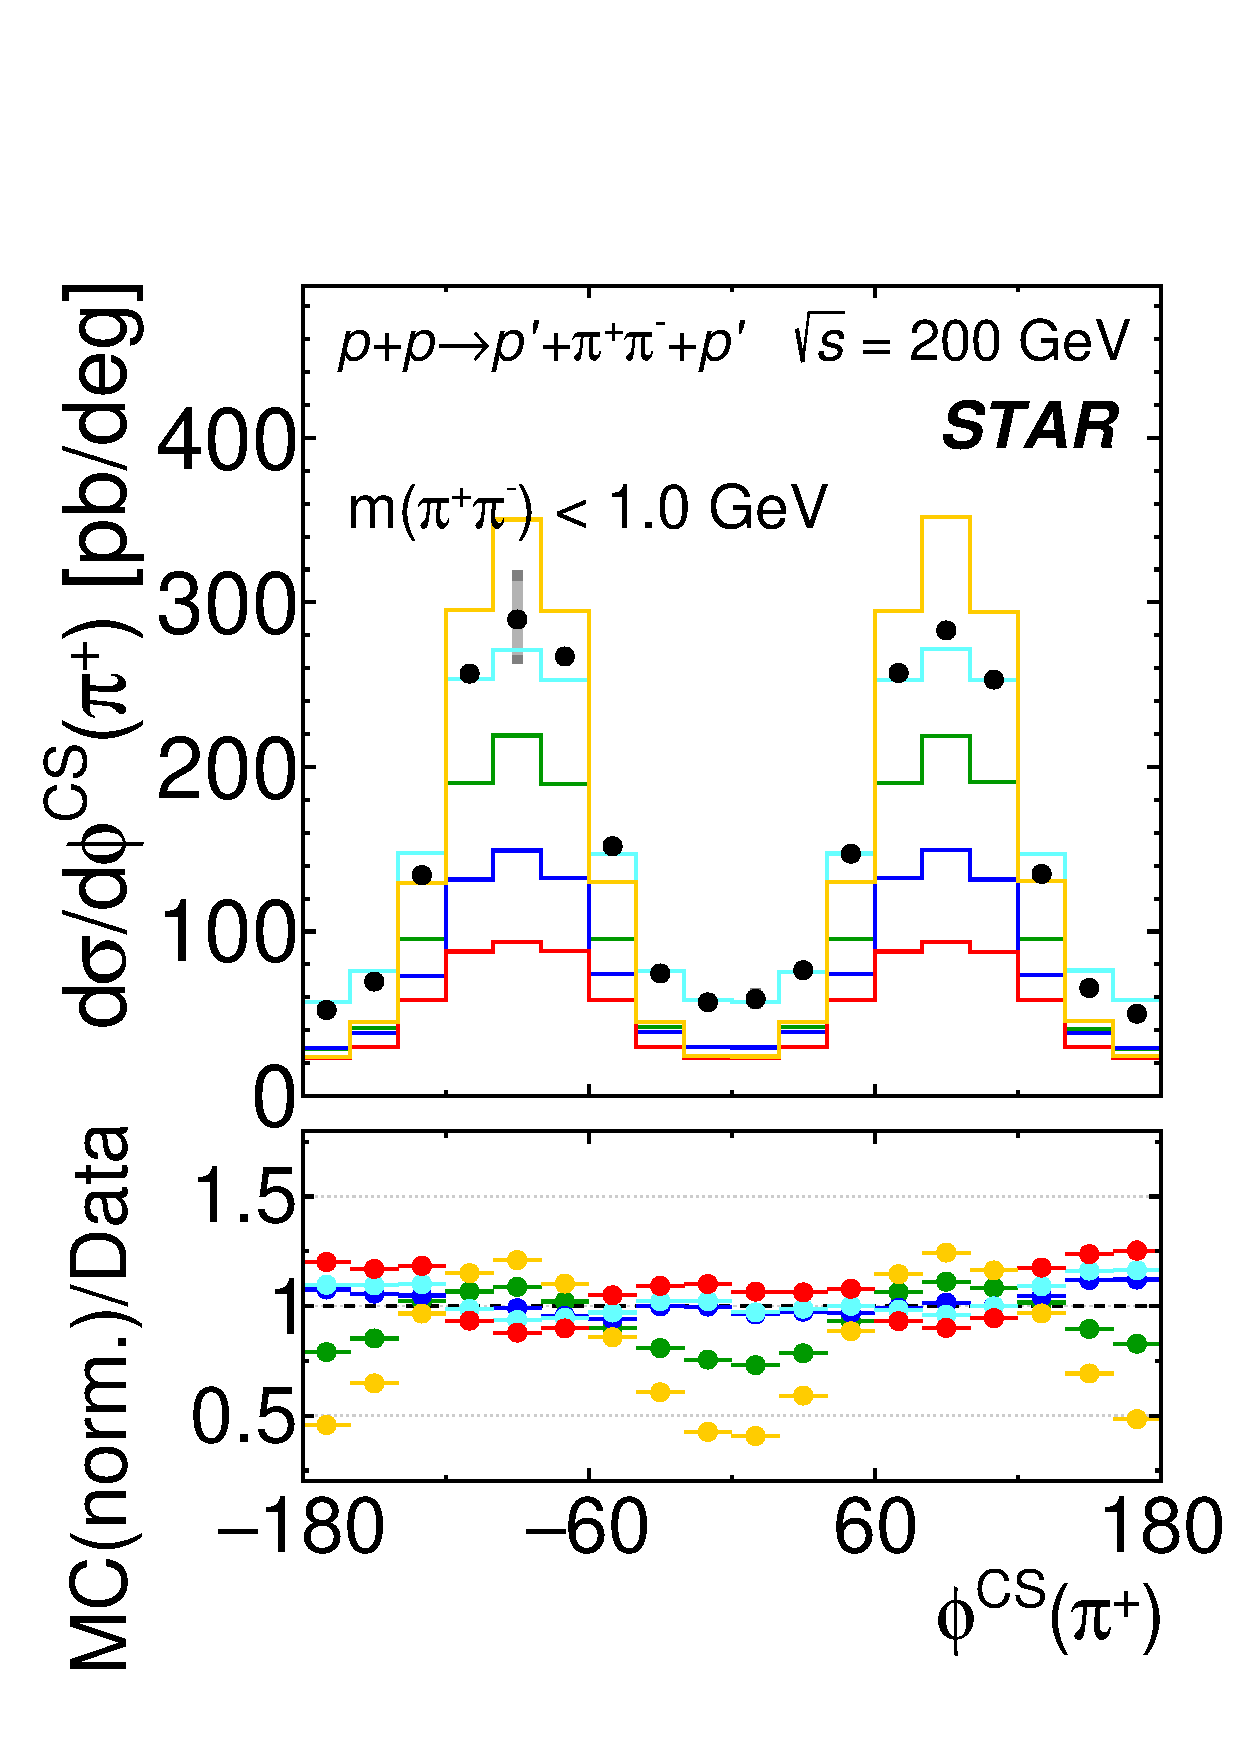
\includegraphics[width=.31\textwidth,page=1]{graphics/physicsResults/Ratio_FinalResult_PhiCS_pion_MassBin_1.pdf}
\hfill
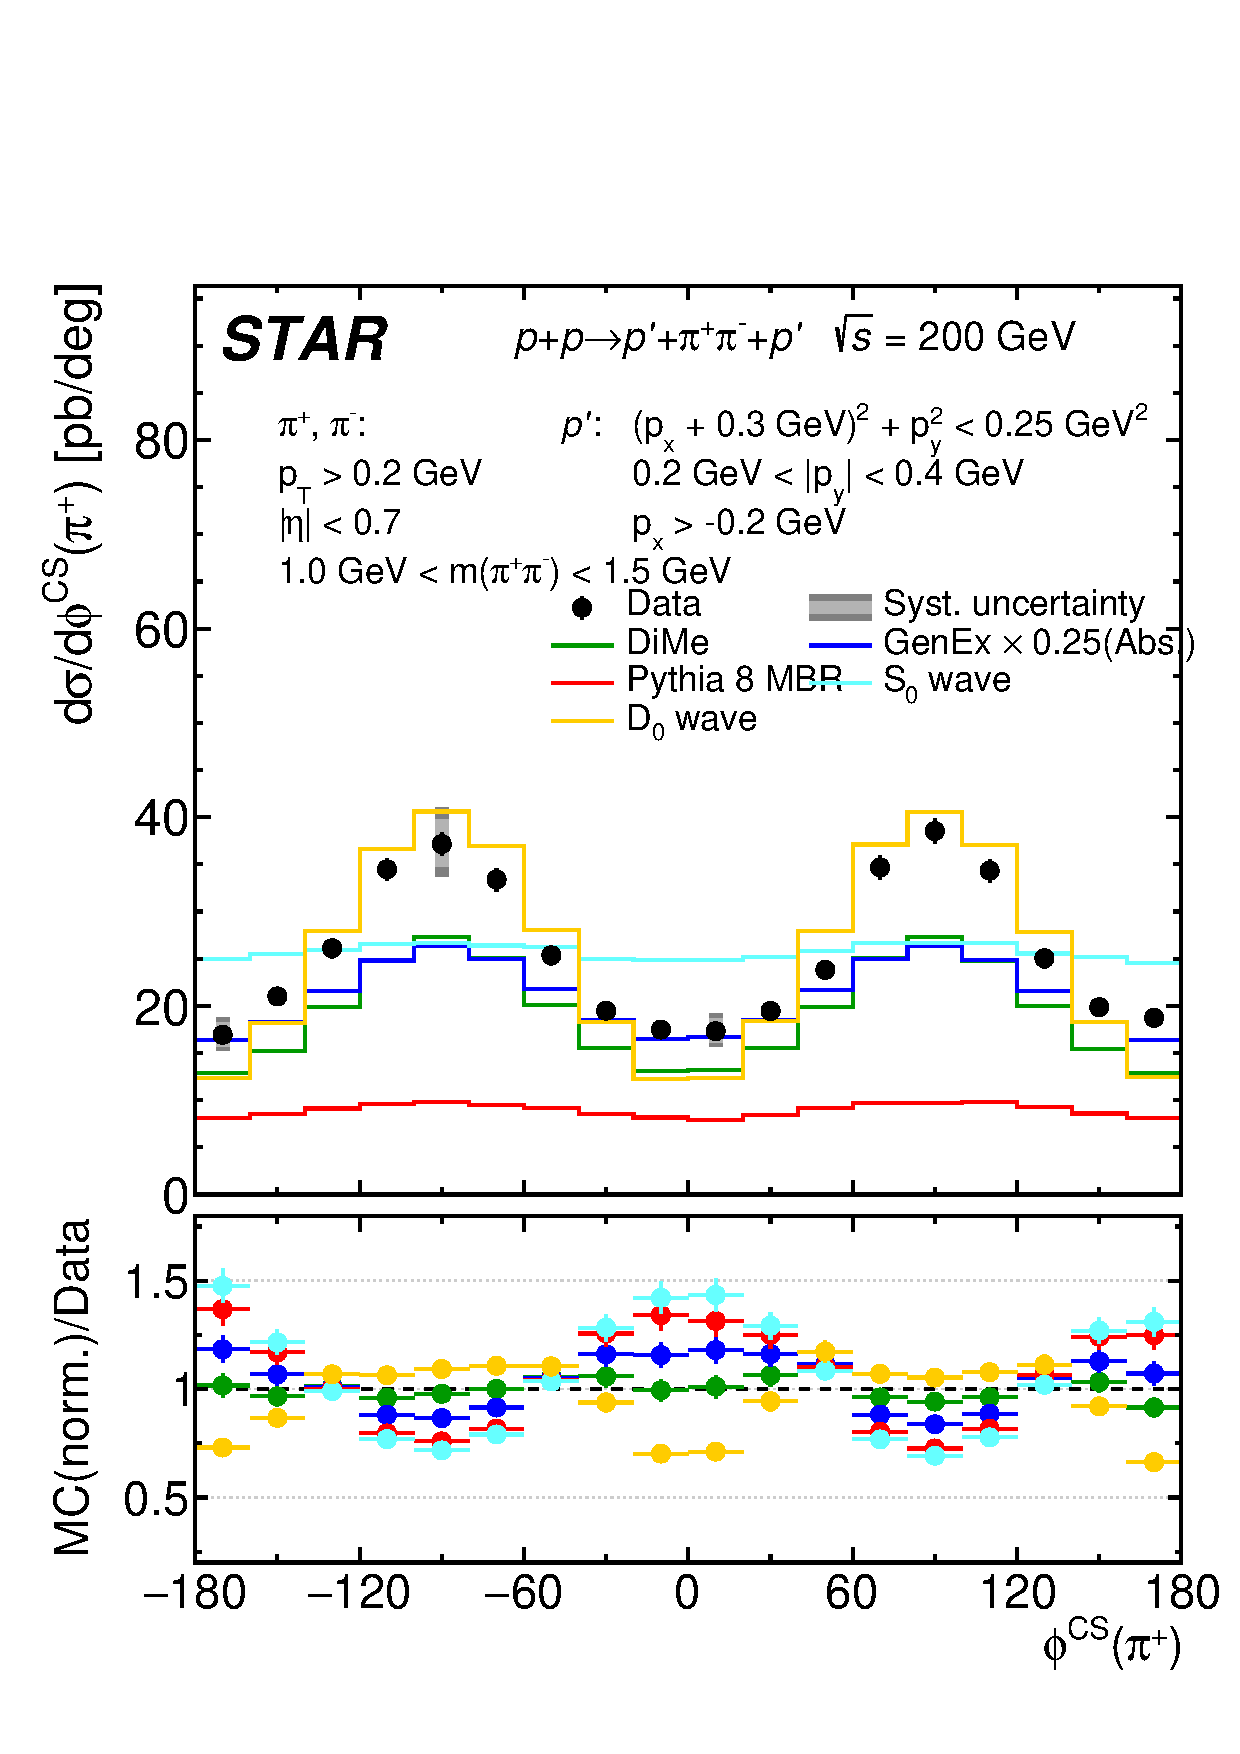
\includegraphics[width=.31\textwidth,page=1]{graphics/physicsResults/Ratio_FinalResult_PhiCS_pion_MassBin_2.pdf}
\hfill
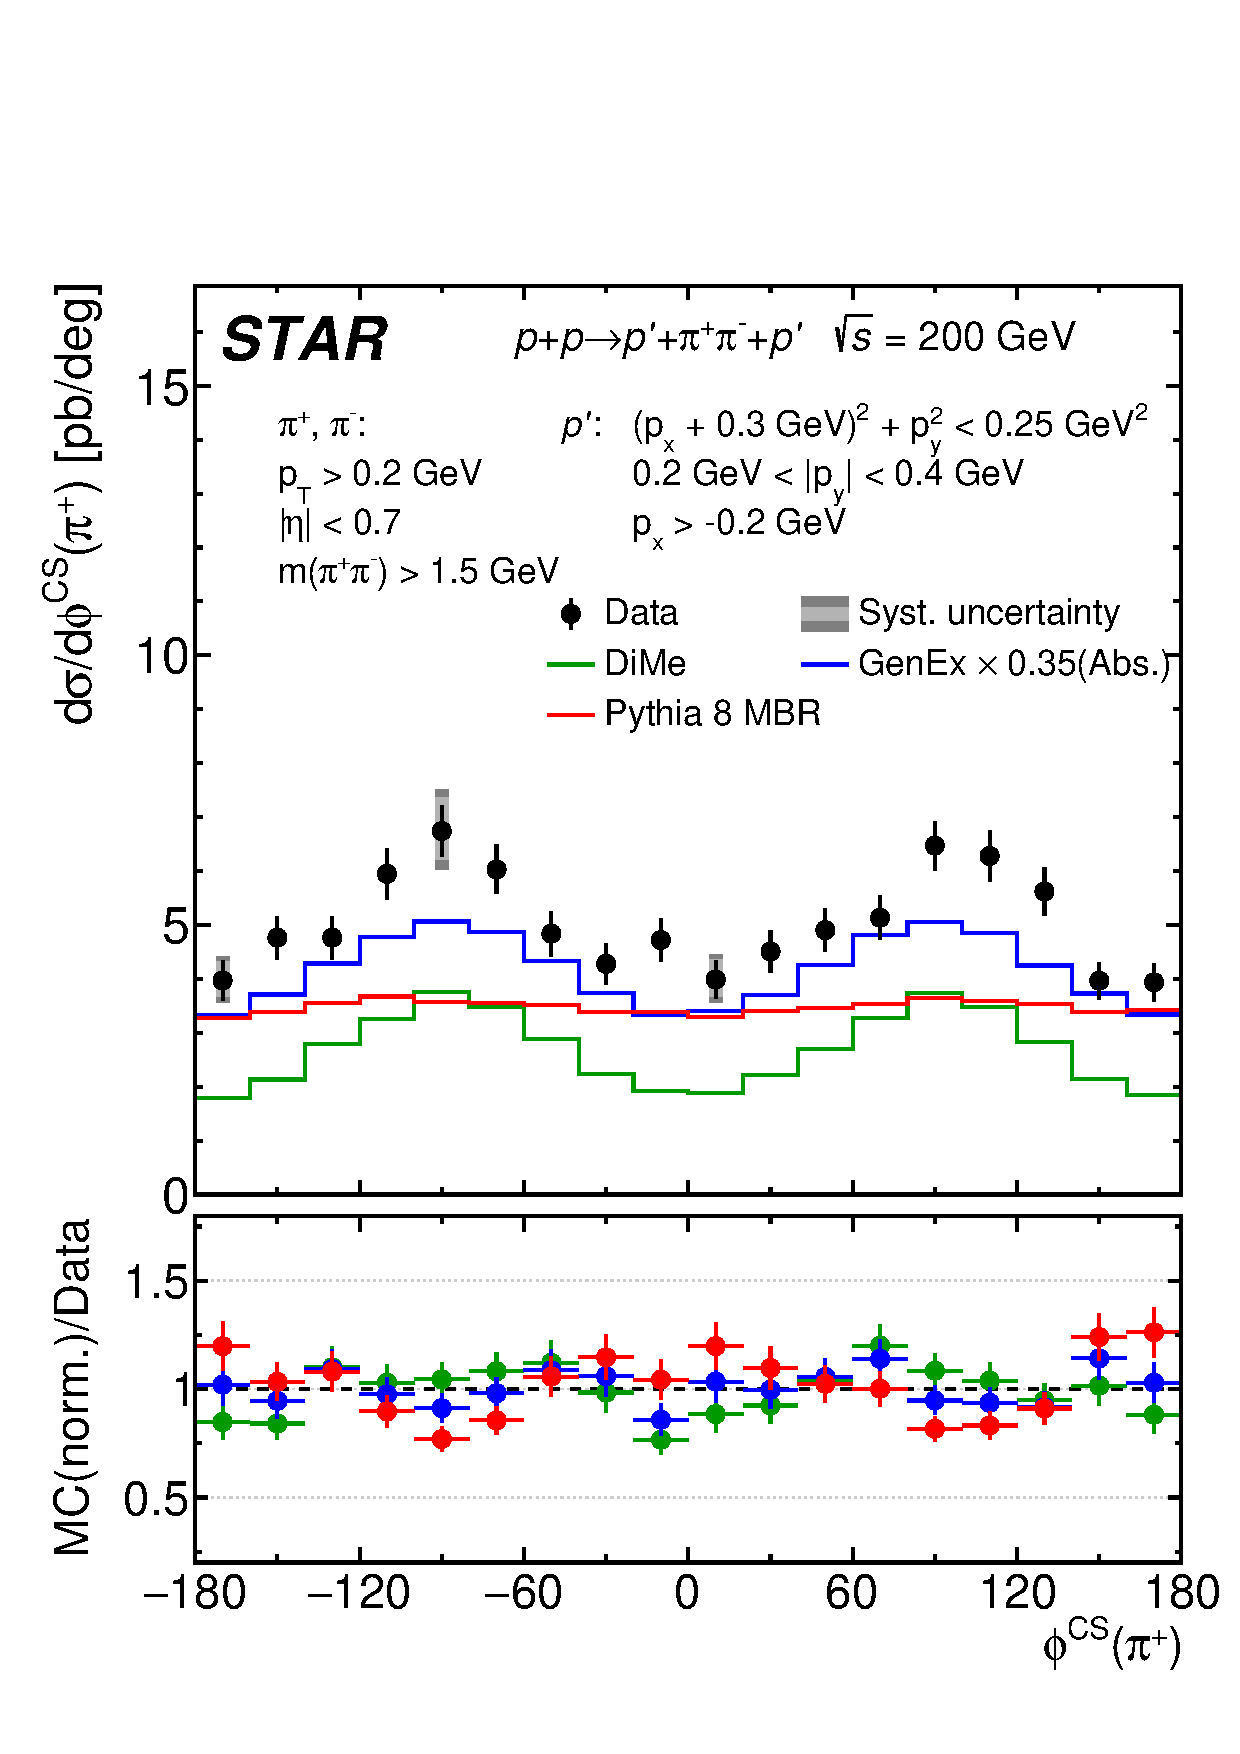
\includegraphics[width=.31\textwidth,page=1]{graphics/physicsResults/Ratio_FinalResult_PhiCS_pion_MassBin_3.pdf}
%
\caption{Differential cross sections for CEP of $\pi^+\pi^-$ pairs as a function of $\cos{\theta^\mathrm{CS}}$ (top) and of $\phi^\mathrm{CS}$ (bottom)  measured in the fiducial region explained on the plots, separately for three ranges of the $\pi^+\pi^-$ pair invariant mass: $m<1$ GeV (left column), $1<m<1.5$ GeV (middle column) and $m>1.5$ GeV (right column). Data are shown as solid points with error bars representing the statistical uncertainties. The typical systematic uncertainties are shown as gray boxes for only few data points as they are almost fully correlated between neighboring bins. Predictions from MC models GenEx, DiMe and MBR are shown as histograms. In the lower panels the ratios of the MC predictions scaled to data and the data are shown.}
\label{results_7}
\end{figure}


\section{Invariant mass spectrum modelling}

Invariant mass distributions in the fiducial region of the measurement can not be directly used to extract yields of possible resonances without extrapolation to the full kinematic region of the central pions pair, given by $p_\mathrm{T}\rightarrow 0$ and $|\eta|\rightarrow\infty$  (full solid angle in the central system rest frame). Extrapolation to unmeasured region is always model dependent. In this section we present cross-section corrected to the full phase-space using the angular flat approximation which leaves scalar decays uniform over the solid angle in the rest frame of the central system. To limit the corrections, the measurement is restricted to $|y(\pi^+\pi^-)|<0.4$ which keeps scalar decays uniform, by Lorentz invariance. In the correction calculation factorisation of the central system and forward protons phase space is assumed. For the forward protons phase space a uniform distributions of the azimuthal angles are assumed while polar angles are generated according to exponential $t$ distribution with $t$-slope of 6~GeV$^{-2}$. 
%The measurement is extrapolated from fiducial region given by Eq.~\eqref{fp_fiducial} to the Lorentz invariant $0.05 \leq -t_1 , -t_2 \leq 0.16$ GeV$^2$ region.
The measurement is extrapolated from the part of the fiducial region given by Eq.~\eqref{eq:RpFiducial} covering $0.05 \leq -t_1 , -t_2 \leq 0.16$ GeV$^2$ to such defined Lorentz invariant $t$ interval and full azimuthal angle of forward protons.
The measurement is further restricted to two regions of $\Delta\varphi<45^\circ$ and $\Delta\varphi>135^\circ$ which reduces size of acceptance corrections and related systematic uncertainties.

We make an attempt to fit extrapolated differential cross-section with a simplified model of the $\pi^{+}\pi^{-}$ invariant mass spectrum. In this model we assume contributions from the direct pair production and three resonances in the mass range of $0.6-1.7$ GeV: $f_0(980)$, $f_2(1270)$ and $f_0(1500)$. The total amplitude for the exclusive $\pi^{+}\pi^{-}$ production is then given by:
%
\begin{equation}
\label{eq:amplitude}
\begin{aligned}
A(m) = & \;A_{\textrm{cont}}\times f_{\textrm{cont}(m)}+ \\
        & \;A_{\textrm{f}_0(980)} \times \mathcal{R}_{\textrm{F}}\left(m;M_{f_0(980)},\Gamma_{f_0(980)}\right)+ \\
        & \;A_{\textrm{f}_2(1270)} \times \mathcal{R}_{\textrm{BW}}\left(m;M_{f_2(1270)},\Gamma_{f_2(1270)}\right) +\\
        & \;A_{\textrm{f}_0(1500)} \times \mathcal{R}_{\textrm{BW}}\left(m;M_{f_0(1500)},\Gamma_{f_0(1500)}\right),\\
\end{aligned}
\end{equation}
%
thus all states are added coherently (interfere with each other). The amplitude for continuum production is chosen to be real while multiplicative amplitude factors for resonances are allowed to be complex:
\begin{equation}A_{\textrm{cont}}\in\mathbb{R},~~~A_{\textrm{f}_0(980)},A_{\textrm{f}_2(1270)},A_{\textrm{f}_0(1500)}\in\mathbb{C}~~~~\rightarrow~~~~A_{\textrm{f}}=|A_{\textrm{f}}|e^{i\phi_{\textrm{f}}}.\end{equation}
%
The shape of the continuum amplitude is assumed to have the form
\begin{equation}f_{\textrm{cont}}(m) = \sqrt{\frac{q}{m}}\times e^{-\frac{B}{2}\cdot m}\end{equation}
with the break-up momentum $q$ equal to
\begin{equation}\label{eq:breakupMom}
q(m) = \frac{1}{2}\sqrt{m^{2}-4m_{\pi}^{2}}.
\end{equation}
For $f_2(1270)$ and $f_0(1500)$ resonances we use relativistic Breit-Wigner form of the production amplitude with mass-dependent width:
\begin{equation}\label{eq:BW}\mathcal{R}_{\textrm{BW}}(m;M,\Gamma_{0}) = \frac{M\sqrt{\Gamma_{0}}\sqrt{\Gamma(m)}}{M^{2}-m^{2}-i M\Gamma(m)},~~\Gamma(m) = \Gamma_{0}\frac{q}{m}\frac{M}{q_{0}}\left(\frac{B_{J}(q^{2}R^{2})}{B_{J}(q_{0}^{2}R^{2})}\right)^{2}.\end{equation}
The centrifugal effects in Eq.~\eqref{eq:BW} are accounted through the Blatt-Weisskopf barrier factors $B_{J}$~\cite{BarrierFactors} with the empirical interaction radius $R$ set to 1~fm and $q_{0} = q(M)$. Naturally $J=2$ and $J=0$ is used for $f_2(1270)$ and $f_0(1500)$, respectively.

Meson $f_0(980)$ requires different treatment due to large branching ratio to $K\bar{K}$ channel which opens in the vicinity of the mass peak. This changes the resonance shape and is accounted for in the parametrisation of the amplitude via the Flatt\'e formula~\cite{Flatte}:
\begin{equation}\label{eq:Flatte}\mathcal{R}_{\textrm{F}}(m;M,\Gamma_{0}) = \frac{M\sqrt{\Gamma_{0}}\sqrt{\Gamma_{\pi}(m)}}{M^{2}-m^{2}-i M\left(\Gamma_{\pi}(m)+\Gamma_{K}(m)\right)}\end{equation}
%
with the partial width $\Gamma_{j}$ ($j=\pi, K$) described by the product of the coupling parameter $g_{j}$ and the break-up momentum $q$ (Eq.~\eqref{eq:breakupMom}) for particle $j$:
\begin{equation}
    \Gamma_{j}(m) = g_{j}q_{j}(m) = \frac{g_{j}}{2}\sqrt{m^{2}-4m_{j}^{2}}.
\end{equation} and the partial width in $\pi^{+}\pi^{-}$ channel at the resonance mass equal to
\begin{equation}
    \Gamma_{0} = g_{\pi}q_{\pi}(M).
\end{equation}
In the fit the ratio $g_{K}/g_{\pi}$ is fixed to 4.21, the value well constrained experimentally through the measurement of $J/\psi$ decay into $\phi$ and $\pi^{+}\pi^{-}$/$K^{+}K^{-}$~\cite{BES_JPsi}.
%

Squared amplitude from Eq.~\eqref{eq:amplitude}, $|A|^{2}$, is convoluted for the purpose of the fit with the normal distribution $\mathcal{N}(m; \sigma_{\text{res}})$ representing finite resolution of reconstructed invariant mass of the pion pair. The resolution parameter $\sigma_{\text{res}}$ is provided to the fitting algorithm; it is set to grow linearly with increasing invariant mass according to MC simulation of the STAR TPC detector. The $m(\pi^{+}\pi^{-})$ resolution at the lower and upper limit of the fit range is equal to 4~MeV and 13~MeV, respectively. The final form of function fitted to extrapolated $d\sigma/dm(\pi^{+}\pi^{-})$ is given by
\begin{equation}
    \mathcal{F}(m) = \int\limits_{m-3.5\cdot\sigma_{\text{res}}(m)}^{m+3.5\cdot\sigma_{\text{res}}(m)}dm'\mathcal{N}\left(m'-m; \sigma_{\text{res}}(m)\right)|A(m')|^{2}.
\end{equation}

The fitting is performed using Minuit2 toolkit~\cite{Minuit2} within the ROOT analysis software~\cite{ROOT}. The standard-defined $\chi^{2}$ is minimized simultaneously in two $\Delta\varphi$ ranges with the masses and widths of both $f_0$'s forced to be equal, while phases and absolute values of $f_2$ and $f_0$'s amplitudes left independent in the two $\Delta\varphi$ subsets. The mass and width of $f_2(1270)$ resonance is fixed to the well known Particle Data Group values~\cite{pdg}.
%

Systematic uncertainties of the model parameters are estimated through the independent fits to extrapolated $d\sigma/dm(\pi^{+}\pi^{-})$ with applied each of the systematic variations described in Sec.~\ref{sec:systematics}. In addition to this we take into consideration uncertainties related to the geometrical acceptance correction - we check the effect of extrapolation to full kinematic region of the pions determined with the pure $D_{0}$-wave instead of nominally used $S_{0}$-wave. At the end, systematic uncertainty on the parameter is calculated as a quadratic sum of the differences between the nominal fit result and the result of the fit to $d\sigma/dm(\pi^{+}\pi^{-})$ with each systematic effect considered.

\begin{figure}%[t]
\centering
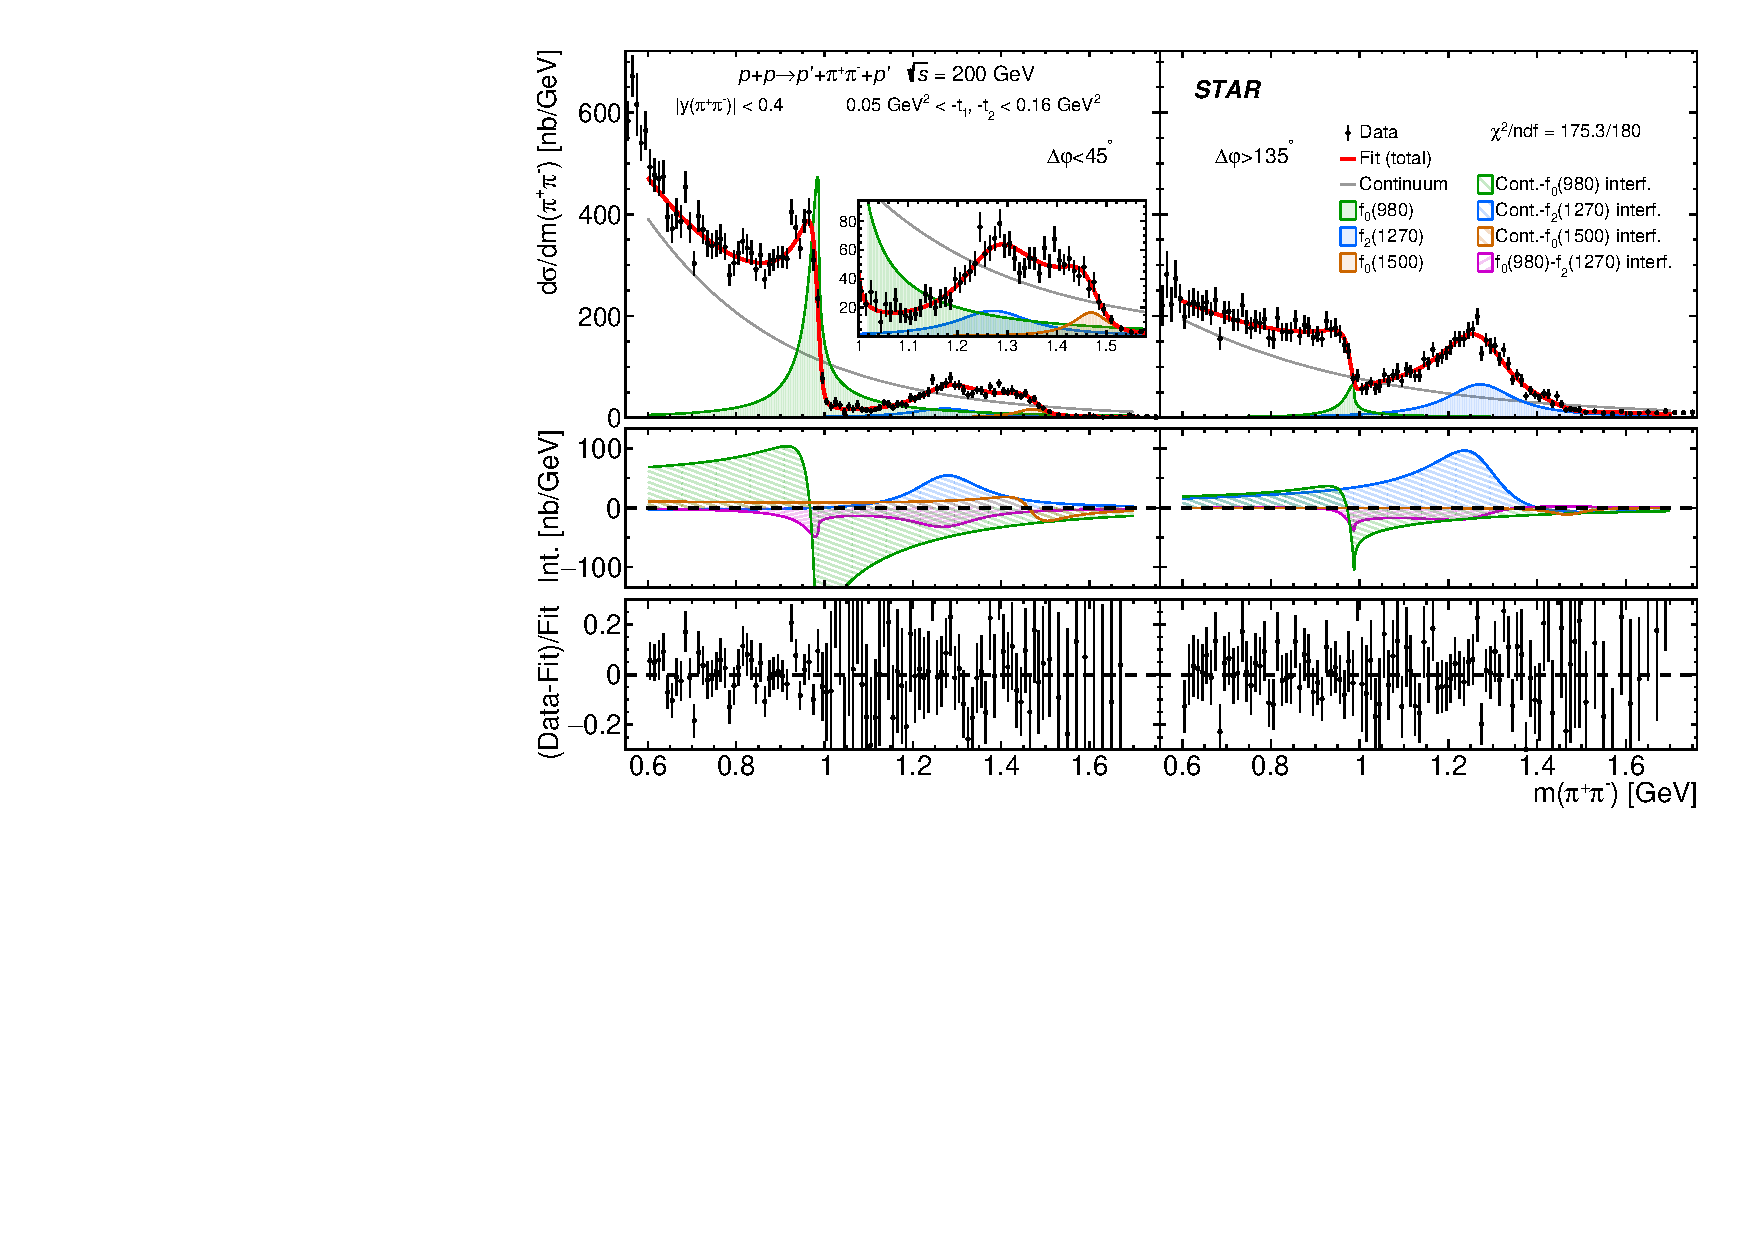
\includegraphics[width=\textwidth,page=1]{graphics/physicsResults/InvMassFit/RatioAndInterference_PiPiInvMass_Fit.pdf}
%
\caption[Differential cross-section $d\sigma/dm(\pi^{+}\pi^{-})$ extrapolated from the fiducial region to the Lorentz invariant phase space given by the central state rapidity $|y(\pi^{+}\pi^{-})|<0.4$ and squared four-momentum transferred in forward proton vertices $0.05~\text{GeV}^{2} < -t_{1}, -t_{2} < 0.16~\text{GeV}^{2}$]{Differential cross-section $d\sigma/dm(\pi^{+}\pi^{-})$ extrapolated from the fiducial region to the Lorentz invariant phase space given by the central state rapidity $|y(\pi^{+}\pi^{-})|<0.4$ and squared four-momentum transferred in forward proton vertices $0.05~\text{GeV}^{2} < -t_{1}, -t_{2} < 0.16~\text{GeV}^{2}$. Left and right parts of the figure show cross-sections for $\Delta\varphi<45^\circ$ and $\Delta\varphi>135^\circ$, respectively. The data are shown as black points with error bars representing statistical uncertainties. Result of the fit $\mathcal{F}(m)$ is drawn with solid black line. The squared amplitudes for continuum and resonance production are drawn with lines of different colors, as explained in the legend. The most significant interference terms are plotted in the middle panels, while the relative difference between each data point and fitted model is drawn in the bottom panel.}
\label{invMassFit}
\end{figure}

The extrapolated cross-sections are shown in Fig.~\ref{invMassFit} together with the result of the fit described above. The model parameters providing minimum $\chi^{2}$ are listed in Tab.~\ref{tab:fitRes}. The fit with the total of 20 free parameters gives $\chi^2$/ndf = 289/200 which shows that the data and model are in reasonable agreement in the fit region. Three resonances are required in the mass range of $0.6-1.7$~GeV: $f_0(980)$, $f_2(1270)$ and $f_0(1500)$. The deviation of the fitted model from the extrapolated data is the most significant at the end part of the fitted mass range, above $1.5-1.55$~GeV. This might result from the presence of $f_{0}(1710)$ and other wide resonances above the fit limits, which are not included in the model.

{
\renewcommand{\arraystretch}{1.5}
\begin{table}[]\centering
\begin{tabular}{ccc c c} ~ & ~ & ~ &\multicolumn{2}{c}{$\bm{ p \pm \delta_{\text{\bf{stat}}} \pm \delta_{\text{\bf{syst}}} \pm \delta_{\text{\bf{model}}}}$} \\ ~ & \bf{parameter} & \bf{unit} & $\bm{\Delta\varphi<45^{\circ}}$ & $\bm{\Delta\varphi>135^{\circ}}$ \\ \hline\hline \multirow{2}{*}{\bf{Continuum}} & $\bm{A}$ & $\bm{\left(\text{\bf{nb/GeV}}\right)^{\frac{1}{2}}}$ & $63.9 \pm 3.8 ^{+4.5}_{-8.1}$ & $35.8 \pm 1.8 ^{+3.0}_{-2.9}$ \\ %\hline
& $\bm{B}$ & $\bm{\text{\bf{GeV}}^{-1}}$ & $6.3 \pm 0.4 ^{+0.1}_{-0.2}$ & $4.7 \pm 0.3 ^{+0.2}_{-0.2}$ \\ \hline
\multirow{5}{*}{$\bm{f_{0}(980)}$} & $\bm{|A|}$ & $\bm{\left(\text{\bf{nb/GeV}}\right)^{\frac{1}{2}}}$ & $20.9 \pm 0.5 ^{+1.1}_{-1.4}$ & $7.8 \pm 0.4 ^{+0.4}_{-0.5}$ \\ %\hline
& $\bm{\phi}$ & \bf{rad} & $0.68 \pm 0.07 ^{+0.02}_{-0.03}$ & $0.54 \pm 0.08 ^{+0.01}_{-0.02}$ \\ %\hline
& $\bm{M}$ & \bf{MeV} & \multicolumn{2}{c}{$955.6 \pm 5.6 ^{+0.9}_{-3.3}$} \\ %\hline
& $\bm{\Gamma_{0}}$ & \bf{MeV} & \multicolumn{2}{c}{$161.6 \pm 21.1 ^{+4.4}_{-3.8}$} \\ %\hline
& $\bm{\sigma}$ & \bf{nb} & $38.7 \pm 3.5 ^{+3.9}_{-4.8}$ & $5.4 \pm 0.7 ^{+0.5}_{-0.6}$ \\ \hline
\multirow{3}{*}{$\bm{f_{2}(1270)}$} & $\bm{|A|}$ & $\bm{\left(\text{\bf{nb/GeV}}\right)^{\frac{1}{2}}}$ & $4.0 \pm 0.4 ^{+0.3}_{-0.3}$ & $7.9 \pm 0.3 ^{+0.4}_{-0.5}$ \\ %\hline
& $\bm{\phi}$ & \bf{rad} & $-1.83 \pm 0.10 ^{+0.03}_{-0.01}$ & $-0.86 \pm 0.04 ^{+0.03}_{-0.03}$ \\ %\hline
& $\bm{\sigma}$ & \bf{nb} & $4.4 \pm 0.9 ^{+0.6}_{-0.6}$ & $16.9 \pm 1.3 ^{+1.9}_{-2.1}$ \\ \hline
\multirow{5}{*}{$\bm{f_{0}(1500)}$} & $\bm{|A|}$ & $\bm{\left(\text{\bf{nb/GeV}}\right)^{\frac{1}{2}}}$ & $4.2 \pm 0.3 ^{+0.3}_{-0.3}$ & $0.9 \pm 0.3 ^{+0.1}_{-0.1}$ \\ %\hline
& $\bm{\phi}$ & \bf{rad} & $0.31 \pm 0.11 ^{+0.09}_{-0.06}$ & $1.45 \pm 0.31 ^{+0.05}_{-0.03}$ \\ %\hline
& $\bm{M}$ & \bf{MeV} & \multicolumn{2}{c}{$1471.7 \pm 6.3 ^{+2.1}_{-1.3}$} \\ %\hline
& $\bm{\Gamma_{0}}$ & \bf{MeV} & \multicolumn{2}{c}{$83.8 \pm 11.0 ^{+2.2}_{-3.0}$} \\ %\hline
& $\bm{\sigma}$ & \bf{nb} & $2.3 \pm 0.4 ^{+0.3}_{-0.3}$ & $0.1 \pm 0.1 ^{+0.0}_{-0.0}$ \\ \hline
\end{tabular}
\caption{Results of the fit described in the text in two ranges of azimuthal angle difference $\Delta\varphi$ between forward scattered protons. Statistical and systematic uncertainties are provided for each parameter.}\label{tab:fitRes}\vspace{-5pt} %temporary
\end{table}
}
%
%

Since the masses and widths of $f_0(980)$ and $f_0(1500)$ are free parameters it is possible to confront their fitted values with the PDG data~\cite{pdg}. In the case of $f_0(980)$ the mass and width is found to be respectively $M_{f_0(980)}=956 \pm 6 (\text{stat.}) ^{+1}_{-3} (\text{syst.})$~MeV and $\Gamma_{0,f_0(980)} = 162 \pm 21 (\text{stat.}) \pm 4 (\text{syst.})$~MeV. Such numbers differ from the PDG estimates of mass ($990 \pm 20$~MeV) and width (from 10~MeV to 100~MeV), nonetheless PDG emphasizes strong dependence of the resonance parameters on the model of amplitude. Some measurements listed in Ref.~\cite{pdg} are in very good agreement with obtained numbers. In addition to this, mass and width of $f_0(980)$ resulting from the fit with the Breit-Wigner form of amplitude gives result $M_{f_0(980)}=972 \pm 1 (\text{stat.}) \pm 1 (\text{syst.})$~MeV and $\Gamma_{0,f_0(980)} = 65 \pm 3 (\text{stat.}) \pm 1 (\text{syst.})$~MeV, albeit with notably worse $\chi^{2}$/ndf of 361/200. These values are in excellent agreement with PDG estimates and $f_0(980)$ parameters from other measurements assuming Breit-Wigner resonance shape~\cite{pdg}. From this we conclude that the structures in the mass spectrum around 1~GeV are indisputably due to interference of $f_0(980)$ with the remaining states, dominantly with the $\pi^{+}\pi^{-}$ continuum.
%
%

For the $f_0(1500)$ we obtain from the fit $M_{f_0(1500)}=1472 \pm 6 (\text{stat.}) \pm 2 (\text{syst.})$~MeV and $\Gamma_{0,f_0(1500)} = 84 \pm 11 (\text{stat.}) \pm 3 (\text{syst.})$~MeV. These numbers also deviate from the PDG averages: $1505\pm 6$~MeV for the mass and $109\pm 7$~MeV for the width. However, numerous measurements on $f_{0}(1500)$ referenced in PDG (and not used for averages calculation) report mass below 1500~MeV and width below 100~MeV, which are consistent with our result. Removing $f_0(1500)$ from the fit doubles the $\chi^2$ to value 590, a 300 standard deviations effect. From above we infer that the shape of $d\sigma/dm(\pi^{+}\pi^{-})$ around 1.4-1.6~GeV - the high-mass part of the $f_{2}(1270)$ region, is determined by the presence of $f_0(1500)$ interfering mainly with $\pi^{+}\pi^{-}$ continuum and also with $f_{2}(1270)$.
%

\begin{figure}%[t]
\centering
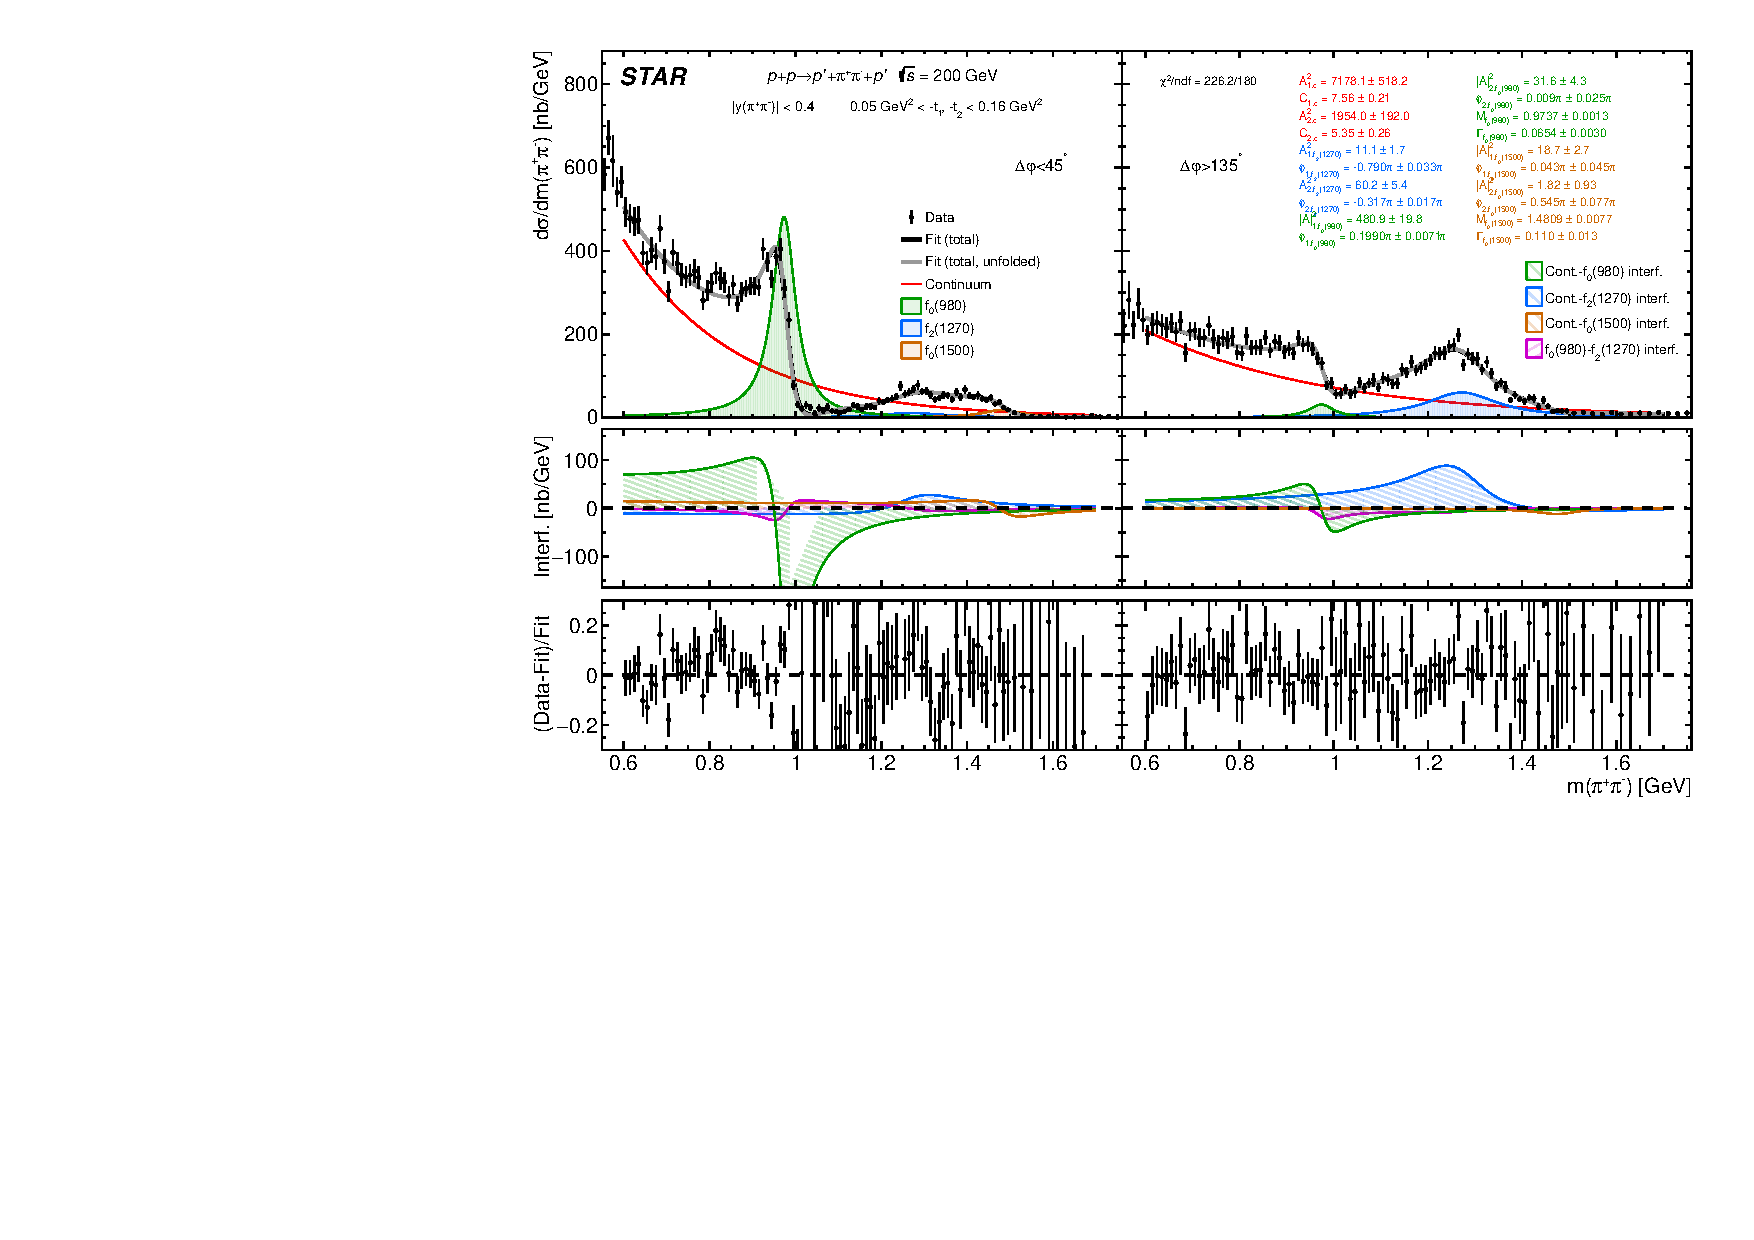
\includegraphics[width=\textwidth,page=1]{graphics/physicsResults/InvMassFit/F0980_BREITWIGNER/RatioAndInterference_PiPiInvMass_Fit.pdf}
%
\caption{Extrapolated $d\sigma/dm(\pi^{+}\pi^{-})$ with the fit assuming Breit-Wigner amplitude for $f_{0}(980)$.}
\label{invMassFit_F0980_BREITWIGNER}
\end{figure}

\begin{figure}%[t]
\centering
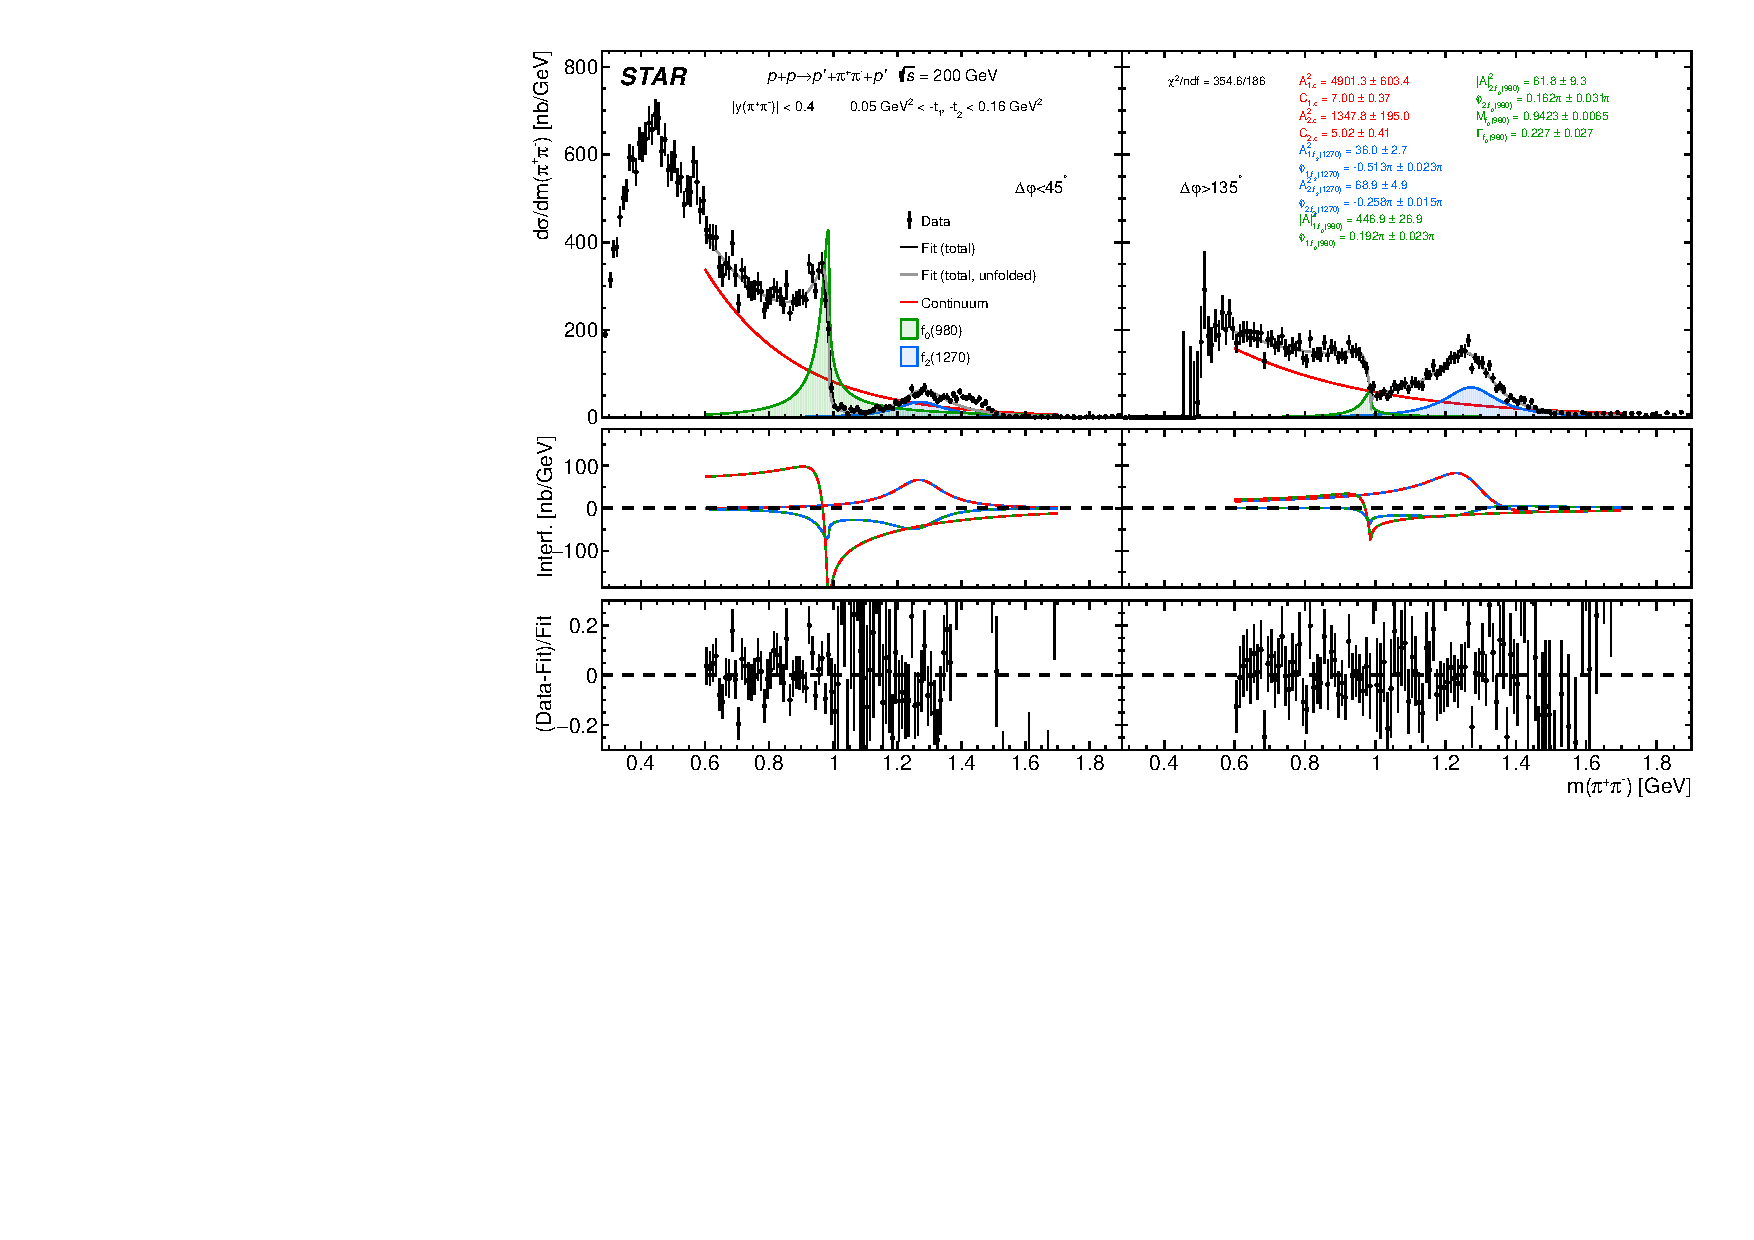
\includegraphics[width=\textwidth,page=1]{graphics/physicsResults/InvMassFit/NO_F01500/RatioAndInterference_PiPiInvMass_Fit.pdf}
%
\caption{Extrapolated $d\sigma/dm(\pi^{+}\pi^{-})$ with the fit ignoring $f_{0}(1500)$ component.}
\label{invMassFit_NO_F01500}
\end{figure}

\begin{figure}%[t]
\centering
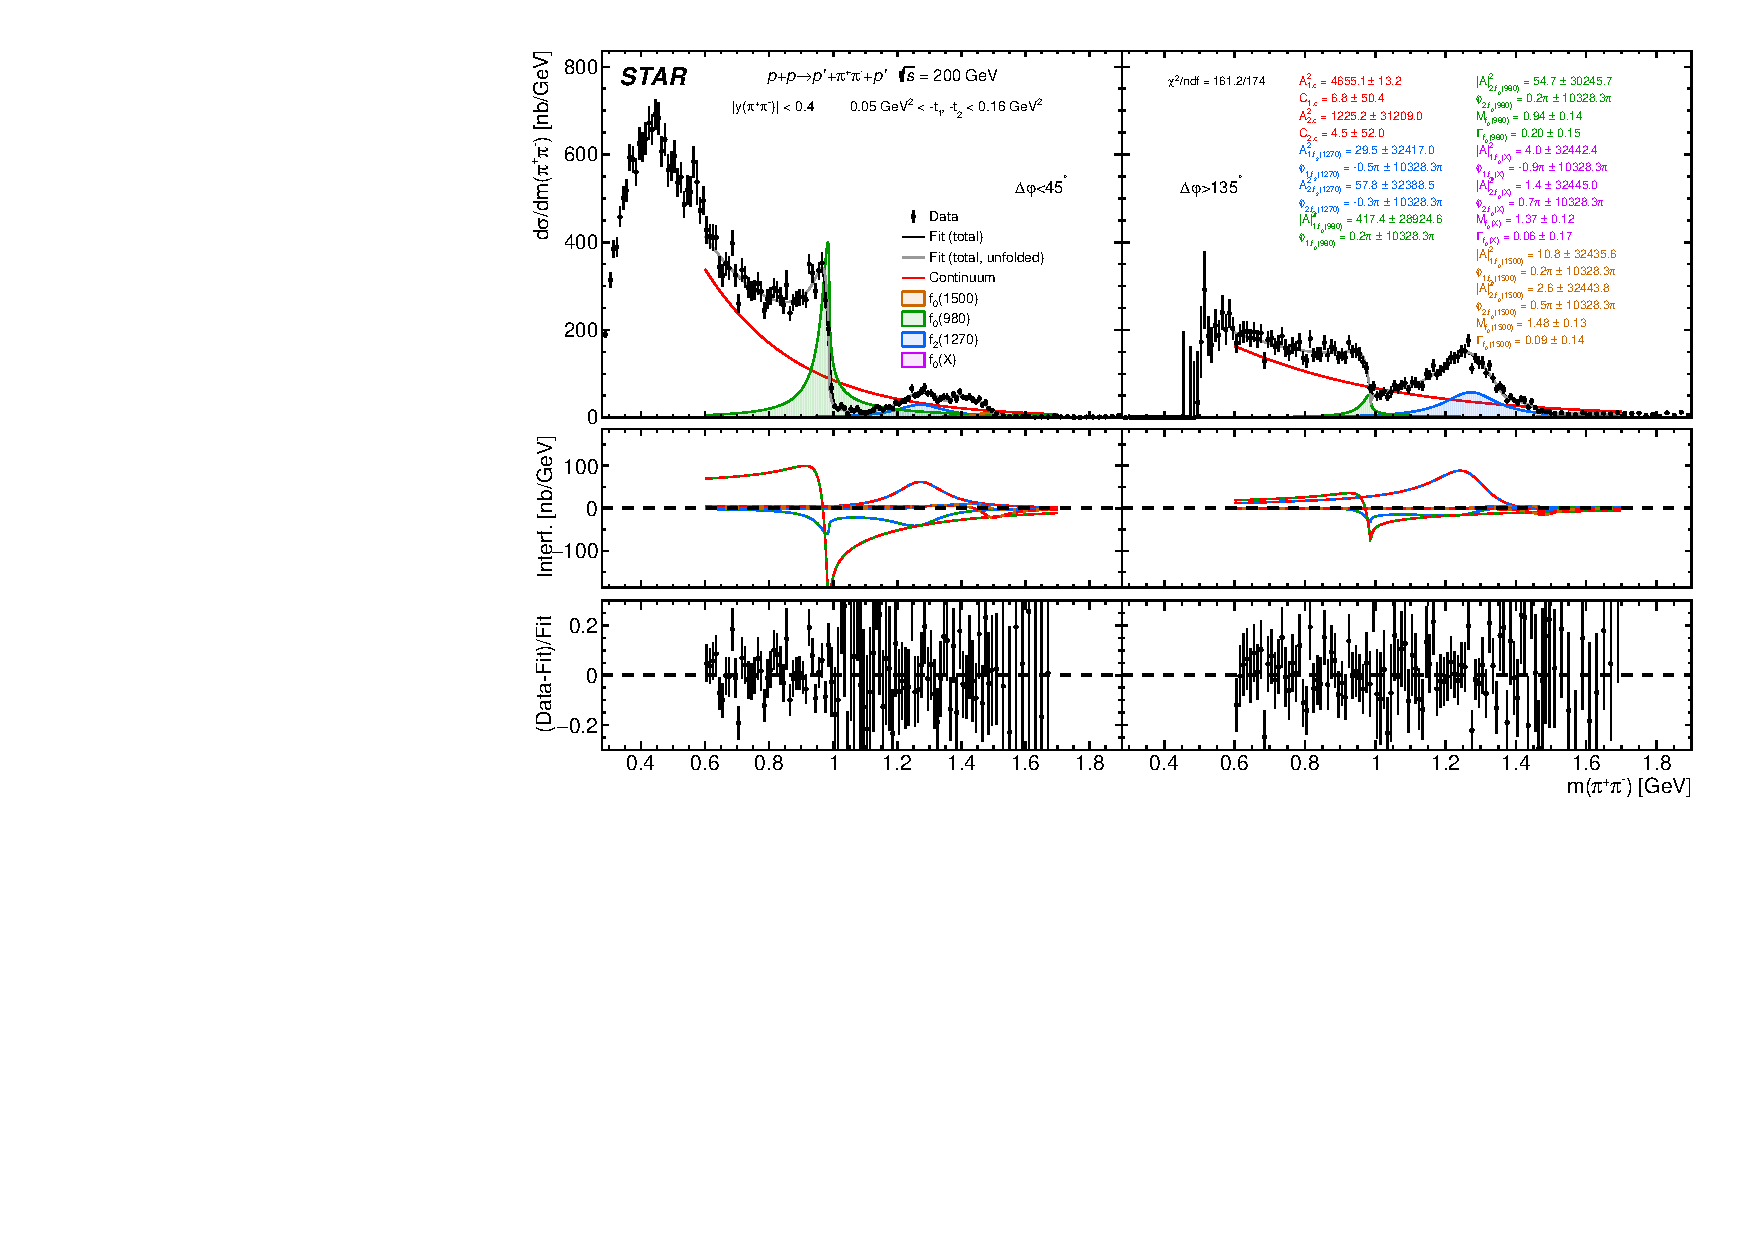
\includegraphics[width=\textwidth,page=1]{graphics/physicsResults/InvMassFit/EXTRA_RESONANCE/RatioAndInterference_PiPiInvMass_Fit.pdf}
%
\caption{Extrapolated $d\sigma/dm(\pi^{+}\pi^{-})$ with the fit accounting for an additional $f_{0}(X)$ component.}
\label{invMassFit_EXTRA_RESONANCE}
\end{figure}


\begin{figure}%[t]
\centering
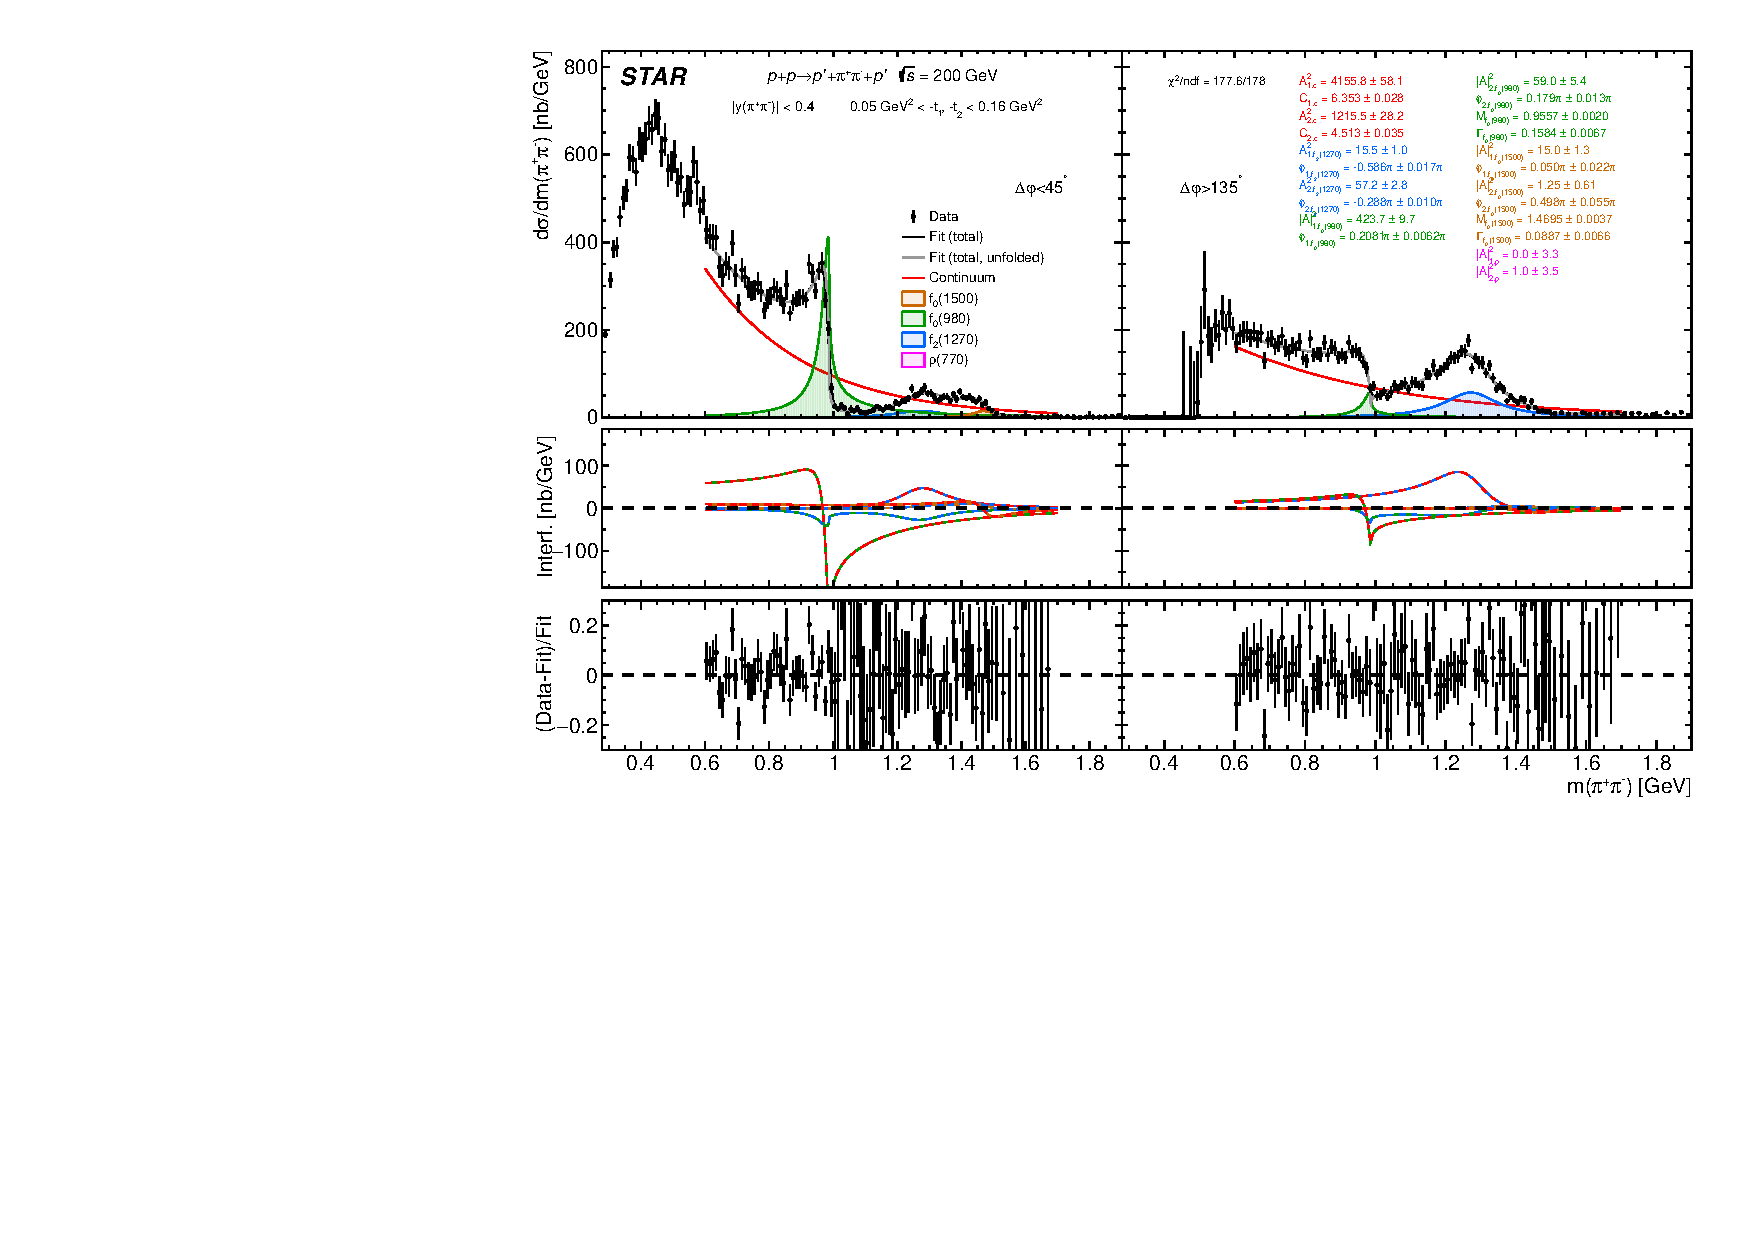
\includegraphics[width=\textwidth,page=1]{graphics/physicsResults/InvMassFit/WITH_RHO/RatioAndInterference_PiPiInvMass_Fit.pdf}
%
\caption{Extrapolated $d\sigma/dm(\pi^{+}\pi^{-})$ with the fit accounting for $\rho_{0}(770)$ production.}
\label{invMassFit_WITH_RHO}
\end{figure}

%

We have tested possibility of existence of an additional resonance produced in CEP between 1.2 and 1.5 GeV. With component $A_{f_0} \times \mathcal{R}_{\textrm{BW}}\left(m;M_{f_0},\Gamma_{f_0}\right)$ added to the model from Eq.~\eqref{eq:amplitude} the best fit is achieved for $M_{f_0}=1326 \pm 9 (\text{stat.})$~MeV and $\Gamma_{0,f_0} = 22 \pm 11 (\text{stat.})$~MeV. In that case the $\chi^{2}$/ndf is improved and equals 270/194 - the dip in $d\sigma/dm(\pi^{+}\pi^{-})$ at $\Delta\varphi<45^{\circ}$ is much better described compared to the nominal fit. Other parameters in the fit change slightly and remain compatible with their original values. Noteworthy is widening of $f_{0}(1500)$ to $\Gamma_{0,f_0(1500)} = 98 \pm 15 (\text{stat.})$~MeV, which gets consistent with the PDG average. The fitted content of additional resonance $f_0$ at $\Delta\varphi<45^{\circ}$ is several times lower than extracted yield of $f_{0}(1500)$, while for $\Delta\varphi>135^{\circ}$ it is consistent with 0. The value of mass agrees with that of $f_{0}(1370)$ resonance, however the obtained width is much lower than PDG estimates of about 200-500~MeV. Given that there are no known resonances of the observed properties we abstain from making definite statements about existence of an additional resonance in the measured exclusive $\pi^{+}\pi^{-}$.
%

From fitted parameters of resonances it is finally possible to calculate integrated cross-section $\sigma$ on their production and decay in the $\pi^{+}\pi^{-}$ channel within earlier defined $|y|$ and $-t$ limits. It is obtained by integrating squared total amplitude on resonance production over entire invariant mass domain. Calculated values of $\sigma$ are provided for each resonance in Tab~\ref{tab:fitRes}. We observe significant dependence of the resonance production cross-section on the azimuthal separation of the forward scattered protons. Two scalar mesons $f_{0}(980)$ and $f_{0}(1500)$ are dominantly produced at $\Delta\varphi<45^{\circ}$, whereas tensor meson $f_{2}(1270)$ - at $\Delta\varphi>135^{\circ}$. This $\Delta\varphi$ dependence is consistent with the observation made by WA102 Collaboration~\cite{WA102}.




% \[A_{\textrm{S-wave}}(m)~~~=~~~A_{\textrm{cont}}\times\sqrt{f_{\textrm{cont}}(m)}~~+~~~~~~~~~~~~~~~~~~~~~~~~~~~~~~~~~~\]\vspace{-15pt}
% \[~~~~~+~~A_{\textrm{f}_0(980)}\times \textrm{BW}\left(m;M_{f_0(980)},\Gamma_{f_0(980)}\right)\]
% \[~~~~~~~~+~~A_{\textrm{f}_0(1500)}\times \textrm{BW}\left(m;M_{f_0(1500)},\Gamma_{f_0(1500)}\right)\]\vspace{-10pt}
% \[A_{\textrm{D-wave}}(m)~~~=~~~A_{\textrm{f}_2(1270)}\times \textrm{BW}\left(m;M_{f_2(1270)},\Gamma_{f_2(1270)}\right)~~~~~~~~~~~~\]\vspace*{-5pt}
% where\vspace{5pt}
% \[A_{\textrm{cont}},A_{\textrm{f}_2(1270)}\in\mathbb{R},~~~A_{\textrm{f}_0(980)},A_{\textrm{f}_0(1500)}\in\mathbb{C}~~~~\rightarrow~~~~A=|A|e^{i\phi}.\]
% 
% Continuum model:
%  \[f_{\textrm{cont}}(m) = (m-2m_{\pi})^{B}\times e^{-C\cdot m}\]
%  Breit-Wigner form (relativistic Breit-Wigner with mass-dependent width):\vspace{-5pt}
% \[\hspace*{-5pt}\textrm{BW}(m;M,\Gamma_{0}) = \frac{M\sqrt{\Gamma_{0}}\sqrt{\Gamma(m)}}{M^{2}-m^{2}-i M\Gamma(m)},~~\Gamma(m) = \Gamma_{0}\frac{q}{m}\frac{M}{q_{0}}\left(\frac{B_{J}((qR)^{2})}{B_{J}((q_{0}R)^{2})}\right)^{2},\]\vspace*{-7pt}
% \[q(m) = \frac{1}{2}\sqrt{m^{2}-4m_{\pi}^{2}},~~~~~~q_{0} = q(M),~~~~~~R=1~\textrm{fm}\]\vspace*{-15pt}
% \begin{itemize}
%  \item masses and widths of $f_{2}(1270)$ are well known therefore they were fixed in the fit (used PDG values)
%  \item fit was done simultaneously to $d\sigma/dm$ in $\Delta\phi<45^{\circ}$ and $\Delta\phi>135^{\circ}$ mass bins
%  \item phases and amplitudes were independent is two $\Delta\phi$ bins, while masses and widths were forced to be the same
%  \item no residual background was accounted since we already subtracted it (background determined using data-driven method, using missing $p_{T}$)
%  \item data were corrected using assumption of the $\pi\pi$ pair being S-wave
% \end{itemize}

